%\documentclass[12pt,ascmac]{jreport}
\documentclass[12pt]{jreport}
\usepackage{sty/eclepsf}
\usepackage{tascmac}
\usepackage{tabularx}
\usepackage[longnamesfirst]{natbib}
\usepackage[dvipdfm]{graphics}
\usepackage[dvipdfm]{graphicx}
\usepackage[dvipdfm]{color}
\usepackage{subfigure}
%\usepackage[dvipdfm, colorlinks, breaklinks,%
\usepackage[dvipdfm, breaklinks,%
bookmarks=true, bookmarksnumbered=true,%
bookmarkstype=toc, bookmarksopen=true,bookmarksopenlevel=3,%
pdftitle={Countermeasure based on risk analysis of collecting digital information },%
%%pdfsubject={},%
pdfauthor={Yuki Uehara},%
pdfkeywords={1.Network Tracking, 2.Digital Forensics, 3. Internet Security, 4.Network Monitoring}%
]{hyperref}

\AtBeginDvi{\special{pdf:tounicode EUC-UCS2}}

\usepackage{fancyhdr}

\usepackage{./sty/doxygenorig}

\usepackage{indentfirst}
\usepackage{url}
\usepackage{listings,sty/jlisting}

\lstset{%
 language={C++},
 %backgroundcolor={\color[gray]{.85}},%
 basicstyle={\small},%
 identifierstyle={\small},%
 commentstyle={\small\itshape},%
 keywordstyle={\small\bfseries},%
 ndkeywordstyle={\small},%
 stringstyle={\small\ttfamily},
 frame={tb},
 breaklines=true,
 columns=[l]{fullflexible},%
 numbers=left,%
 xrightmargin=0zw,%
 xleftmargin=1.5zw,%
 numberstyle={\scriptsize},%
 stepnumber=1,
 numbersep=1zw,%
 lineskip=-0.5ex%
}

\usepackage{amssymb}
%\usepackage{supertabular,multirow}

% A4  size: 297mm*210mm %1pt = 0.35mm
\setlength{\topmargin}{-3.4mm} % 10pt 25.4mm - 3.4mm = 22mm
\setlength{\oddsidemargin}{-0.4mm} % 25.4mm - 0.4mm = 25mm
\setlength{\evensidemargin}{-0.4mm} % 25.4mm - 0.4mm = 25mm
\setlength{\textheight}{231mm} % 660pt % original is 225.75mm 645pt
\setlength{\textwidth}{160mm} % 457pt

\renewcommand{\topfraction}{.99}
\renewcommand{\textfraction}{.0}
\renewcommand{\floatpagefraction}{.99}
\renewcommand{\bibname}{����ʸ��}

\pagestyle{fancy}  
%\rhead{\thepage}
%\rhead[]{\leftmark} 
\lhead[]{} 
%\lhead[\rightmark]{} 

\makeatletter
\def\chaptermark#1{\markboth {\ifnum \c@secnumdepth>\m@ne
\@chapapp\ \thechapter \@chappos\ \fi #1}{}}
\makeatother

\begin{document}


\pagenumbering{roman}

\begin{titlepage}

\begin{center}
\begin{Large}
´����ʸ ~~~~~ 2013ǯ�١�ʿ��25ǯ�١�
\end{Large}
\end{center}

\begin{center}
~ \bigskip ~ \\
\begin{LARGE}
\begin{tabular}{|c|}
\hline
�ޥ������֥�������Ѥ�����ֱ��Ծ�����˥����
\\ \hline
\end{tabular}
\end{LARGE}
\\

~ \bigskip ~ \\
~ \bigskip ~ \\
~ \bigskip ~ \\
~ \bigskip ~ \\


\end{center}
\begin{center}
\begin{Large}
\medskip
���������� �Ķ��������\\
\medskip
��̾��\underline{��ë ů��}\\
\medskip
\medskip
����\\
���������� �Ķ��������\\
¼�� ��\\
���� �ѹ�\\
���� ��Ƿ\\
��¼ ��\\
�⼮ �쵪\\
�Ŷ� �Ϲ�\\
Rodney D. Van Meter III\\
���� ����\\
���� ��\\
��߷ ��\\
���� ����\\
\medskip
{\today}

\medskip
\end{Large}
\end{center}


\end{titlepage}


\thispagestyle{empty}
´����ʸ�׻� - 2009ǯ�� (ʿ��21ǯ��)
~ \\
\begin{center}
\begin{Large}
\begin{tabular}{|c|} \hline
�ǥ������������ˤ��\\
�桼�����פȥꥹ��ʬ�Ϥ��к������
\\ \hline
\end{tabular}
\end{Large}
\end{center}
~  \\
%~ \bigskip ~ \\

%��ʬ�ι׸�����ˡ���¸��γ��פȷ�̡�
%����


%��ʸ���򤳤��Ȥ��Ƥ������ꡢ
���󵻽Ѥ�ȯŸ��ȼ�����ͥåȥ�����ȯ�������ǥ����������ưפ˵�
Ͽ�Ǥ���褦�ˤʤä�������ˤ�äơ����ޤ�ñ�ȤǤϥ桼���θĿ;���Ȥ�
��ʤ��ä������ʣ���Ȥ߹�碌�뤳�Ȥǡ��桼���ץ饤�Х�������������
ǽ�������롥��������˼���Ȥि��ˤϡ��桼�������Ū��ȯ�����Ƥ����
����Ȥ߹�碌���ݤˡ��ɤ����٤ޤǥ桼���ץ饤�Х������������Τ�����
�Τˤ��Ƶ�������ɬ�פ����롥�����ơ��桼���ץ饤�Х����뤿��ˡ�����
�ޤǸĿ;���ȸ����Ƥ��ʤ��ä���Τ�ޤ�ơ�����μ����ȼ�갷���˴�
���륬���ɥ饤������Τ˼����ʤ���Фʤ�ʤ���

����ʸ�Ǥϡ��桼����̵�ռ���ȯ�����Ƥ������μ����ˤ�äơ��桼���ץ�
���Х�������������ǽ�����󼨤��롥�Ŀ;���ˤʤꤦ��桼������ϡ���
������Ԥ��оݤˤʤ�桼���ȤΥͥåȥ���ξ�Ǥδط��ˤ�äƼ����Ǥ�
���ϰϤ��Ѥ�ꡤ�ꥹ�����Ѳ����롥�����ǡ�����Ū�˼�����ǽ�Ǥ���ȸ���
�ޤ������3����󤲡����줾��ξ���ˤ�äơ��桼���Υץ��ե�������
�������ˡ���󼨤���������ʸ�ǥץ��ե�������������Ѥ�������ϡ��ѥ���
�ȤΥإå����󡤥ۥ��Ȼ񸻶�ͭ�˴ؤ������Bluetooth�ǥХ�����õ������
�Ǥ��롥�����3�Ĥξ����¿���Υ桼�������Ū��ȯ�����Ƥ��뤿�ᡤ������
�ưפǤ��롥�����ξ���ˤ�äƤϡ��桼�������ꤹ�뤳�Ȥ��Ǥ���С��桼
���Υͥåȥ���ˤ������ư����䡤�ºݤ�������֤���ʤɡ��桼����
�饤�Х����������������������롥�����ơ��󼨤�����ˡ��¾ڤ��뤿��ˡ�
�ƾ������������Ϥ��륷���ƥ������������ڤ�����̡����Ҥ���3�Ĥξ������
�Ѥ��ƥ桼���Υץ��ե����뤬�����Ǥ��뤳�Ȥ��ǧ������

���������̤˴�Ť���3�Ĥξ�������Ѥ��ƥǡ�����������륱���������ꤷ��
�桼���Υץ饤�Х����Ф���ƶ���ͻ������������ơ��桼���Υץ饤�Х���
�ݸ�뤿��ˡ����ڷ�̤˴�Ť��������ɥ饤�����Ƥ�����


~ \\
�������:\\
\underline{1���ͥåȥ������}, \underline{2. �ե���󥸥å�},
\underline{3. �������ƥ�}, \underline{4���ͥåȥ���ƻ�},
\begin{flushright}
���������� ������������\\
~ \\
\begin{Large}
�帶 ͺ��
\end{Large}
\end{flushright}


\clearpage

\thispagestyle{empty}
Abstract of Bachelor's Thesis - Academic Year 2009
~ \\

%\begin{flushright}
%Academic Year 2008
%\end{flushright}

\begin{center}
\begin{Large}
\begin{tabular}{|c|} \hline
Risk Analysis and Countermeasures on User Tracking \\
by Digital Information Surveillance
\\
\hline
\end{tabular}
\end{Large}
\end{center}
~  \\
\indent As computer networks have covered various places and
population globally, users transmit various data in numerous occasions,
both intentionally and unintentionally.  As services that utilize the
network increased, the chance of data transmitted on the network being
accumulated and recorded has reached the significant level.  Those
individual data may not be considered as privacy information.
However, as those control data has increased, it became possible to
combine them and produce a single profile of a certain user.  When the
profiling become possible, the information that weren't considered as
a privacy information then becomes a privacy information.

To ensure that the users' privacy aren't intruded, it is necessary to
determine which information could lead the profiling of the user, and
construct a guideline based on the study.  This thesis clarifies the
types of information that could be accumulated to profile a user, and
how those information could be captured on the computer network.The
method proposed in the thesis classifies collectors into three
categories, and different methods of profiling is stated based on the
characteristics of those categories.  The information used for
capturing a user's profile includes: packet header information,
information used for sharing hosts' computing resources, and device
discovery information for Bluetooth devices.  The threats that could
outcome from the profiling include: revealing users' activity history,
discovering when the users are actively using the network, and
determining actual location of the physical computer that is being a
source of the information.The system for capturing and analyzing those information was developed
to present that they could be a threat against privacy information.  The
result showed that both specifying an individual user and profiling the
user's activities is possible based on the method presented in the
thesis.

Based on the evaluation,we discussed cases of collecting these imformation and impact of users privacy.
Additionally, the guidelines for handling those information is
proposed, to ensure that the users' privacy are protected and secured.


~ \\
Keywords : \\
\underline{1. Network Tracking}, \underline{2.Digital Forensics}, \underline{3.Internet Security}, \underline{4.Network Monitoring}

\begin{flushright}
Keio University, Faculty of Policy Management\\
~ \\
\begin{Large}
Yuki Uehara
\end{Large}
\end{flushright}

\clearpage

\tableofcontents\thispagestyle{empty} %�ܼ�
\clearpage
\listoffigures\thispagestyle{empty} %���ܼ�
\clearpage
\listoftables\thispagestyle{empty} %ɽ�ܼ�
\clearpage
\pagenumbering{arabic}
\chapter{����}
\label{introduction}
�ܾϤǤϡ��طʤǤ���桼�����ռ�������ȯ�����Ƥ�����󤬡��桼���ץ饤
�Х��򶼤�����ǽ�������뤳�Ȥ�Ҥ٤롥�����ơ��������ǥ������̿������
�ץ饤�Х��Τ���������Ƥ���Ȥ�����Ū�����餫�ˤ���ȤȤ�ˡ�����ʸ��
�����򵭤���
\section{�桼����ȯ���������Ȥ�������}
\label{introduction:intro}
%����������
��ǯ�����󵻽Ѥ�ȯŸ�ˤ�äƥ桼���˴ؤ����͡��ʾ��󤬡��ǥ������̿���
�����������졤��Ͽ�Ȥ��ƻĤ���褦�ˤʤä�������ˤ�äơ��桼���˴ؤ�
��������������Ϥ��뤳�Ȥǡ����������ͤ����߽Ф����Ȥ��Ǥ��롥���Τ�
�ᡤ���桼�����׵�˱����������ӥ����󶡤���ǽ�Ȥʤä�����ɽŪ�ʤ��
�Ȥ��Ƥϥ桼���ι��������¾�桼���ι����������Ӥ���쥳���ǡ�����
�󵻽Ѥ����Ѥ��Ƥ���Amazon\cite{amazon:2009}�䡤���ߤΰ��־���ȹ����
�Ȥ߹�碌�뤳�Ȥˤ�äơ��桼���μ��Ϥ�������������륵����
��NAVITIME\cite{navitime}�ʤɤ��󤲤��롥�����������Τ褦�ʾ��󵻽Ѥ�
ȯŸ�ˤ�äơ�����ޤǤϸĿ;���ȸ��ʤ���ʤ��ä����󤬡��桼���Υץ饤
�Х��򶼤����Ȥ�����ǰ�����롥

%�ץ饤�Х��ˤĤ���
�Ŀ;�������Ѥ��륤�󥿡��ͥåȥ����ӥ��䥳��ƥ�Ĥ����ä���ˤ����ꡤ
�桼���Υץ饤�Х����ݸ��ɬ���������롥���Τ��ᡤ������ͭ�Ԥϸ�̩��
������������褦�ˤʤä����Ŀ;���򰷤�¦�ϡ��Ŀ;���˴ؤ��뵬��
�򵭺ܤ����Ʊ�������ѥץ饤�Х����ݸ���͡��ʵ��Ѥ���Ƥ��Ƥ��롥��
��ʸ�ǽҤ٤�Ŀ;���Ȥϡ��Ŀ;����ݸ�ˡ���������������Ƥ��롤"��
¸����Ŀͤ˴ؤ������Ǥ��äơ���������˴ޤޤ���̾����ǯ��������¾
�ε������ˤ������θĿͤ��̤��뤳�Ȥ��Ǥ����Ρ�¾�ξ�����ưפ˾�
�礹�뤳�Ȥ��Ǥ�������ˤ������θĿͤ��̤��뤳�Ȥ��Ǥ��뤳�ȤȤʤ�
��Τ�ޤ��"\cite{privacy_policy:2009}��ؤ��������ơ��ץ饤�Х���
��Privacy and Freedom\cite{privacy:1967}�ǽҤ٤Ƥ��롤"�軰�Ԥ��������
�ؤ���Ŀ;����ɤ����ټ������뤤�϶�ͭ���뤳�Ȥ��Ǥ��뤫����������
���븢��"��������롥

�桼���Υץ饤�Х�����ǰ�������������󤲤롥�ǥ�����ǥХ��������ä�
��äơ��桼���ϰտޤ�����¿���ξ����ȯ�����Ƥ����礬���롥���κݤˡ�
���Ȥ˴ؤ����󤬴ޤޤ�Ƥ�����䡤���οͤȴؤ�꤬��������ȯ����
�Ƥ����礬���롥�ޤ����ͥåȥ����Ǥξ����ʣ�����Ȥ߹�碌�뤳��
�ǡ�������Τ˸ĿͤΥץ��ե������������뤳�Ȥ��Ǥ��롥����ˤ�äơ�
ʣ���ξ�����Ȥ߹�碌�뤳�Ȥˤ�äƥͥåȥ���ˤ�����桼����Ĵ���䡤
Ĵ���ˤ�ä�����줿���׾����������뤳�Ȥˤ�뿷���������ӥ��䡤�Ⱥ�
�ܺ��ʤɤ����ѤǤ���ȿ�̡��桼���Υץ饤�Х�����������ĤĤ��롥

%�ץ饤�Х��ˤĤ��Ƥ�������
���ߡ��桼���Υץ饤�Х����ݸ��¿���ε��Ѥ���Ƥ���Ƥ��뤬���ǥ���
��ǥХ��������äˤ�äơ��桼�������Ȥξ�����Τ餺�˸������Ƥ�����
�䡤���ޤǤϸĿ;���Ȥʤ�ʤ��ä���������礹�뤳�Ȥˤ�äơ��桼��
���ȤΥץ饤�Х�������������ǽ�������롥����ϡ��ɤΤ褦�ʾ��󤬼��Ȥ�
�ץ饤�Х��򶼤�����Ƥ��뤫�Τɤ����٤θ��¤���ĥ桼���ޤ��Τ뤳�Ȥ�
�Ǥ��뤫�Ȥ�������ʬ����ۣ�������Ǥ��롥����������褹��ˤϡ�
�ɤΤ褦�ʾ���ˤ�äƥ桼���Υץ饤�Х������������Τ����Τˤ��ơ��桼
�����Ȥ⤽����Τ�ɬ�פ����롥

%�Ǥ⥳��ƥ�ĶȼԤϻȤ�������͡�
����������ƥ�Ĥ䥵���ӥ��󶡼ԤϸĿ;�������ΨŪ�˼�������ɬ�פ�����ȿ�̡�
Ʊ���˥桼���Υץ饤�Х����ݸ���θ������ʤ���Фʤ�ʤ�������
���뤳�Ȥ��Ǥ�����󤹤٤Ƥ����Ѥ�����硤�桼���Υץ饤�Х��ζ��ҤˤĤʤ�
���ǽ�������롥���Τ��ᡤ����ƥ�ġ������ӥ��󶡼Ԥϼ�������桼����
������������뤫���⤷�������¤򤷤���Ǿ�����������ɬ�פ����롥


%�����ǽ��֤Ǥ���
\section{�ܸ������Ū}
\label{introduction:purpose}
����ʸ����Ū�ϡ��ǥ�����������ˤ����뿷�����ץ饤�Х��Τ���������
���뤳�ȤǤ��롥�ɤΤ褦�ʾ��󤬥桼���Υץ饤�Х��򿯳����뤫�����Τ�
�����ȤȤ�ˡ�����μ�갷���ˤĤ��Ƹ�Ƥ���롥¿���Υǥ����뵡�������
Ū�����Ѥ���褦�ˤʤä����Ȥǡ��桼���⥵���ӥ��󶡼Ԥ�ɤΤ褦�ʾ���
��ȯ������Ƥ��ꡤ�ɤΤ褦�ʱƶ���⤿�餹���İ�������Ƥ��ʤ��������ǡ�
����ʸ��ä�����줿�θ����󼨤��뤳�Ȥˤ�äơ�ISP��Ϥ���Ȥ���ͥå�
��������Ԥ䡤�����ӥ��󶡼ԡ����ץꥱ�������ȯ�Ԥϡ��ɤΤ褦�ʾ�
�󤬥桼���Υץ饤�Х��򶼤��������İ������Ŀ;�������ΤʻؿˤΤ�Ȥ�
�ݸ�뤳�Ȥ��Ǥ��롥�ޤ����桼�����Ȥ⡤�ɤ�ʾ������ʤ���Фʤ�
�ʤ������Τ뤳�Ȥǡ����ȤΥץ饤�Х�����ʤ���Фʤ�ʤ����ץ饤�Х�
���ݸ�ȡ��������ϥȥ졼�ɥ��դǤ��ꡤ�ɤ��ޤǵ��Ƥ����Τ����Τʶ�ʬ
����ɬ�פǤ��롥�桼���Υץ饤�Х����ưפ˿�������ʤ��Ҳ��¸����뤿��
�ˤϡ��ͥåȥ�������ԡ������ӥ��󶡼Ԥȥ桼��¦����������Ŀ;����
�ؤ����ݸ�򤷤ʤ���Фʤ�ʤ����äˡ��桼�������Ȥ˴ؤ������������
�뤳�Ȥ����桼���Υץ饤�Х����Ф��붼�Ҥ��㸺�Ǥ����ǽ�����⤤���桼
�������Ѥ�������������뤳�Ȥˤ�äơ�����μ�����򤬤Ǥ��뤫��Ǥ�
�롥������������ϥ桼�����ɤξ����ȯ�����Ƥ褤���ΤäƤ��뤳�Ȥ�����
�Ǥ��롥

����ʸ�Ǥϥ桼����̵�ռ���ȯ�����Ƥ������ˤ�äơ��桼���Υ�
�饤�Х����ɤ����ٶ�������Ƥ��뤫��Ĵ�����¾ڤ��롥���μ���Ȥߤˤ��
�ơ��桼�����Ȥ��ɤΤ褦�ʾ����¾�Υ桼���˼��������ȥץ饤�Х���
��������ǽ�������뤫��ޤȤ��ȤȤ�ˡ��ɤξ��󤬤ɤ�Ω��Υ桼����
���Τ뤳�Ȥ��Ǥ��뤫�Ȥ�����ʬ�������Τˤ��롥�㤨�С��桼���ι�ư����
�ϥͥåȥ�������Ԥ����Ǥʤ�Ʊ���ͥåȥ������³���Ƥ���桼���ޤ�
�Τ����뤫�Ȥ���Ĵ���ʤɤ��󤲤��롥


%�����ơ����󥿡��ͥåȤ�ޤ�ǥ������̿��ˤ�����桼���Υץ饤�Х��θ���
%�򼨤���Ʊ���ˡ��ǥ�����������������ǡ��桼���Υץ饤�Х��򶼤���
%�������������Ѥ����ˡ���󼨤������ڤ��롥

����ʸ�Ǥ�����Ū�˥桼����ȯ�������������Ѥ��뤳�Ȥǡ��ץ饤�Х�����
��������ǽ���Τ����ˡ��3�ļ��������Ф��Ƹ��ڡ��ͻ����롥����ˤ�äơ�
�ɤ��ޤǸĿ;����������뤳�Ȥ��Ǥ���Τ������Τ��롥�ܸ���ϥѥ��å�
�Υإå����󡤶�ͭ�ۥ���̾��Bluetooth�ǥХ���̾���Ѥ������ˡ��Ŀ;���
����������ˡ���󼨤������ڤ��롥�����ξ���ϡ��桼��������ȯ���Ƥ�
�����Ǥ��뤿�ᡤ�ưפ˼�����ǽ�Ǥ��롥���Τ��ᡤ�����ξ��󤬥桼��
�Υץ饤�Х��򶼤����Ƥ��뤫�Τ����ɬ�פ����롥

�����θ��ڷ�̤�Ƨ�ޤ��ơ��Ŀ;������ѻ��ˤ�����ץ饤�Х����ݸ����
Ū�Ȥ��������ɥ饤�����Ƥ��롥����ˤ�ꡤ�桼�����Ȥ�ͥåȥ����
���ԡ����ץꥱ�������ȯ�Ԥʤɤ�Ω���̤ˡ��ץ饤�Х���뤿��ˤϡ���
�ξ�����ꡤ�ޤ���ȯ�����Ƥ����꤬�ʤ����Ȥ��������������Τˤ��뤳��
����Ū�Ȥ��롥

\section{����ʸ�ι���}
\label{introduction:organization}
\indent ����ʸ����\ref{conclusion}�Ϥ��鹽������롥
��\ref{background}�ϤǤϡ��ǥ��������μ�����ˡ�ȥ桼���Υץ饤�Х���
���ҤȤʤ����ˤĤ��ƽҤ٤롥��\ref{related_works}�ϤǤϡ�
��\ref{background}�ϤǽҤ٤�����˼���Ȥ��Ϣ�����Ҳ𤹤롥
��\ref{assumption}�ϤǤϡ��ɤΤ褦�ʾ�����Ȥ߹�碌��ȥ桼���ζ��Ҥ�
�ʤ뤫��Ĵ���������μ�ˡ����Ƥ��롥��\ref{evaluation}�ϤǤϡ�
��\ref{assumption}�ϤǽҤ٤���ˡ��Ƥ�������μ¸���̤ˤĤ��ƽҤ٤��
�Ȥ�ˡ��ͻ���Ԥ�����\ref{consideration}�ϤǤϡ���\ref{evaluation}�Ϥ�
���ڤ�����ˡ���к��Ȥ��ơ������ɥ饤�����Ƥ��롥�Ǹ��
��\ref{conclusion}�Ϥ�����ʸ�η����ȡ������Ÿ˾��Ҥ٤롥


%%% Local Variables:
%%% mode: japanese-latex
%%% TeX-master: "../nakajima_bthesis"
%%% End:

\chapter{�ط�}
\label{background}
�ܾϤǤϡ��ż֤��ٱ�˴ؤ���͡��ؤαƶ���Ŵƻ��Ҥ��ԤäƤ�������ξ���ȯ����
�Ĥ��ƽҤ١��������������������򼨤������β��Τ��������ʸ����Ƥ���ӥå��ǡ���
���Ϥ˴�Ϣ�������Ѥ並��ˤĤ��ƽҤ٤롥

\section{�ż�}
�ż֤�¿���οͤ��̶С��̳ؤμ��ʤȤ��Ƴ��Ѥ���Ƥ��롥���������ٱ�䱿�Ը�
��碌�ʤ��������⤢�롥����Ǥϡ��ż֤���������Ŵƻ��Ҥ��ԤäƤ��������
�б��ˤĤ��Ƽ�����

\subsection{�ż֤�������}
\label{background:railroads:problems}
\begin{figure}
    \begin{center}
      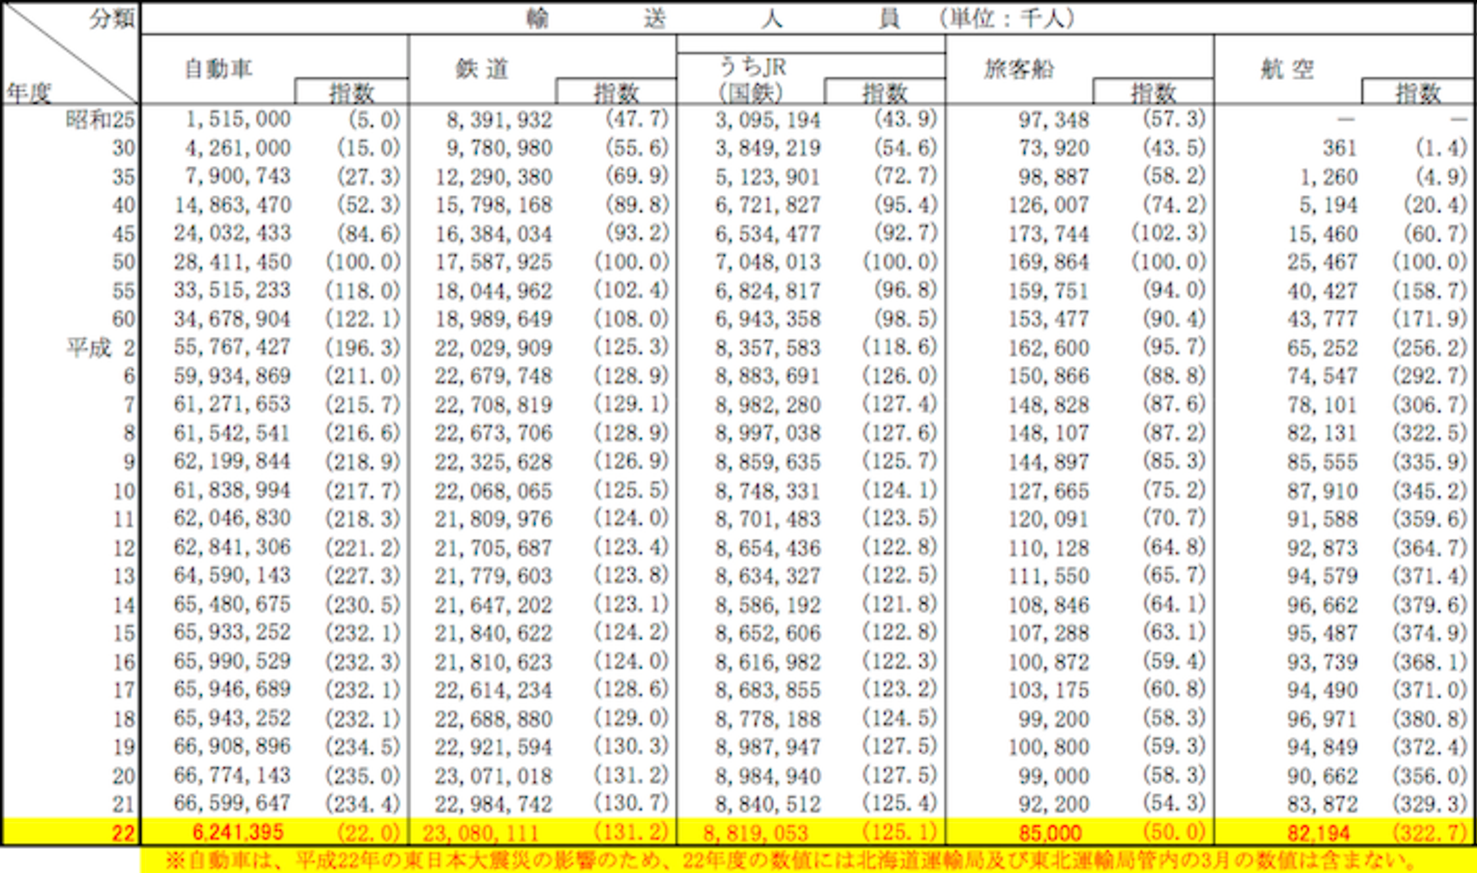
\includegraphics[scale=0.60]{./pdf/kokudokotsusho_users_num}
      \vspace{-5mm}
      \caption{���ܤ�͢��������͢���Ͱ���}
      \label{fig:kokudokotsusho_users_num}
    \end{center}
\end{figure}

���ܤˤ����ơ�¿���οͤ��̶С��̳ؤμ��ʤȤ����ż֤���Ѥ��Ƥ��롥�ż֤�
������û���֤�Ĺ��Υ��ư���뤳�Ȥ��Ǥ���Ȥ������Ǥ��롥�ޤ��֤Ȱ㤤ƻϩ
�ν��ڤ�ʤ�������ɽ�̤�˱��Ԥ��Ԥ��뤿�����ѼԤ����Τʰ�ư���֤��θ
����������Ѥ��뤳�Ȥ��Ǥ��롥���Τ��ᡤ�͡��ʾ��̤��͡��ʿͤ˳��Ѥ����
���롥���ڸ��̾ʤ���ɽ���Ƥ���ι�Ҥ�͢��������͢���̤�
��\ref{fig:kokudokotsusho_users_num}\cite{kokudokotsusho:num_of_users}
�ˤ��ȡ�ǯ����230���ͤ����ܿͤ����̤μ��ʤȤ����ż֤���Ѥ��Ƥ��롥�ż�
�����ѿͿ���¾��͢�����ؤ���¿�������ܤˤ������ż֤ϤȤƤ���פ�����
�̤����Ƥ��롥
\\

���������������⤢�롥���֤����ΤǤ���Ȥ������Ȥ���¿���οͤ˳��Ѥ����
�����ż֤��������Τ����������ʤɤˤ�ä��ٱ�䱿�Ը���碌�ʤɤ������Ƥ�
�ޤ����Ȥ�¿�����롥���ηкѥ���饤��ε���\cite{delay:higaigaku}�����
�������ֶ����ˤ��ȡ��ż֤��ٱ�ˤ���Զ���ؤ��̶Фˤ�����Ҳ�Ū���Ѥ�
ǯ��2180���ߤˤ�ʤ�ȿ�¬����Ƥ��롥���Τʿ����Ȥϸ����ʤ������ż֤���
�ѼԤˤȤä��ż֤��ٱ䤬�ȤƤ�¿����»����Ϳ���Ƥ���ȸ����롥
\\
%http://toyokeizai.net/articles/-/10756

\subsection{Ŵƻ��Ҥ��ٱ���Ф����б�}
\label{background:railroads:correspondence}
\begin{figure}
    \begin{center}
      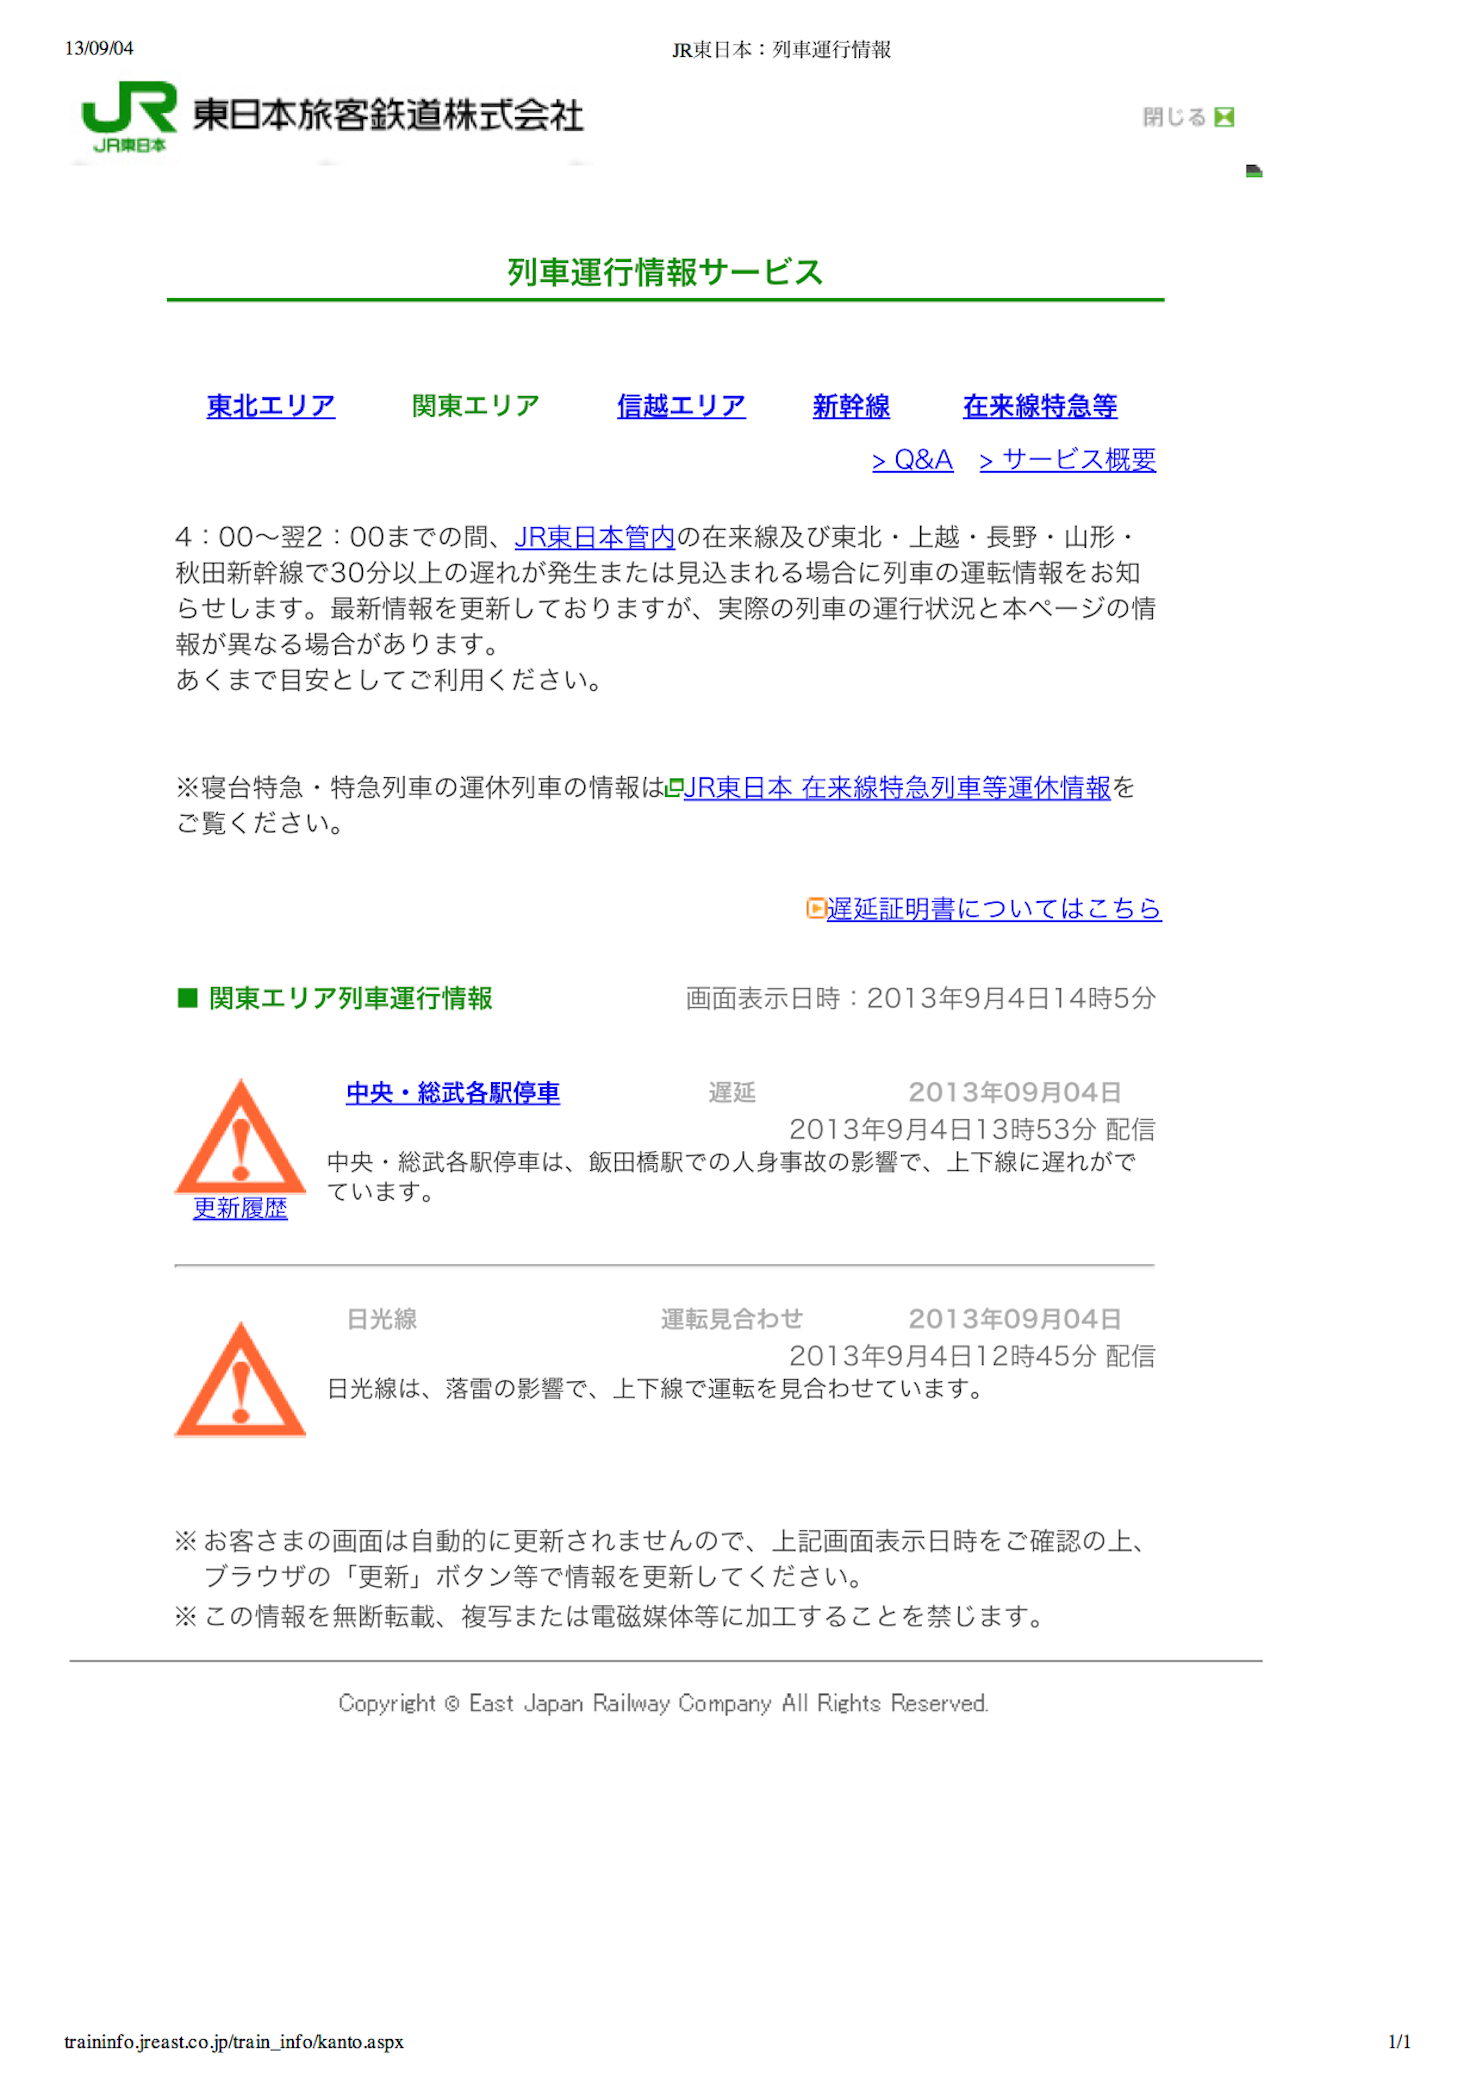
\includegraphics[scale=0.60]{./pdf/jr_delays_page}
      \vspace{-5mm}
      \caption{JR��ֱ��Ծ��󥵡��ӥ��ڡ���}
      \label{fig:jr_delays_page}
    \end{center}
\end{figure}
\begin{figure}
    \begin{center}
      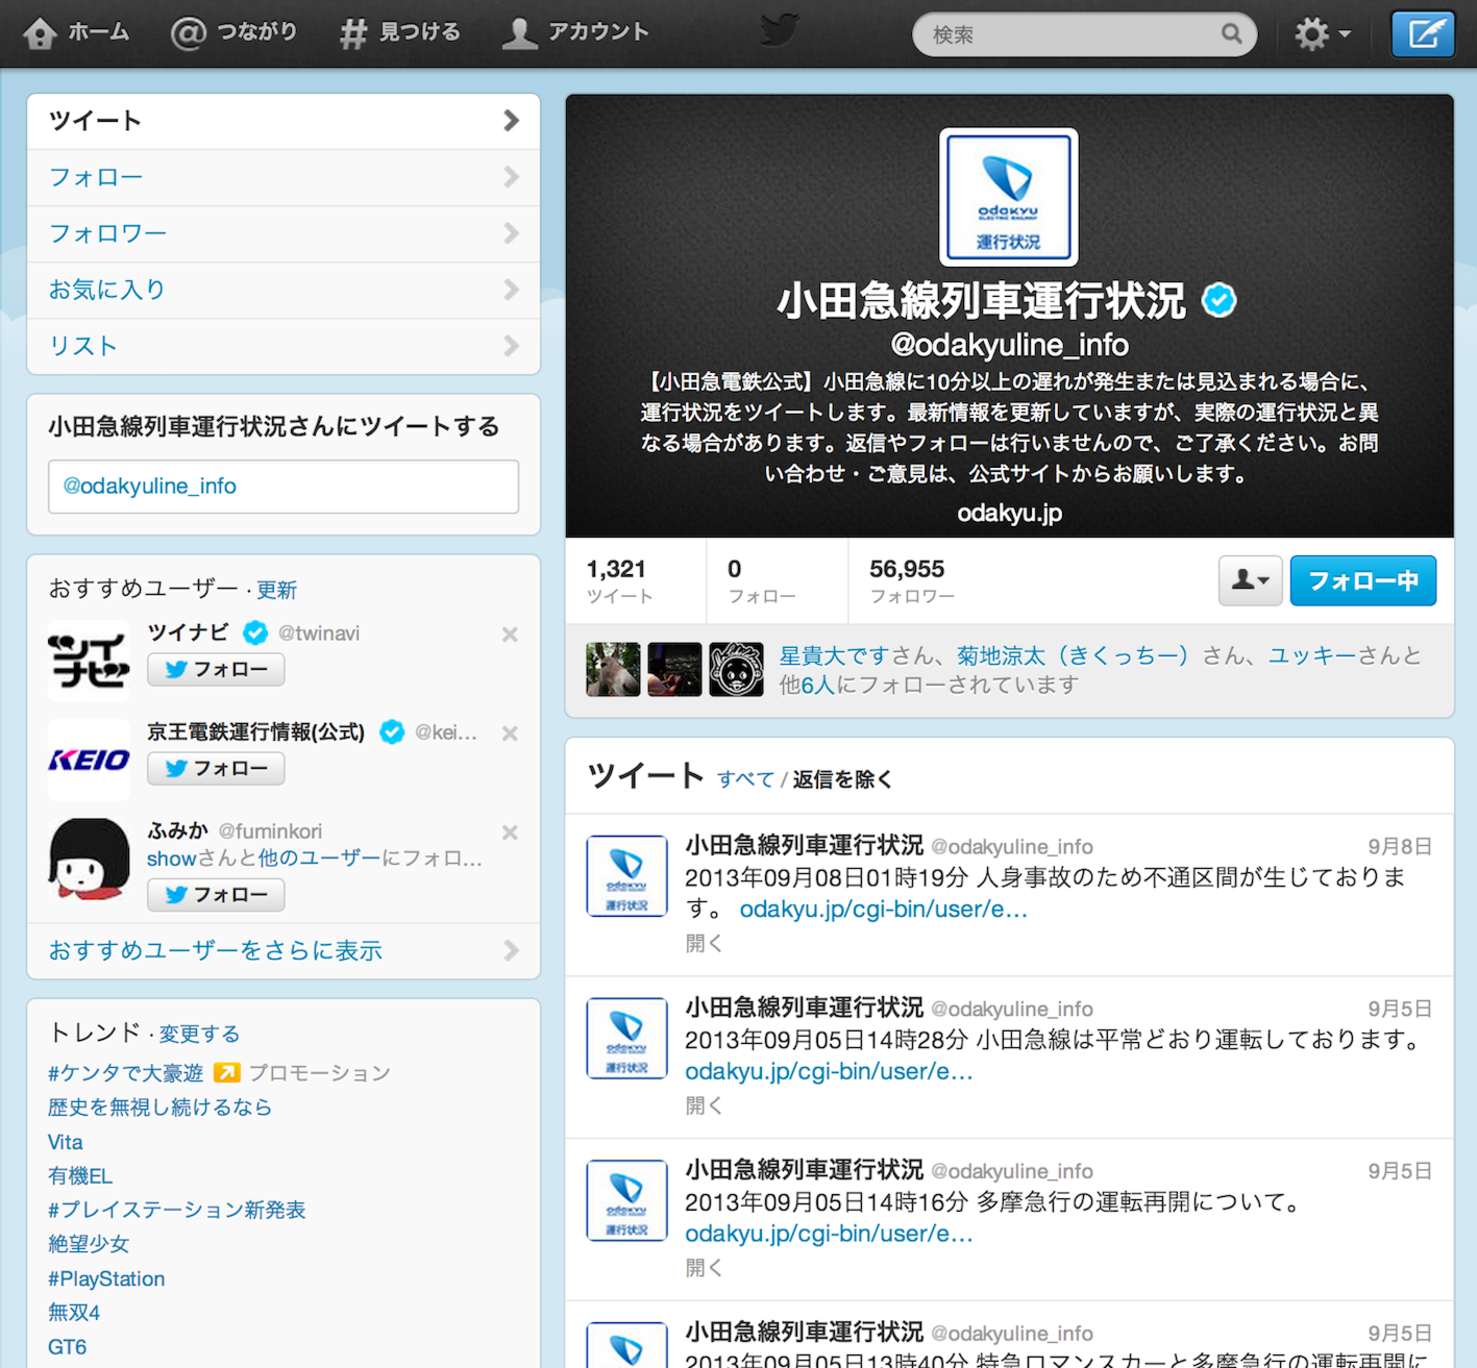
\includegraphics[scale=0.60]{./pdf/odakyu_twitter_page}
      \vspace{-5mm}
      \caption{���ĵ���Twitter��������ȥڡ���}
      \label{fig:odakyu_twitter_page}
    \end{center}
\end{figure}

�ż֤��ٱ�䱿�Ը���碌�ʤɤˤ�äơ�����ɽ�̤�α��Ԥ�Ԥ��Ƥ��ʤ�����
��¿�����롥�ٱ�䱿�Ը���碌���Ф��ơ���Ŵƻ��Ҥ��͡����б���ԤäƤ�
�롥�ꥢ����б��Ȥ��Ƥϡ��Ź��Ǽ��Ĥ˾�����ɽ����ؤ��ٱ����������ۤ�
�ɤ��Ԥ��Ƥ��롥�ꥢ����б��Ϥ��ξ�˹Ԥ��ʤ�����ż֤α��Ծ������Τ�
���Ȥ��Ǥ��ʤ����ᡤ���ѼԤˤȤäƤϤȤƤ��Թ礬���������Τ��ᡤ�ؤ˹Ԥ�
�����ż֤α��Ծ������ǧ�Ǥ���褦�˳�Ŵƻ��Ҥϥ���饤��Ǿ����ȯ����
�Ƥ��롥����饤��Ǥξ���ȯ���λ�����ʲ��˵󤲤롥
\begin{description}
\item {(1)} ���������Ȥˤ����ֱ��Ծ����󶡥ڡ���\\
����Ŵƻ��ҤϤ��줾��Web�����Ȥ���äƤ��뤳�Ȥ�¿����������Web������
�Ǥϴ�Ⱦ��󡤥˥塼�����õޥ����åȤ�ͽ��ʤ��͡��ξ���ȯ������Ƥ��롥
�����ξ����1�ĤȤ��ơ���֤α��Ծ�����ȯ�����Ƥ���ڡ�����¸�ߤ��롥
��\ref{fig:jr_delays_page}\cite{jr:service_status}�Τ褦�˱ؤ˹Ԥ�������
�֤α��Ծ�����Τ뤳�Ȥ��Ǥ��롥���Υڡ����򤦤ޤ����Ѥ���С����٤��Ƥ�
��ϩ������򤷥���������Ȥ��ʤɱؤ˹Ԥ����˺����η�ϩ�����򤹤뤳�Ȥ���
���롥���������������⤢�롥��������Ȥ������Ȥ⤢���ٱ�䱿�Ը���碌��
�ɤ�ȯ�����Ƥ����ۿ��ޤǻ��֤�������Ȥ������Ǥ��롥���Τ��ᡤ����ο���
���Ϲ⤤���ꥢ�륿�����˳������
\item {(2)} Twitter�������������\\
��Twitter�˸�����������Ȥ���äƤ���Ŵƻ��Ҥ⤢�롥���Υ�������Ȥ�ե�
�������뤳�Ȥˤ�äơ�Twitter���äƤ���桼����Twitter�򸫤Ƥ�������ż�
�α��Ծ�������뤳�Ȥ��Ǥ��롥\ref{fig:odakyu_twitter_page}\cite{twitter:odakyu}
���������������⤢�롥������������ȤʤΤǾ��������Τ�ΤʤΤǡ�����
�����ƤޤǤ˻��֤�������ޤ����ޤ�����Ƥ�������ϼºݤ�ȯ�����Ƥ�
���ٱ���⾯�ʤ���
\end{description}


\section{SNS}
SNS�Ȥϡ����������ͥåȥ���󥰥����ӥ���Social Networking Service�ˤ�
ά�Ǥ��롥�Ҳ�Ū�ͥåȥ����Web��˹��ۤ��뤳�ȤǤ��뤬�����ӥ��ڤӥ�����
�Ǥ��롥����Ū�ʵ�ǽ�Ȥ��ơ��ץ��ե����뵡ǽ����å�������ǽ���桼���֤ˤ�
������ߥ�󥯵�ǽ�ȸ�����ǽ���֥�����ǽ�����ߥ�˥ƥ���ǽ�ʤɤ����롥���
����ü������ڤˤ�äơ���ڤ����Ѥ��뤳�Ȥ���ǽ�ˤʤ�¿���οͤ˳��Ѥ����
���롥�����Ǥ�Facebook��Twitter��Google+�����ܤǤ�Mobage��GREE��Ameba��mixi
�ʤɤ����ꡤ¿���οͤ����Ѥ���Ƥ��롥

\subsection{��������륻�󥵤Ȥ��Ƥ�SNS}
�������SNS�桼����������SNS���̤����͡��ξ����ȯ�����Ƥ��롥��ʬ�伫ʬ��
����ξ������̿����ɤ���˥塼���ε����ʤɤ���Ƥ��뤳�Ȥˤ�äơ�SNS���
¾�Υ桼���˸����ƾ����Ȼ����Ƥ��롥�ޤ�SNS�ξ���ȯ�����Ȼ����ԡ��ɤϥƥ�
�ӡ��饸������ʹ��������Ҥʤɤ���ٰ���Ū���ᤤ��This just in��News no 
longer breaks, in Tweets�Ϥ���IT���󥵥륿��Ȥ������ޡ��ӥ󡦥�ǥ���
�������줿�ݡ����ΰ����Ͻ���Twitter�˥ꥢ�륿�������Ƥ��Ƥ������Ȥ򵭻�
�ˤ�����ΤǤ��롥����Ǥ���С����Ԥ��ܿͤ˼�ष�����ˤ��ƴ�¸�Υ�ǥ���
���̤��ƥ˥塼���Ȥ����������˸��������Ϥ��Ǥ��ä�����������Twitter����
���ƥꥢ�륿����˾���ȯ�����Ȼ����줿���Ȥˤ�äơ��Х饯�����Х���������
�۵�������ȯɽ�������ޡ��ӥ󡦥�ǥ���򻦳��������Ȥ����餫�ˤ�������¿��
�οͤ����Τ��Ȥ��ΤäƤ��������λ��¤�Twitter�ʤɤ�SNS���ꥢ�륿��������
�⤤����ȯ�����ΤǤ��뤳�Ȥ������������Ǥ��롥��������̺ҤǤ�Twitter��
facebook���οͤ��²�ΰ��ݡ��Ͽ̤��ﳲ�������ż֤α��Ծ����ˤĤ��Ƥξ���
�����μ��ʤȤ��ƤȤƤ���פ�����̤���������ǯ�Ǥϡ��ͤ�ʪ�����󥵤�Ʊ��
�ε�ǽ����İ��Υ��󥵤ȹͤ�������������ǥ�������Ѥ��ƥꥢ�륿�����
���������¬����Ȥ����ͤ������ޤ줭�Ƥ��롥

%http://jp.techcrunch.com/2011/05/02/20110501news-of-osama-bin-ladens-death-spreads-like-wildfire-on-twitter/


\section{�ӥå��ǡ���}
�ӥå��ǡ����Ȥϡ�����Υǡ����١��������ġ����ǡ����������ץꥱ����
���ǤϽ�������Τ�����ʤۤ����̤ʥǡ�������Τ��ȤǤ��롥

\subsection{�ӥå��ǡ�������ħ}
�ӥå��ǡ�������ħ�Ȥ���3V�Ȥ������դ����롥3V�Ȥϡ��ӥå��ǡ���������
��Value�ˡ������Variety�ˡ����١�Velocity�ˤ�3�Ĥ���ħ�Τ��ȤǤ��롥
�ʲ��Ǥ��줾�����ħ�ˤĤ����������롥
\begin{itemize}
\item ���̡�Volume��\\
��ǯ����Х���ü������ڤ�ȼ��¿���οͤ����󥿡��ͥåȤ���Ѥ���褦��
�ʤä������Τ��ᡤ���󥿡��ͥåȤ����Ѥ����ǡ���������ˤʤäƤ��Ƥ�
�롥����������SNS�Ǥ���facebook��2012ǯ8�������500TB�Υǡ���������
���Ƥ��롥Twitter��2011ǯ10�������1����2��5000���ĥ����Ȥ����ˤ��Ƥ�
�롥140ʸ���θġ��Υĥ����ȤΥǡ����̤���200�Х��ȤʤΤǡ�Twitter��1��
����8�ƥ�Х��Ȥ�Υǡ��������߽Ф��Ƥ���Ȥ������Ȥˤʤ롥�ޤ���Google
��2008ǯ������1����20�ڥ��Х��Ȥ�Υǡ�����������Ƥ��롥��ǯ������٤ơ�
�����ǡ���������ˤʤäƤ��Ƥ���Ȥ��������ӥå��ǡ�����Volume�Ȥ�����ħ
�Ǥ��롥
\item �����Variety��\\
��ǯ������٤ơ����󥿡��ͥåȤ��͡��ʼ���Υǡ��������Ѥ����褦��
�ʤäƤ��Ƥ��롥�ǡ����μ����Web�Υ����ǡ������ƥ����ȥǡ�����������
ư�衤�������ä䥿�֥�å�ü����GPS��Global Positioning System�ˤʤ�
�������˴�����Ƥ����褦�ʥǡ��������Ѥ����褦�ˤʤäƤ��Ƥ��롥��
�˶�ǯ�������Ƥ��Ƥ���Τ������󥿡��ͥåȾ�Υƥ����ȥǡ��������־�
�󡤥����������������󥵥ǡ�����ư��ʤɽ���μ�ή�Ǥ��ä���졼����
�ʥ롦�ǡ����١����Ǥϰ������Ȥ��������¤�ǡ����Ǥ��롥���������
��¤�ǡ�����¸�ߤ������Ѥ���Ƥ��������������ߤϤ���ñ�����Ѥ����
���ǤϤʤ���ʬ�Ϥ��뤳�Ȥˤ�ä�ͭ�Ѥ��θ������褦�Ȥ��������ӥå���
������Variety�Ȥ�����ħ�Ǥ��롥
\item ���١�Velocity��\\
���󥿡��ͥåȾ�����Ѥ����ǡ�����ȯ�����٤��������١�����Ū����
���Ƥ��롥����Υ���ӥ˥��󥹥��ȥ���ȯ������POS��Point Of Sales��
�ǡ�����EC�����Ȥǥ桼���������������뤿�Ӥ�ȯ������Web�Υ���å�����
�꡼��ǡ�����Twitter����Ƥ����ƥ����ȥǡ������ƻ륫����ư�衤��
���ƻϩ�����֤���Ƥ���ƻϩ�ν��ڸ��Υ��󥵤���������¬�ꤹ�륻��
�ʤɤΥ��󥵥ǡ�����Suica��PASMO�ʤɤθ��̷Ϥ�IC�����ɤ������߽Ф���
��������ǡ������Żҥޥ͡��η������ǡ����Ǥ��롥���Τ褦��365��24
�������̤Υǡ��������߽Ф�³���Ƥ���Ȥ��������ӥå��ǡ�����Velocity
�Ȥ�����ħ�Ǥ��롥
\end{itemize}

\subsection{�ӥå��ǡ�����٤��뵻��}
\label{background:bigdata:technology}
�ӥå��ǡ���������ˤʤä��Τ�ñ�˥ǡ������̡����ࡤ���٤������������Ǥ�
�ʤ����ӥå��ǡ����������ʤΥ����Ф��Ѥ������Ѥ�����®�˽������뤳�Ȥ���
���륪���ץ󥽡����Υ��եȥ��������Ѥ����߽Ф��줿���Ȥ��礭���װ���1�Ĥ�
���롥�ʲ��ǥӥå��ǡ���������Ȥʤä��װ��ε��Ѥ������򤹤롥
\begin{itemize}
\item Hadoop\\
Hadoop�Ȥϡ�Apache����ȯ�������ץ󥽡����Ȥ��Ƹ������Ƥ����絬��ʬ������
�ե졼�����Ǥ��롥Hadoop�ϥ��ץꥱ������󤬿���Ρ��ɤ���ӥڥ��Х�
�ȵ�Υǡ�����������뤳�Ȥ���ǽ�Ǥ��롥Hadoop��Google����ȯ����MapReduce��
Google File System��GFS�ˡ�Big Table���Ȥ˳�ȯ���줿��Hadoop��MapReduce��
Hadoop Distributed File System��HDFS�ˡ�HBase���鹽������롥MapReduce�Ȥϡ�
����ʥǡ������åȤ��Ф������������ǽ�������Map���ƥåס�Reduce���ƥå�
�ǽ����򤹤���������Τ��ȤǤ��롥MapReduce��ʣ����Υ����Ф˽�����ʬ����
���뤳�Ȥˤ�äơ�1��Ǥϲ����⤫���äƤ�������������֤ǽ������뤳�Ȥ���
ǽ�ˤʤä���
\item NoSQL\\
NoSQL�Ȥϡ�Not only SQL��ά�Ǥ��롥���褫��ǡ��������Ȥ��ơ���졼����ʥ�
�ǡ����١������������ƥ��RDBMS�ˤ����Ѥ���Ƥ��롥RDBMS�ϡ�SQL�Ȥ���ɸ���
��ˤ�äƥǡ����١���������Τ��Ф��ơ�NoSQL��SQL����Ѥ��ʤ���NoSQL��
RDBMS�����ꤷ�ƤǤ�����ΤǤϤʤ���RDBMS�����դǤϤʤ����Ȥ�¹Բ�ǽ�ˤ���
�ǡ����١����Ǥ��롥RDBMS��NoSQL�ΰ㤤��ʲ��˵󤲤롥
    \begin{itemize}
    \item[��1��] �ǡ�����¤\\
    RDBMS�Ǥϡ��ǡ�����ơ��֥�Ȥ���ɽ�����ǽ��󤷡��ǡ���Ʊ�Τδط�������
    �����롥�������뤳�ȤǸ��ʤʥǡ�����ǥ��ɽ�����Ƥ��롥���Τ���ơ��֥�
    �Υ����������������Ƥ���ɬ�פ����롥������������������ޤϸ���Ū�Ǥ�
    ���ѹ����ˤ�����
    NoSQL�Ǥϡ��������б�����Х�塼���Ȥ߹�碌�����뤤�ϡ��������Х�塼
    �Υڥ����ɲå����ʥ����ե��ߥ꡼�ˤˤ�ä�ɽ������뤿�ᡥ�ǡ�����¤��
    �ȤƤ�ñ��Ǥ��롥�ǡ���Ʊ�Τδط���������뤳�Ȥ��Ǥ��ʤ����������ޤ���
    ������ɬ�פ��ʤ�������ѹ���ǽ�Ǥ��롥
    \item[��2��] �ǡ����ΰ����\\
    RDBMS�Ǥϡ�ACID��Atomicity Consistency Isolation Durability������������
    ����Ƥ��뤿�ᡤ�ǡ����ΰ��������̩�˰ݻ�����Ƥ��롥������NoSQL�ǡ���
    �١����Ǥ�ACID�Τ褦�ʷ�ϴ�ʤ�ΤǤϤʤ���Eventual Consistency�Ȥ�������
    �ˤʤäƤ��ꡤ�ǽ�Ū�˰�������ݻ�����뤬�����Ū�ˤϰ��������̩�Ǥ�
    �ʤ���
    \item[��3��] ��ĥ��\\
    RDBMS�ξ�硤ACID��ǡ�����¤��Ż뤹�뤿�ᡤ�ǡ����̤��������Ȥ��Ϥ��
    �礭�ʥ����Ф��Ѥ��륹�����륢�åפ����ܤǤ��ꡤ�������륢���Ȥ��ˤ���
    �������ƥ�����ȤʤäƤ��롥�ޤ����ǡ����ΰ������̩�˹Ԥ�����ѥե���
    �ޥ󥹤��㲼�ⵯ�롥NoSQL�ǡ����١����ξ�硤�������륢���Ȥ��ưפˤǤ���
    �߷פˤʤäƤ��뤿���ĥ����ͥ��Ƥ��롥�ޤ����ѥե����ޥ󥹤��㲼�⾯�ʤ���
    \item[��4��] �Ѿ㳲��\\
    RDBMS�ϥ�ץꥱ�������ˤ�äơ�ʣ���Υ����Ф˥ǡ�����ʣ�����Ѿ㳲����
    ���Ƥ��롥���������ǡ����������礬���ä������ץꥱ���������ɲ�
    ����ݤˤϱ��Ѿ����٤䥳���Ȥ��礭����NoSQL�ξ�硤ʬ���Ķ���ư���
    ���ᡤñ��㳲�����ʤ���Τ�¿�����㳲���Ф����к������Ȥ����ʤ��Ѥࡥ
    \end{itemize}
�ʾ�Τ褦�ˡ�NoSQL��RDBMS�����դǤϤʤ����Ȳ�褹����ħ��¿����
\item ���饦�ɥ���ԥ塼�ƥ���\\
���饦�ɥ���ԥ塼�ƥ��󥰤Ȥϡ��ͥåȥ���������С����ȥ졼�������ץꥱ��
����󡤥����ӥ��ʤɤι�����ǽ�ʥ���ԥ塼�ƥ��󥰥꥽�����ζ�ͭ�ס�����Ф��ơ�
�������ĥ���ǥޥ�ɤ˥��������Ǥ����Ǿ��δ���ϫ�Ϥޤ��ϥ����ӥ��ץ��Х����֤�
���ư��ˤ�äƿ�®���󶡤������ѤǤ���Ȥ�����ǥ�ΤҤȤĤǤ���ȡ�����ꥫ
��Ωɸ�ൻ�Ѹ�����������Ƥ��롥����Ǥ���С���ʬ���Ȥ�ʪ��Ū�ʥ����Ф��Ѱ�
�����ǡ�����������ʤ��ƤϤʤ�ʤ��ä��������ǡ����̤�¿���ʤ�Фʤ�ۤ�ɬ�פ�
�꥽������¿�����ꡤ���Ƥ��������ΤϤȤƤ����ѤǤ��롥���������饦�ɥ���ԥ�
���ƥ��󥰤ε��Ѥ�ȯã�������Ȥˤ�äơ����ѼԤ�ʪ��Ū�ʥ꥽������ǡ���������
�Ĥ��ƹͤ���ɬ�פ��ʤ��ʤꡤ���������Ǥ��륵���ӥ��並��˽��椹�뤳�Ȥ���ǽ
�ˤʤä����ޤ������̤����Ѥ���������ʧ���Ȥ��������Ǥ��ꡤ���ܤξ��ʤ���������
���å״�Ȥ�ĿͤǤ��ڤ����Ѥ��뤳�Ȥ��Ǥ��롥�����ߵ���㤵�����ӥå��ǡ���
���Ѥ��礭���׸����Ƥ����װ��Ǥ��롥
\end{itemize}

\section{�ӥå��ǡ����γ���}
�ӥå��ǡ������͡��ʾ��̤dz��Ѥ���Ƥ��롥���ʤ䥵���ӥ��Υ쥳���ǡ������
��ư�������ƥ��󥰹��𡤰۾︡�Ρ������ӥ��β��������ڤ�ͽ¬�����٤�ͽ¬������
��ͽ¬�ʤɳ��Ѥ�����оݤ����������ӥå��ǡ����γ��ѥѥ�������礭��ʬ����2��2��
4�ĤΥѥ�������෿���Ǥ��롥���ϡָĿͺ�Ŭ/���κ�Ŭ�ס֥ꥢ�륿���෿/�Хå�����
�Ǥ��롥�Ŀͺ�Ŭ�Ȥϡ�ʬ�Ϸ�̤μ��׼Ԥ�����θĿͤ��ΤǤ��ꡤ����θĿͤ���
�ˤȤäƺ�Ŭ�ʾ���䥵���ӥ����󶡤����ꡤ��Ŭ�ʽ�����¥����ΤǤ��롥���κ�Ŭ
�Ȥϡ�ʬ�Ϸ�̤μ��׼Ԥ�����θĿͤ��ΤǤϤʤ������θĿͤ��Τ�°���륳�ߥ�
�˥ƥ������뤤�ϼҲ����Τʤɥޥ��ξ��Ǥ��롥���줾��ˤĤ��ưʲ����������롥

\subsection{�ӥå��ǡ����γ��ѥѥ�����}
�����Ǥ����Ĥ���ʸ�䥵���ӥ������󤲤�ͽ�ꡪ\\
\\
\begin{itemize}
\item �Ŀͺ�Ŭ���Хå���\\
�Ŀͺ�Ŭ���Хå����Ȥϡ�����θĿͤ��Τ˴ؤ���ǡ�����������ơ����οͤ˺�Ŭ
�ʾ��ʤ䥵���ӥ���쥳���ɤ����ꡤ���Υ�Τ˺�Ŭ�ʽ��֤�Ԥä��ꤹ����Ǥ�
�롥��ɽŪ�ʥ����ӥ���Amazon�Ǥ��롥Amazon��¿���Υ桼���ι������򡤱��������
���������Ϲ��λ��Ƥ���桼���򥰥롼�ײ������Ϲ��λ��Ƥ���桼���ξ��󤫤龦��
��쥳���ɤ��Ƥ��롥�������뤳�Ȥ����ѼԤ˲��ͤΤ��������󶡤���������¥��
���Ƥ��롥����϶�Ĵ�ե��륿��󥰤Ȥ����쥳���ǡ�����󥢥르�ꥺ��Ǥ��롥
\item �Ŀͺ�Ŭ���ꥢ�륿���෿\\
�Ŀͺ�Ŭ���ꥢ�륿���෿�Ȥϡ�����θĿͤޤ��ϥ�Τ˴ؤ���ǡ����������������
�ͤ˺�Ŭ�ʾ��ʤ䥵���ӥ���쥳���ɤ����ꡤ���Υ�Τ˺�Ŭ�ʽ��֤�Ԥä��ꤹ��
���Ǥ��롥���������Хå����Ȥϰۤʤꡤ���οͤ˾��ʤ䥵���ӥ���쥳���ɤ���
�ꡤ���Υ�Τ˺�Ŭ�ʽ��֤�ܤ������ߥ󥰤ϥ���ƥ����Ȥ˹�碌�ƥꥢ�륿�����
�Ԥ��롥
\item ���κ�Ŭ���Хå���\\
���κ�Ŭ���Хå����Ȥϡ�¿���θĿͤ��Τ�ȯ������������������Ѥ������Ѥ���
�ǡ������礷������Ū�˽�����ʬ�Ϥ��뤳�Ȥǡ����θĿͤ��Τ�°���륳�ߥ�˥�
����Ҳ����ΤˤȤä���Ω�����׾����ե����ɥХå������ꡤ��Ŭ����ޤ�����
��������������Ŭ�������ꤹ�륿���ߥ󥰤����ʤ���
\item ���κ�Ŭ���ꥢ�륿���෿\\
���κ�Ŭ���ꥢ�륿���෿�Ȥϡ�¿���θĿͤ��Τ�ȯ������������������Ѥ�����
�Ѥ����ǡ������礷������Ū�˽�����ʬ�Ϥ��뤳�Ȥǡ����θĿͤ��Τ�°���륳��
��˥ƥ���Ҳ����ΤˤȤä���Ω�ľ���򥳥�ƥ����Ȥ˹�碌�ƥꥢ�륿����˥ե�
���ɥХå������ꡤ��Ŭ��������Ǥ��롥
\end{itemize}

\section{����ʸ�������}
��\ref{background:railroads:problems}�����\ref{background:railroads:correspondence}��
�ǽҤ٤��̤ꡤ�ż֤ˤ��ٱ䡤��ž����碌�������б������꤬���롥������
�ż����ѼԤ��ޤ��ٱ�䱿ž����碌�Ǻ��𤷤ʤ��褦�ˡ��ꥢ�륿�������
�֤Υ�����������Τ���ˡ��ɬ�פǤ��롥�ܸ���Ǥϡ�Twitter�桼����1��
�Υ��󥵤Ȥ��Ƥߤʤ���ȯ��������ż֤˴ؤ���ƥ����ȥǡ�������\ref{background:bigdata:technology}��
�������������Ѥ��Ѥ��Ƽ��������ѡ�ʬ�Ϥ��뤳�Ȥˤ�äơ���֤α��Ծ���
���˥���󥰤����桼�����󶡤��륢�ץꥱ��������ȯ���롥Twitter
����Ѥ�����ͳ�ϡ��ꥢ�륿��������Ż뤹�뤿��Ǥ��롥

\section{�ޤȤ�}
�ܾϤǤϡ��ż֤��ٱ䡤���Ը���碌�������б������꤬���뤳�Ȥ򼨤�����
�ޤ��ӥå��ǡ����γ�ǰ�ˤĤ��ƽҤ١��ӥå��ǡ�������Ѥ��뤳�Ȥˤ��
�ơ�������͡���������褷������䥵���ӥ���󤲤����ܸ���Ǥϡ�
Twitter����Ƥ��줿�ż֤˴ؤ���ĥ����Ȥ���������ѡ�ʬ�Ϥ��뤳�Ȥ�
��äơ���֤α��Ծ������˥���󥰤����桼�������Τ��륢�ץꥱ��
�����γ�ȯ���ܻؤ���

%%% Local Variables:
%%% mode: japanese-latex
%%% TeX-master: "../nakajima_bthesis"
%%% End:

\chapter{��Ϣ����}
\label{related_works}

%%% Local Variables:
%%% mode: japanese-latex
%%% TeX-master: "../nakajima_bthesis"
%%% End:

\chapter{�ǥ����������Ѥ����桼�������ˡ}
\label{assumption}
�����ӥ�������ƥ���󶡼Ԥϡ��桼���˱�������ΨŪ�ʥ����ӥ����󶡤���
���Ȥ������롥�͡��ʥ桼���Υץ饤�Х����θ���ʤ���⡤�桼���ξ�
����������ɬ�פ�����Τǡ��桼����Ʊ�դ�����ʤ����¤��դ��ơ�������
�����Ȥ��ʤ���������Τˤ���ɬ�פ����롥

��\ref{background}�ϤǽҤ٤��褦�ˡ���������Ԥ������������ϡ��оݥ桼
���ȤΥͥåȥ����δط��ˤ�ä��Ѳ����롥���Τ��ᡤ��������Ԥ��о�
�桼���Υͥåȥ����ΰ��ִط����Ȥ˥桼���Υץ饤�Х��˱ƶ���Ϳ����
��ˡ����Ƥ�������\ref{fig:zentai}�˴�¬�Ԥ����Ѿ��󤴤Ȥ�ʬ������ˡ��
�������ޤ����ͥåȥ�������Ԥϥѥ��åȤΥإå���������Ѥ����ۥ��Ȥ�
����򤹤롥���ˡ�Ʊ�쥻�����ȤΥ桼���ϡ������ӥ�õ����������Ѥ�
���ץ��ե������������롥�Ǹ�ˡ�Ʊ��ͥåȥ������³���Ƥ��ʤ��桼
���ϡ�Bluetooth�����Ѥ����ץ��ե������������롥�����3�Ĥμ�ˡ�ˤĤ�
�ƽҤ٤롥
\begin{figure}
    \begin{center}
      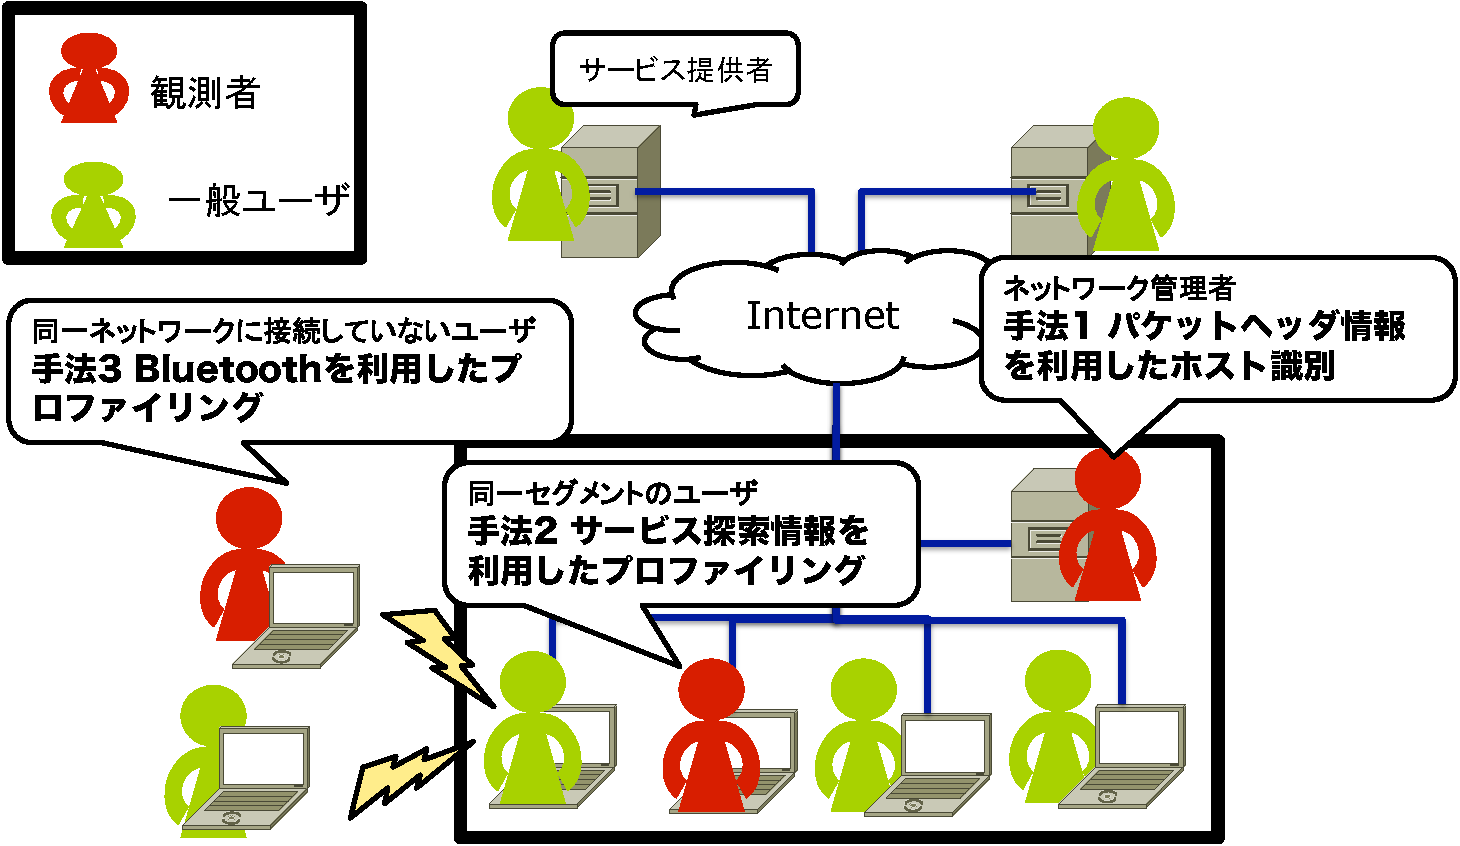
\includegraphics[scale=0.55]{./pdf/zentai}
      \caption{�桼�������ˡ�����ο�}
      \label{fig:zentai}
    \end{center}
\end{figure}


\section{�ͥåȥ�������Ԥȼ�������}
\label{assumption:admin}
�ͥåȥ�������ԤˤȤäƼ������ưפǤ����Τΰ�Ĥˡ��ȥ�ե��å��ǡ�
�����󤲤��롥���������桼�����դ˼��̤Ǥ��롤�ѥ��åȤΥڥ�������
��MAC���ɥ쥹�ʤɤϥͥåȥ���Υݥꥷ�乽���ˤ�äƼ����Ǥ��ʤ���礬
���롥�����ǡ��ѥ��åȤΥإå�����˾��������ơ��ѥ��åȤΥإå������
�ߤ��顤�ۥ��Ȥ����ꤹ���ˡ����Ƥ��롥

\subsection{����}
\label{assumption:admin:premise}
%3) ���ξ����ɤΤ褦�����Ѥ���ȤɤΤ褦�ʷ�̤�������Τ�
�ѥ��åȥإå���������ˤ��ץ饤�Х��ζ��Ҥ˴ؤ����ˡ������ˤĤ���
�Ҥ٤롥�ѥ��åȤξ�����������ͥåȥ�������Ԥϡ��ͥåȥ���Υ�
�ꥷ��ͳ������Ǥ���ISP��ͥåȥ�������Ԥ����ꤹ�롥
��\ref{fig:packet_model}�˼����褦�ˡ������Ԥ��ѥ��åȤΥإå�������
�����뵡��򡤥ͥåȥ����������������֤��뤳�Ȥˤ�äơ��ͥåȥ
���ȥ�ե��å���������롥�ͥåȥ�������ϰ�ս�Τ߳��˽Ф������¸
�ߤ���Ʊ���ͥåȥ���ˤ����ƥ桼����ȯ������ѥ��åȤ�ɬ�����ε����
�̲᤹���ΤȤ��롥

\begin{figure}
    \begin{center}
      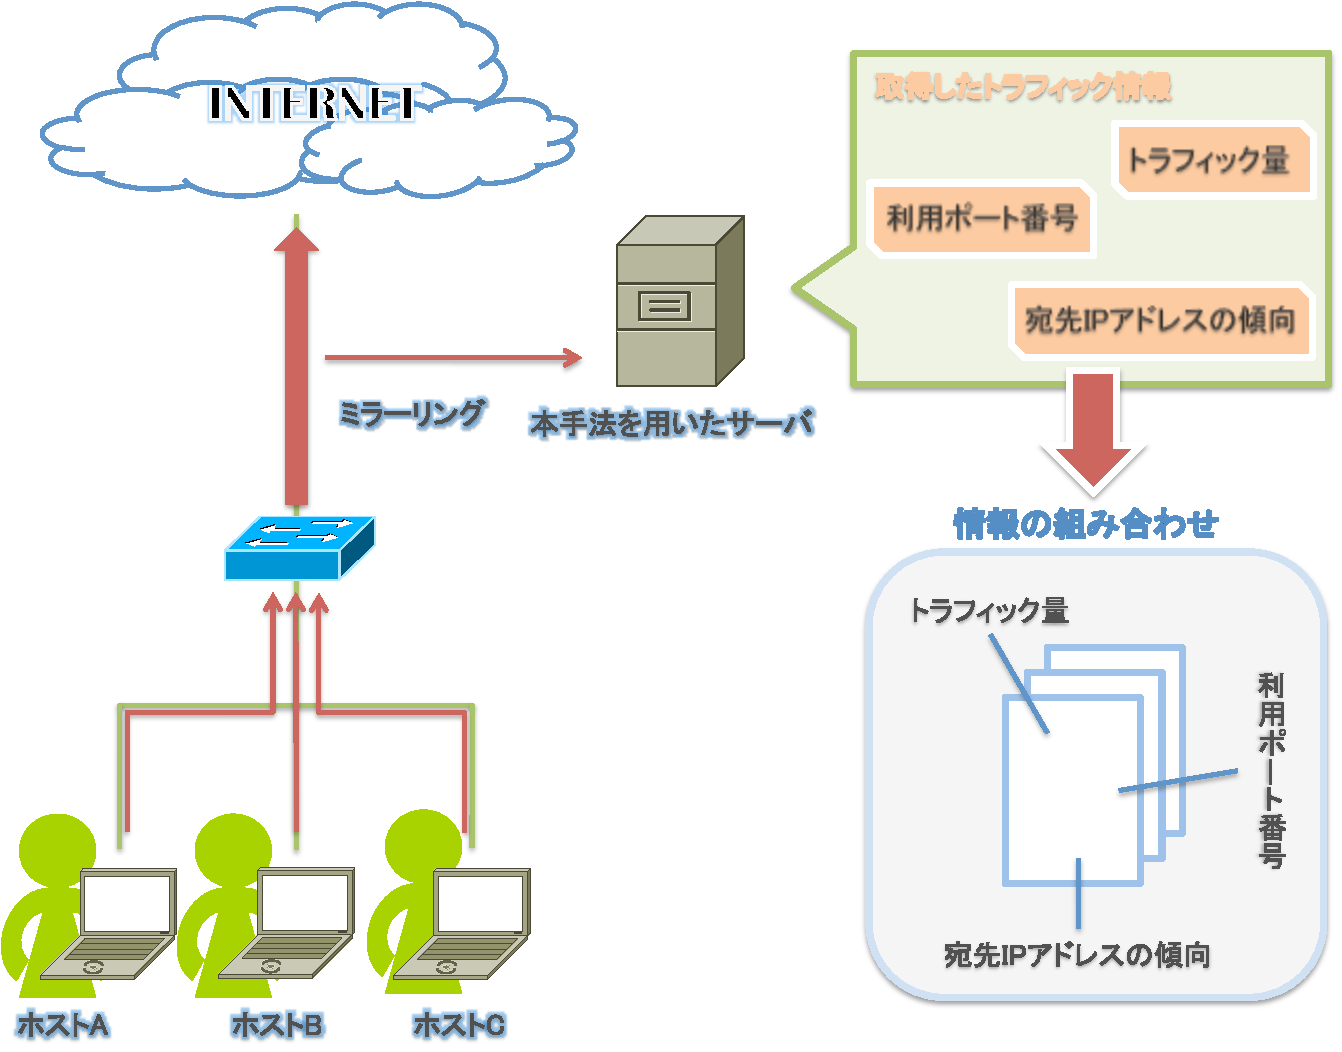
\includegraphics[scale=0.55]{./pdf/packet_model}
      \caption{�ѥ��åȥإå�����μ��������ƥ�γ���}
      \label{fig:packet_model}
    \end{center}
\end{figure}


\subsection{�ѥ��åȤΥإå�����}
\label{assumption:pakcet}
% 1) �ʤ����ξ�������ܤ�����
�ѥ��åȤΥإå�����ϥͥåȥ�����ή���ȥ�ե��å����¬�������
�Ǽ������뤳�Ȥ��Ǥ��뤬���ڥ������ɤ�ޤ����������硤�桼���θĿ�
�����̩�ܤʴؤ�꤬���뤿��桼����Ʊ�դ�ɬ�פǤ��롥���������ͥåȥ
�������Ԥ����ͥåȥ���Ӱ�����桤�ͥåȥ������̿������פ�ȥ��
�ɤ����Ѥ�������硤�ѥ��åȤ�������뤿������ƤΥ桼����Ʊ�դ����뤳
�ȤϺ���Ǥ��롥���Τ��ᡤ�ڥ������ɤϱ��������˥إå�����Τߤǥͥå�
������ΤΥȥ�ե��å�����������ˡ����Ƥ���Ƥ���\cite{blinc:2005}��
�����ǽҤ٤Ƥ���ѥ��åȤΥإå�����������衤ȯ����IP���ɥ쥹���ݡ���
�ֹ桤�ץ��ȥ����ؤ������������ѥ��åȤΥإå��������������ˡ����
�桼���Υץ饤�Х��򶼤����ʤ��Ȥ��Ǹ��Ǥ��ʤ���
%2)�ʤ����β������Ƥ���˻�ä���

�ƥ桼���Ϥ��줾������Ѿ����˱�������ħŪ�ʥѥ��åȤ����������Ƥ��롥
�إå����󤫤�ϡ������衦ȯ����IP���ɥ쥹���ݡ����ֹ椫����Ѥ��Ƥ���
�����ӥ������ץꥱ�������λ������٤ξ��󤬼����Ǥ��롥�����ơ�����
��IP���ɥ쥹����ϥ桼�����̿����ξ����İ���ǽ�Ǥ��롥����ˤ�äơ�
�����桼���ϤɤΤ褦�ʥۥ��Ȥ��̿����뷹�������뤫���İ��Ǥ��롥¾�ˤ�
�إå�����Τߤ�OS���¬����Passive Finger
printing\cite{passivefinger:2010}�����Ѥ��뤳�Ȥǡ��ۥ��Ȥμ������ǤȤ�
�롥���Τ褦�ˡ�¿���ε��Ѥ��Ȥ߹�碌�뤳�Ȥˤ�äơ��ۥ��Ȥ˴ؤ����
������ѤǤ��롥�������Ѥ���������Ȥ˥ۥ��Ȥ�����򤹤��ˡ����Ƥ��롥
��³���٤�¿���ۥ��Ȥ䡤��ư���ε�ư���ץ��ȥ����ž���̤�������뤳��
�ǡ��ۥ��Ȥ������������뷹���Τ��륵���Ȥ䡤���Ѥ��Ƥ��륢�ץꥱ������
�󡤥ͥåȥ����Ǥε�ư���¬�Ǥ��롥

% 4) ���줬�ɤΤ褦�ʥ���ѥ��Ȥ�ï��Ϳ����Τ����μ�ˡ�ˤ�äƥ桼����
% �ץ��ե����뤬�����Ǥ���С��ͥåȥ�������Ԥ�ͥåȥ����ή���
% �ȥ�ե��å�����μ谷�������桼����Ʊ�դȤ��ä��ץ饤�Х�����θ����
% �ݥꥷ���θ���ʤ���Фʤ�ʤ����ޤ������̥桼���ϡ��Ŀͤ˴ؤ�����
% ���Τ餺�˾��ȯ�����Ƥ��ꡤ�ͥåȥ�������Ԥʤɤˤ�äƥ桼���Υ�
% �饤�Х�����������Ƥ����ǽ�������롥

\subsection{�ۥ��ȼ��̤ˤ��Ĵ��}
\label{assumption:used}

�ºݤ˥ѥ��åȤΥإå��˴ޤޤ����󤬼������ǤȤ�������Ω�ĤΤ��Ȥ�����
��Ĵ��Ĵ����Ԥä����ʲ��˸Ŀͤ���������ѤǤ�������Ҥ٤롥

\subsubsection{�Ŀͤ���������ѤǤ������}

\begin{itemize}
\item{\bf ������IP���ɥ쥹�ȥݡ����ֹ���Ȥ߹�碌}\\
�������ݡ����ֹ��IP���ɥ쥹�δط������ܤ���Ĵ����Ԥä���
���η�̡��������ǤȤ������ꤷ�Ƥ���IP�ݡ����ֹ�ˤ�뼱�̤Ϻ���Ǥ��뤳��
��Ƚ����������\ref{fig:userA_ipport}�˥ۥ���A��������IP���ɥ쥹���ݡ���
�ֹ桤��\ref{fig:userB_ipport}�˥桼��B��������IP���ɥ쥹���ݡ��Ȥ�
����X����IP���ɥ쥹��Y�����ݡ����ֹ�򼨤���

\begin{figure}
    \begin{center}
      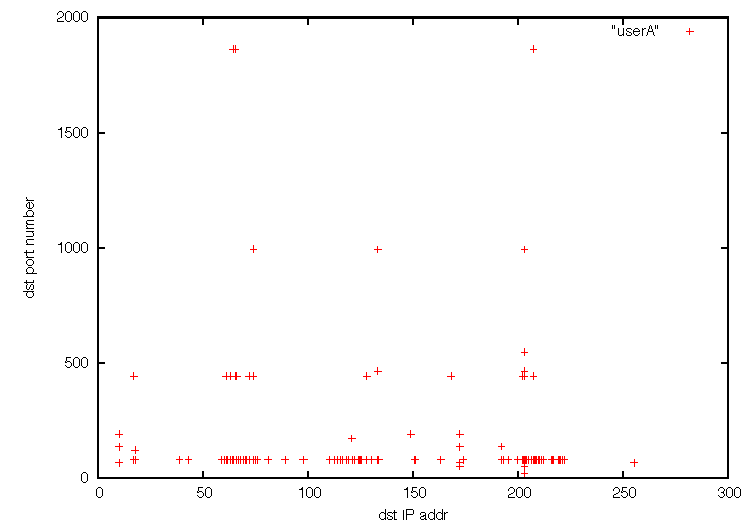
\includegraphics[scale=1.06]{./pdf/userA_ipport}
     \caption{�ۥ���A��������IP���ɥ쥹���ݡ����ֹ�}
     \label{fig:userA_ipport}
    \end{center}
\end{figure}

\begin{figure}
    \begin{center}
      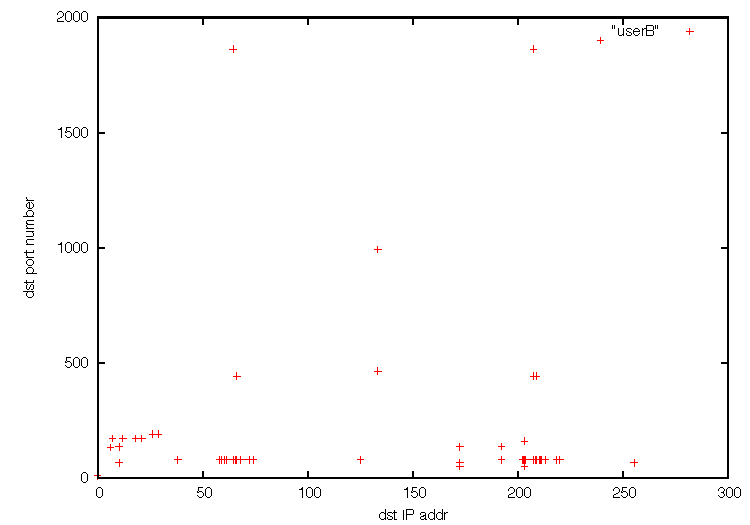
\includegraphics[scale=1.06]{./pdf/userB_ipport}
     \caption{�桼��B��������IP���ɥ쥹���ݡ����ֹ�}
     \label{fig:userB_ipport}
    \end{center}
\end{figure}

����Ĥοޤ���ۥ���A��B�����Τʺ��ۤ򸫤Ĥ��뤳�Ȥ��Ǥ��ʤ��ä�������
����SSH��IMAP��������ʤɡ��ץ��ȥ������³��IP���ɥ쥹�ˤ�äƤϡ��ۥ�
�Ȥ��Ȥ���ħ�����뤳�Ȥ��Ǥ��������Τ��Ȥ��顤������IP���ɥ쥹���ݡ���
�ֹ���Ȥ߹�碌�ϥݡ����ֹ�ˤ�äƤϥ桼���μ������ǤȤ��Ƥ����ѤǤ���
�Ȥ��������˻�ä����ۥ��ȼ��̤����ѤǤ���ץ��ȥ���ϡ�IMAP��SSH��VPN��
�ɤ��󤲤��롥

\item{\bf ȯ�����ݡ����ֹ�}\\
  ��OS���Ȥ�ȯ�����ݡ����ֹ�ϰۤʤꡤ��ħ�������ǽ�������롥���Τ��ᡤ
  ȯ�����ݡ����ֹ�����Ѥ���Ӥ��롥���η�̤��\ref{fig:port_src}�˼�
  ������\ref{fig:port_src}��MacOSX��Windows XP��ȯ�����ݡ����ֹ�����
  ������硤�ưפ˺���ȯ�����뤳�Ȥ��Ǥ��롥Windows XP��MacOSX�򤵤��
  Ĺ��Ū�˴�¬��������Ʊ���������ݡ����ֹ�����Ѥ���뤳�ȤϤʤ��ä���
  ����� ��OS���Ȥ������������ѥݡ��Ȥη������㤦����Ǥ��롥�Ĥޤꡤ��
  �����ݡ����ֹ��������뤳�Ȥ�OS���¬�Ǥ��롥¾OS���¬������硤ȯ
  �����ݡ����ֹ�����Ѥ������ڷ�̤�ɽ\ref{tb:src_portos}�ˤޤȤ�롥��
  �ʾ�Τ��Ȥ��顤IP���ɥ쥹���������ݡ����ֹ�ϼ������ǤȤ������Ѥ���
  ���ȤϤǤ��ʤ������������ݡ����ֹ�����뤳�Ȥ�OS��ʬ�ह�뤳�Ȥ��Ǥ�
  �롥

\begin{figure}
    \begin{center}
      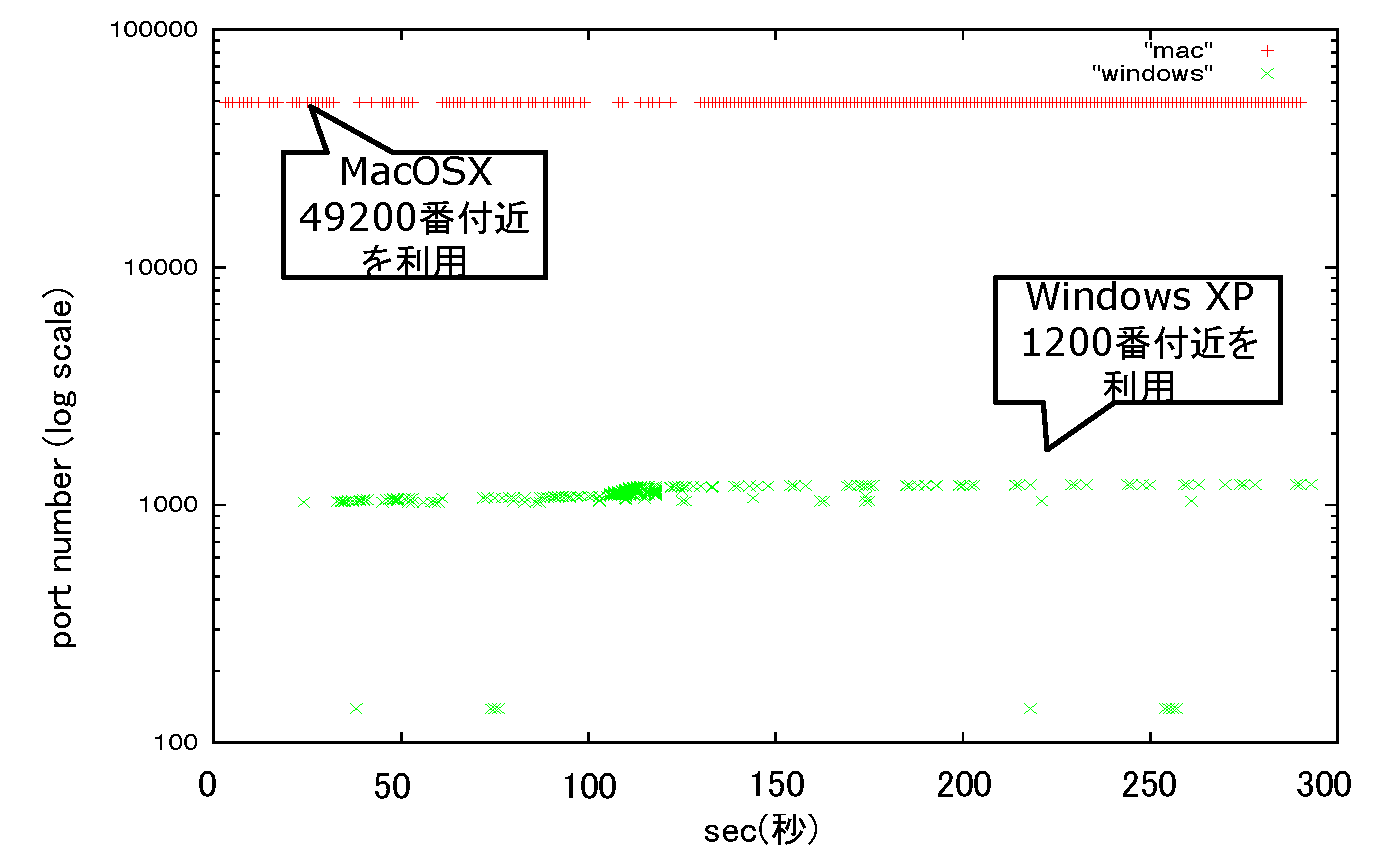
\includegraphics[scale=0.70]{./pdf/src_port}
     \caption{MacOSX��WindowsXP�������������ݡ����ֹ�}
     \label{fig:port_src}
    \end{center}
\end{figure}

\begin{table}
\caption{OS������ȯ�����ݡ���}
\label{tb:src_portos}
\begin{center}
\begin{tabular}{|c||c|}
\hline
OS&ȯ�����ݡ���\\
\hline 
FreeBSD&49152-65535\\
Ubuntu&32768-61000\\
Windows XP&1024-5000\\
Windows Vista&49152-65535\\
MacOSX&49152-65535\\
\hline
\end{tabular}
\end{center}
\end{table}

\item{\bf �ѥ��åȤ�ȯ�������ߥ�}\\
  ���ۥ��Ȥμ��̤ˤ����ꡤ�ǽ�ε�ư���֤����ʬ�δ֥ѥ��åȤΥإå���
  ����¬���뤳�Ȥǥۥ��Ȥ���̤����ꤹ�뤳�Ȥ��Ǥ���Ȥ��������Ω��
  �����ºݤˡ��ۥ��Ȥ�OS�䥹�����ȥ��åפ���Ͽ���Ƥ��륢�ץꥱ�������
  ����ư����Ω���夬�뤿�ᡤ�桼���Υѥ��åȤ�ȯ�������ߥ󥰤���ۥ���
  ���̤Ǥ����ǽ�������롥�ۥ��Ȥˤ�äƤϡ����Ѥ��Ƥ��륢�ץꥱ������
  ��䥵���ӥ��ʤ��͡�����ħ�����뤿�ᡤ�ƥۥ��Ȥ�ȯ������ѥ��åȤΥ�
  ���ߥ󥰤������ǤȤ������ѤǤ��벾�ꤷ���������ǡ�OS����ư���Ƥ���
  �桼�������򤹤�ޤǤΥ����ߥ󥰤˾��������ơ��Ŀͺ����Ф뤫��Ĵ��
  �򤷤��������ߥ󥰤��������Ȥ��ơ��ۥ��Ȥ�IP���ɥ쥹����Ϳ����Ƥ�
  ����2ʬ�֤ξ����Ĵ�����롥���������ѥ��åȤμ��������ߥ󥰤ϥͥåȥ
  ���ˤ�äư�¸���뤿�ᡤƱ���ͥåȥ����Ǽ�������Ȥ������Τ��
  �ѥ��åȤΥȥ�ե��å�������Ԥä��������ߥ󥰼����ˤ����ơ��ɤ�����
  ������ǧ����붦�̤Υǡ����Ǥ���Τ�������������ºݤ�7��OS�򷫤���
  ���ƺƵ�ư
  ��Ԥ���IP���ɥ쥹����Ϳ�����ǽ��2ʬ�֤Υ����ߥ󥰤����������\\
  �������MacOSX version 1.6��Windows Vista��OS���оݤȤ������꡼�󥤥�
  ���ȡ��뤷�����֤Ǹ��ڤ�Ԥä����ޤ���MacOSX�η�̤�
  ��\ref{fig:start_up_mac}�˼�����X����IP���ɥ쥹����Ϳ����Ƥ���ηв�
  ���֤Ǥ��ꡤY�����Ƶ�ư����Ǥ��롥����դ����ϡ��ۥ��Ȥ��ѥ��åȤ�ȯ
  �������ݤ�������롥���ˡ�Windows Vista�ξ��
  �Υ����ߥ󥰤��\ref{fig:start_up_win}�˼�����

\begin{figure}
    \begin{center}
      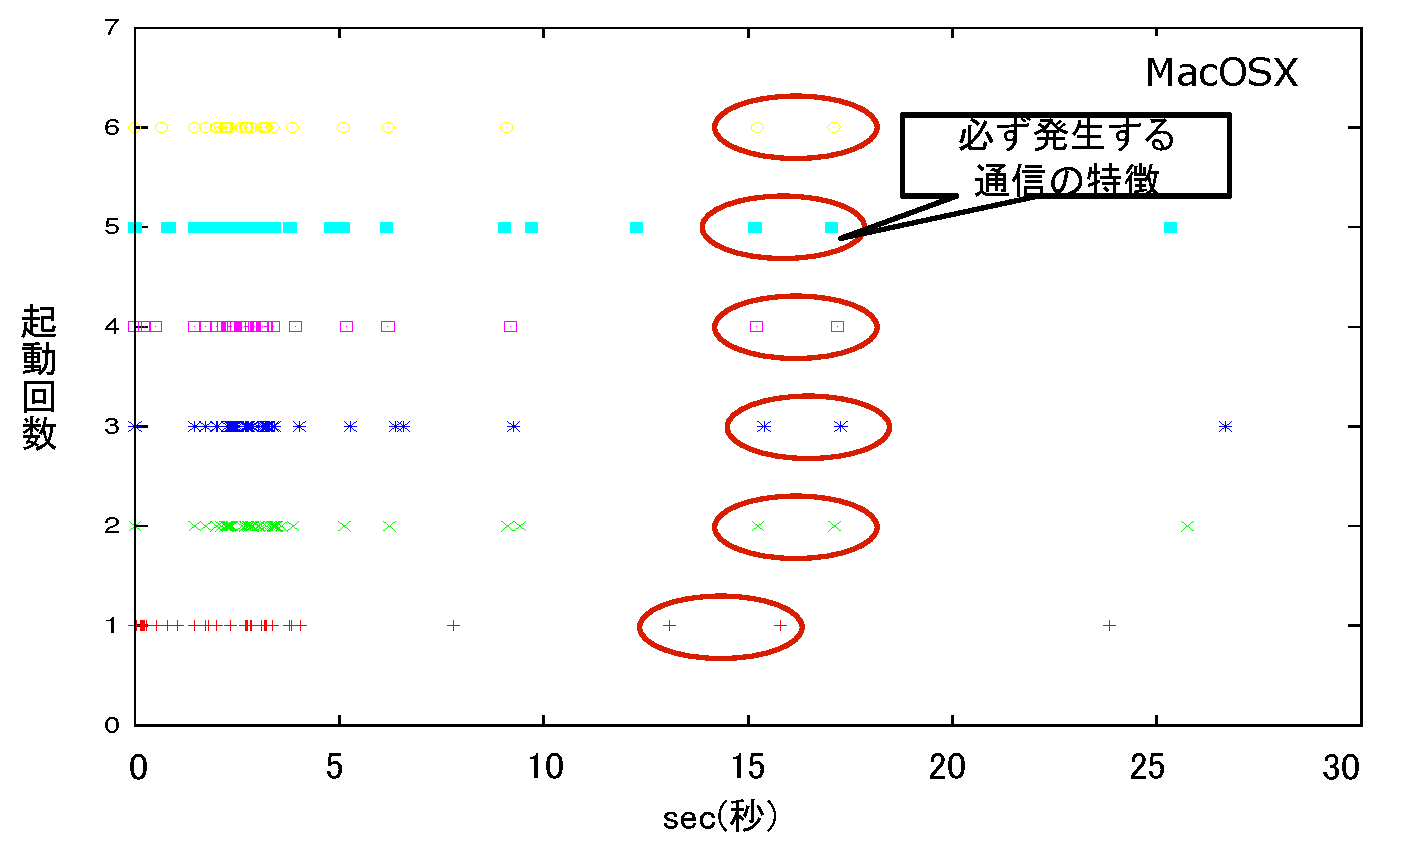
\includegraphics[scale=0.65]{./pdf/stup_mac2}
      \caption{MacOSX�ε�ư���Υѥ��åȤ�ȯ�������ߥ�}
     \label{fig:start_up_mac}
    \end{center}
\end{figure}

\begin{figure}
    \begin{center}
      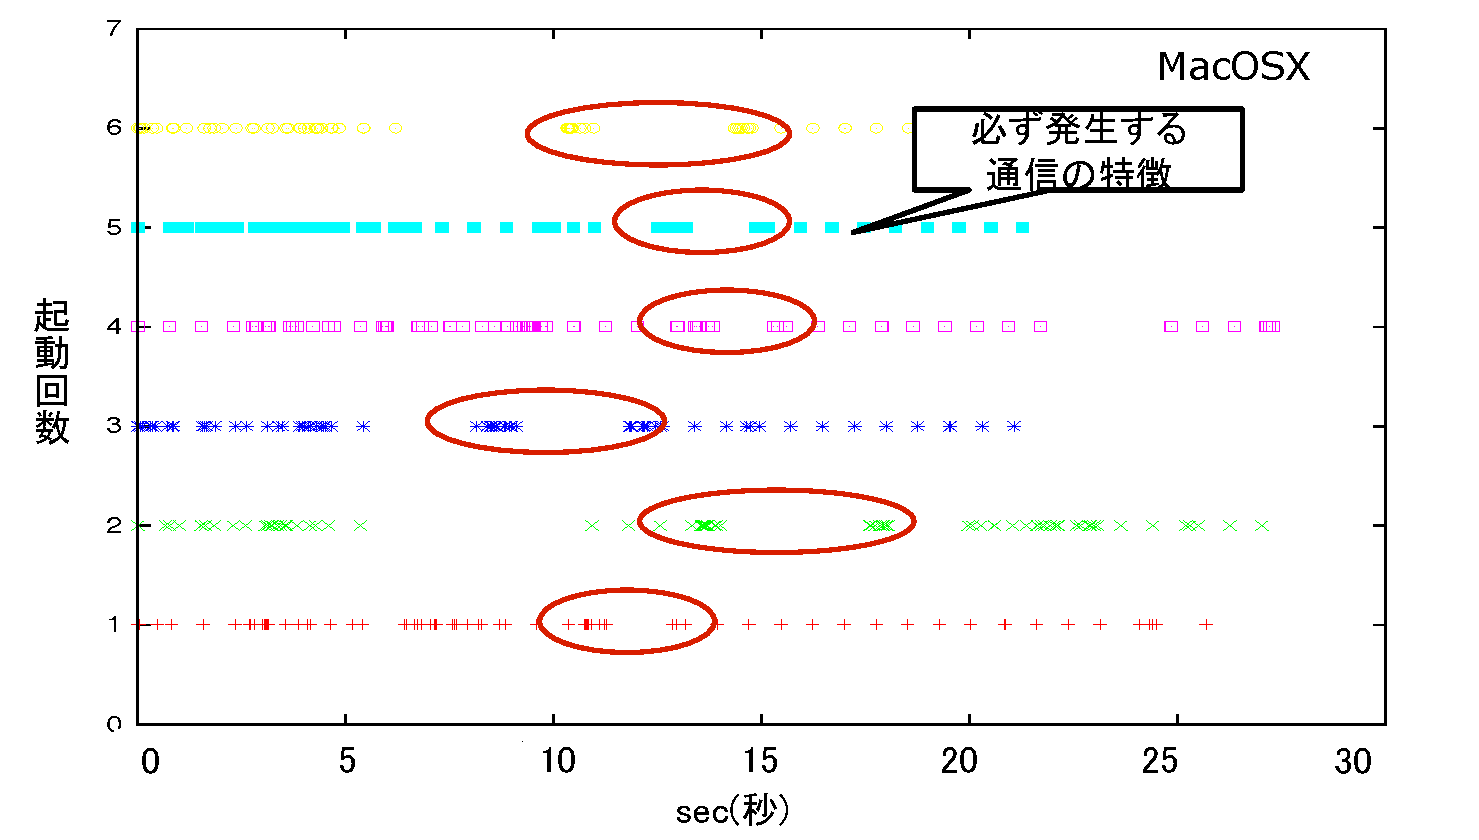
\includegraphics[scale=0.65]{./pdf/stup_win2}
      \caption{Windows Vista�ε�ư���Υѥ��åȤ�ȯ�������ߥ�}
      \label{fig:start_up_win}
    \end{center}
\end{figure}

��MacOSX�˴ؤ��Ƥϡ��ǽ�ο�ʬ�֤ˤ����ư�����̿��򷫤��֤�������������
���Ū����ħ�νФ䤹����̤Ǥ��뤳�Ȥ�ʬ���롥�äˡ���ư���Ƥ���1�ø夫
��2�ø夬��ħŪ�Ǥ��ꡤ���Υ����ߥ󥰤�������뤳�ȤǼ������ǤȤ�������
�Ǥ����ǽ��������ȿ�¬�Ǥ��롥������Ф���Windows�ξ���IP���ɥ쥹��
��Ϳ����Ƥ�������ä�Ϣ³Ū���̿���¿�����ᡤWindows��MacOSX ���礭��
�㤤���Ф��ȸ����롥�ä˸����ʤΤ�MAC OS��Ʊ����1�ä���2�äε�ư�Ǥ��롥
���ε�ư�δֳ֤κ�
�����Ѥ��뤳�Ȥˤ�äơ�OS�����꤬��ǽ�Ǥ���ȸ����롥\\
�����ˡ��ƥѥ��åȤΥץ��ȥ���ȥݡ����ֹ�򼨤�����Ĥ�OS�Υѥ��å���
�������ߥ󥰤�����ʬ���ƹ��˾ܤ������Ϥ�������դ�
��\ref{fig:port_mac}�ȿ�\ref{fig:port_win}�Ǥ��롥�ץ��ȥ��뤴�Ȥ�ʬ��
�����ݡ����ֹ��̤�ɽ����������\ref{fig:port_mac}����\ref{fig:port_win}��X����IP���ɥ쥹��
��Ϳ����Ƥ���λ��֤��Ф��ơ�Y���ϥݡ����ֹ��ؤ��Ƥ��롥�ޤ������ˤ��
��UDP��TCP��ICMP��3����ˤ�ä�ʬ�ष�Ƥ��롥����ˤ��
�ơ�mDNS��SMB��DNS�ʤɤ��̿���¿����¬�Ǥ��롥��������ѥ��åȤζ��̹�
��������롥¾�ˤ⡤����ư���㤦�ѥ��åȤ��ӽ����롥�㤨
�С�LDAP��NetBIOS�ʤɡ�
�ͥåȥ����������ۥ��ȷ��˺��Ѥ����ѥ��åȤ��ӽ����롥

\begin{figure}
    \begin{center}
      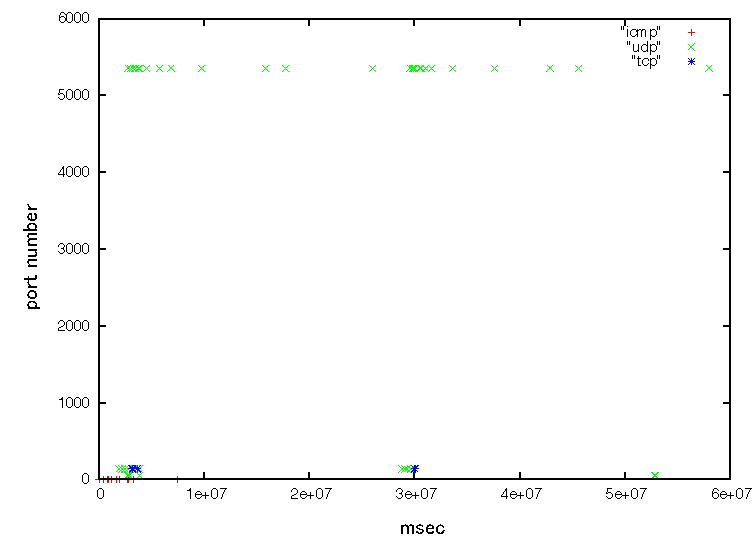
\includegraphics[scale=1.00]{./pdf/mac_port}
      \caption{MacOSX�Υݡ����ֹ�ȥץ��ȥ����̥ѥ��åȤ�ȯ�������ߥ�}
      \label{fig:port_mac}
    \end{center}
\end{figure}

\begin{figure}
    \begin{center}
      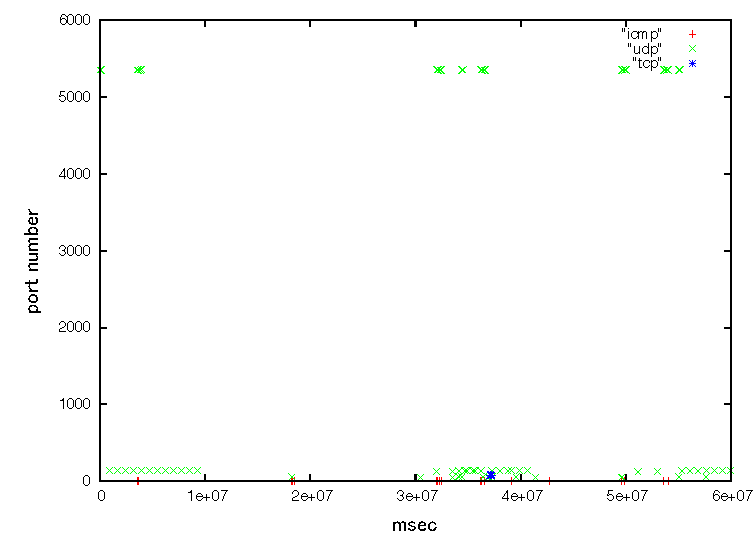
\includegraphics[scale=1.00]{./pdf/win_port}
      \caption{Windows Vista�Υݡ����ֹ�ȥץ��ȥ����̥ѥ��åȤ�ȯ�������ߥ�}
      \label{fig:port_win}
    \end{center}
\end{figure}

�����������Ȥ��ơ��ͥåȥ�������Ԥ����ꤷ�Ƥ��뤿
�ᡤMSND��NetBIOS�ʤɤΥޥ�����㥹�Ȥ�֥����ɥ��㥹�Ȥ��̿�������Ǥ�
�ʤ���ǽ�������롥�����ǡ��ޥ�����㥹�Ȥ�֥����ɥ��㥹�Ȥ���������
�ϡ������ξ����������뤳�Ȥ�����Ǥ��롥�äˡ�MacOSX���ưפ�ȯ����
������\ref{fig:start_up_mac}�ǤΥۥ��Ȥ���ħ�ϥޥ�����㥹�Ȥ�
���뤿�ᡤ�����ߥ󥰤Τߤǥۥ��Ȥ��̤��뤳�ȤΤϺ���Ǥ��롥MacOSX��Ʊ����mDNS��SMB�Υѥ��åȤ�¿����������Ƥ��뤬��Microsoft�ҤΥ����Ф��Ф���HTTP�̿��򤷤Ƥ��뤿�ᡤTCP�Υѥ��åȤ�ȯ�����륿���ߥ󥰤����ܤ��뤳�Ȥ��ưפ�ȯ���Ǥ��롥\\
�������ǡ��ѥ��åȤ�ȯ���Υ����ߥ󥰤�ư���Ƥ���ο����ø�˾�������
�Ƥ롥�ºݤ˥��ץꥱ������󤬵�ư������֤��¬�����Ȥ�����IP���ɥ쥹
����Ϳ����Ƥ�����60�ø�˻�������Ͽ���Ƥ��륢�ץꥱ������󤬵�ư����
�������ᡤ60�ø�ε�ư�����ܤ�����60�ä���120�äδ֤˥ѥ��åȤ�ȯ��������
����硤�ʤ�餫�Υ��ץꥱ������󤬼�ư��ư�����ꤵ��Ƥ����ǽ������
�롥��\ref{fig:port_mac}�ˤ���ޤ�TCP��NetBIOS���å���󥵡��ӥ��Ǥ��ꡤ
���̻ҤȤ��ƤϽ�������롥���Υѥ��åȤ����������ߥ󥰤ȥץ��ȥ������
�Ѥ��ơ���ư��ư�����ꤵ��Ƥ��ʤ��ۥ��Ȥ����ꤷ��
����ۥ��Ȥ�ʬ��Ǥ��롥\\
�����ˡ���ư��ư�����ꤷ�Ƥ��륢�ץꥱ�����������ꤹ��ɬ�פ����뤬��
����¿���Υ��ץꥱ������󤬤��뤿�᤹�٤Ƥ����夹�뤳�Ȥ��Բ�ǽ��
���롥�����ǡ���������ѼԤ����Ū¿��IMAP��MSN��å��󥸥���оݤȤ��Ƽ��夲�롥\\
��IMAP��MSN��å��󥸥�����Ѥ���ݡ��Ȥ����ꤵ��Ƥ��ꡤimap��993�֤�
����MSN��1864�֤Ǥ��롥���Υݡ����ֹ椫���������ѥ��åȤΥȥ�ե��å�
�̤���Ŀͤμ������ǤȤ������ѤǤ����ǽ�����󤲤��롥�㤨�С�MSN���
���󥸥�ʤɤ�Ϣ����Υ桼���Υꥹ�Ȥ��ݻ����Ƥ��뤿�ᡤ���Υꥹ�Ȥ��
��������ɤ��ʤ���Фʤ�ʤ�����������Ѥ��뤳�Ȥˤ�äơ��ɤ����٥ꥹ
�Ȥ���Ͽ���Ƥ���Τ����¬�Ǥ��롥Ʊ�ͤˡ�IMAP�����Ѥ��뤿��ˤϥ�����
����ե������᡼��Υꥹ�Ȥ����������ɤ���ɬ�פ����롥
���Υȥ�ե��å��̤���桼���μ������ǤȤ������Ѥ��뤳�Ȥ��Ǥ��롥\\
���嵭����ˡ�ϥۥ��ȵ�ư���ο�ʬ�֤ε�ư���Ȥ˿�¬��ԤäƤ��뤿�ᡤ
�ͥåȥ���˻��ä���桼�����Ÿ�����Ȥ������֤��鵯ư������������
�ڥ�ɤ⤷���ϥϥ��ѥ͡�����󤫤������������ˤ�äơ���������٤�����
��������٤�������礭���Ѳ����롥���ε�ư���ٻ߾��֤������������Ƚ��
������ˡ�˥ѥ��åȤ�ȯ�������ߥ󥰤������ǤȤ������Ѥ��뤳�Ȥ��Ǥ��롥
�����μ�ˡ���Ѥ��ơ�IP���ɥ쥹����Ϳ���줿���֤���ѥ��å�ȯ���Υ���
�ߥ󥰤��¬���뤳�Ȥǡ��ͥåȥ������³�����ۥ��Ȥ�����ư�����Τ���
���줷���Τ����ưפ�Ƚ�̤��뤳�Ȥ��Ǥ��롥��\ref{fig:up_or_sus}��IP����
�쥹����Ϳ����Ƥ���Υۥ��Ȥε�ư����������Υѥ��åȤ����������ߥ�
����ӤǤ��롥X����IP���ɥ쥹����Ϳ����Ƥ���λ��֤��Ф��ơ�Y���ϵ�ư
���ε�ư��������ε�ư�Ȥ��ä���٥�Ǥ��롥

\begin{figure}
    \begin{center}
      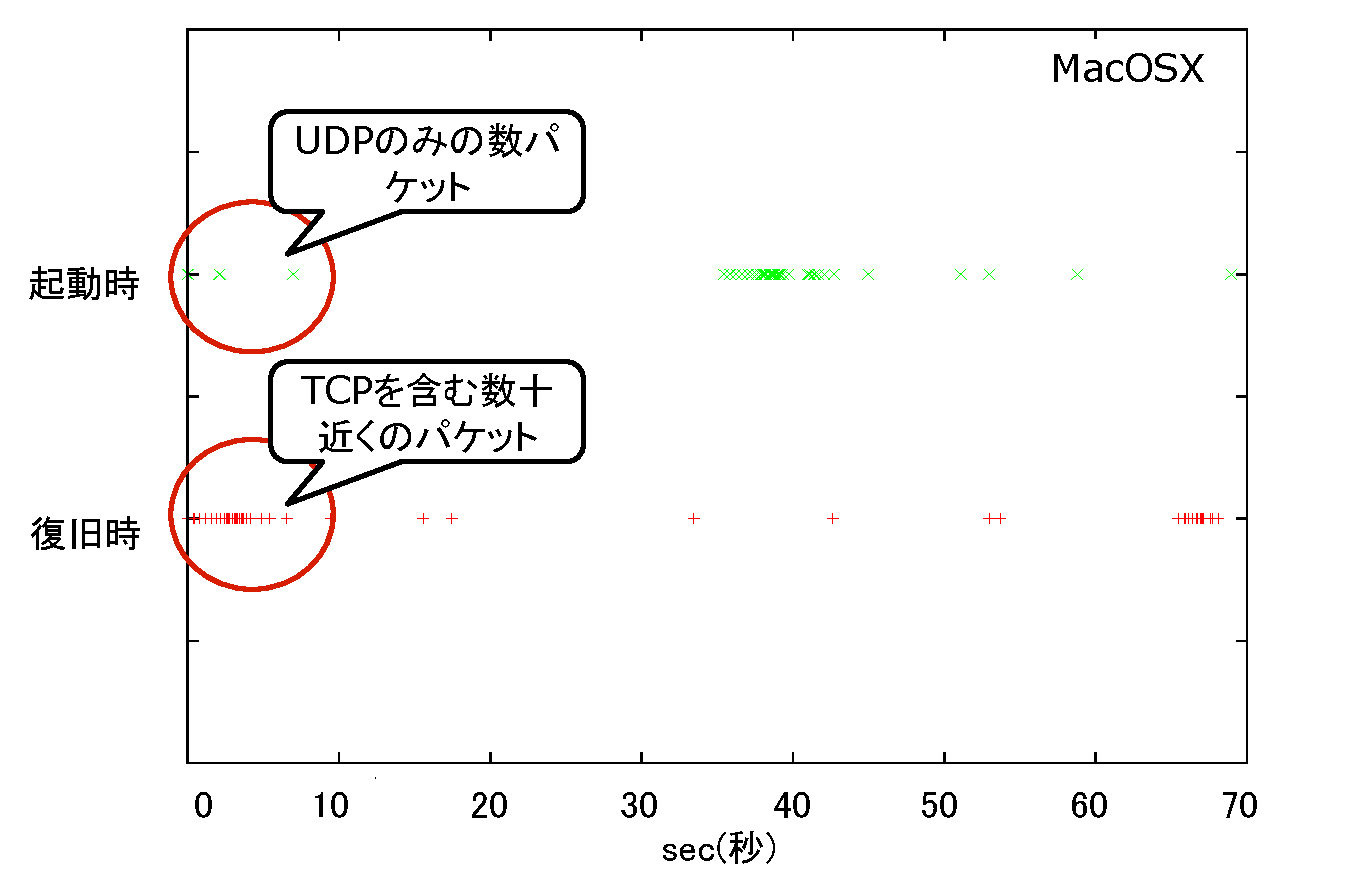
\includegraphics[scale=0.70]{./pdf/startup_suspend}
      \caption{��ư����������ˤ�����ѥ��åȤ�ȯ�������ߥ󥰤����}
      \label{fig:up_or_sus}
    \end{center}
\end{figure}


��Ʊ�����꡼�󥤥󥹥ȡ�������Ѥ���MacOSX�Ǥ���Τ��Ф��ơ����Τʺ���
���ޤ줿����������Ÿ�������Ƥ�����֤���ε�ư������٤ơ��᤯�ۥ���
�����Ѥ��뤳�Ȥ��Ǥ��롥�����ڥ�ɤ⤷���ϥϥ��ѥ͡������ϥ��ץꥱ��
������OS��ɬ�פʵ�ǽ��Ω���夲�Ƥ�����֤ǹԤ��뤿�ᤢ�롥�ޤ�����
��ο����äε�ư��Ʊ��OS�Ǥ���ФɤΥۥ��ȤǤ�Ʊ���Ǥ��뤿�ᡤ��ư����
���äǰۤʤ��ư�򤷤���硤
�ٻ߾��֤������줷����Ƚ�Ǥ��뤳�Ȥ��Ǥ��롥\\
��OS���ٻ߾��֤������줷�����ϡ��Ŀ�����ν��פʼ������ǤȤʤ롥OS��
���Ѥ���ȯ�����ݡ����ֹ�ϰۤʤ뤳�Ȥ����Ҥ����̤�Ǥ��롥�ٻ߾��֤���
���줷����硤ȯ�����ݡ��Ȥ�Ϣ³�����ݡ����ֹ�����Ѥ��롥�Ĥޤꡤ�ٻ�
�������Ѥ���Ƥ���ȯ�����ݡ��Ȥο�����Υݡ����ֹ�����Ѥ��뷹�������롥
�����ǥۥ��Ȥ����Ѥ��Ƥ���Ǹ��ȯ�����ݡ����ֹ����¸���뤳�Ȥˤ�äơ�
���Υۥ��Ȥ�Ʊ���ͥåȥ��������줷����硤�ۥ��Ȥμ������ǤȤʤ���
�롥�����������٥ۥ��Ȥ�Ƶ�ư�����ȯ�����ݡ��ȤϽ���ͤ���뤿�ᡤ��
�����ݡ����ֹ�����Ѥ������̼�ˡ�����줷���ۥ��ȤˤΤߤ����Ѥ��뤳�Ȥ�
�Ǥ��롥

\item{\bf �ۥ��Ȥ����Ѥ��륵���ӥ�}\\
  ���桼�������Ѥ��������襢�ɥ쥹�䡤�ݡ����ֹ椫��ʬ���륵���ӥ���
  �����ǤȤ��롥�㤨�С�Web�����ӥ�����Ѥ����硤���Ѥ��Ƥ���Web����
  �Ȥˤ�äƥ桼����ץ��ե�����󥰤Ǥ��롥�����ӥ����������٤䷹����
  �桼�����Ȥ˺��ۤ��뤿�ᡤ�桼���μ������ǤȤ��Ƥ�ͭ���Ǥ��롥���Τ�
  �ᡤWeb���ץꥱ��������SNS�����Ѥ������٤�����Ӥ�ƥ桼�����Ȥ�Ĵ
  �٤뤳�Ȥˤ�ä��������桼����Ĵ�����롥�㤨
  �С�mixi\cite{mixi:2009}��Twitter\cite{twitter:2009}�ʤɤ˥���������
  ������Ӥ�ֳ֤�ƥ桼�����Ȥ˵�Ͽ���롥�����ϥ桼����ͭ�η����Ǥ���
  ����桼�����̤μ������ǤȤʤ����롥�ޤ����桼���ν�°����ͥåȥ
  ����Mail�����С�Web�����ФؤΥ��������������פǤ��롥�������ܸ���
  �ϳƥ桼���Υ��ץꥱ�������䥵���ӥ����������٤䥢����������ֳ֤�
  �Ѥ��ƥ桼�����̤��롥

\item{\bf ���ѥ��ץꥱ�������}\\
\begin{table}
\caption{�������ǤȤ����оݥġ������}
\label{tb:tools_list}
\begin{center}
\begin{tabular}{|c||c|}
\hline
�оݥġ���&��ʵ�ǽ\\
\hline 
Thunderbird&�᡼�륯�饤����� \\
Outlook&�᡼�륯�饤����� \\
firefox& Web�֥饦�� \\
safari& Web�֥饦�� \\
Omunigraffile&����ġ���\\
Skim&pdf�Խ��ġ���\\
Windows update&OS ���åץǡ��� \\
MacOSX software update&OS ���åץǡ��� \\
GOM player&��ǥ����ץ쥤�� \\
Quick Time&��ǥ����ץ쥤�� \\
VLC media player&��ǥ����ץ쥤�� \\
Windows media player&��ǥ����ץ쥤�� \\
\hline
\end{tabular}
\end{center}
\end{table}
���ۥ��Ȥ����Ѥ��륢�ץꥱ�������ˤ�äƥ桼���Υץ��ե���������ϲ�
ǽ�Ǥ��롥ɽ\ref{tb:tools_list}�˥ۥ��ȼ������ǤȤ����оݥ��ץꥱ������
��򼨤������ˡ�Web���������ʤ����򤫤�桼���ζ�̣ư�����¬��
�롥HTTP�ץ��ȥ����IP���ɥ쥹����³���٤����ѤǤ��롥�ޤ���OS��ư����
��ưŪ�˥��ץꥱ�������Ʊ���˵�ư�����礬���롥���κݤˡ���������
�������Ͽ���뤳�Ȥǥۥ��Ȥ�ʬ�ह�뼱�����ǤȤʤ롥�����μ�������
�����Ѥ��ơ��ۥ��Ȥ�ʬ�ࡤ�ǽ�Ū�ˤϥץ��ե������������롥

\item{\bf �ѥ��åȤΥ�����}\\
  ���ѥ��åȤ�ȯ������������������IP�إå���TCP�إå����Ȥ߹�碌��
  ���Ϥ��뤳�Ȥˤ�äơ��桼����OS������Τ뤳�Ȥ��Ǥ��롥Passive OS
  Fingerprinting�����Ѥ��뤳�Ȥˤ�äƥ桼���ν�ͭ���Ƥ���ۥ��Ȥ��İ�
  ���롥

�ʾ夬�ѥ��åȤΥإå���������Ѥ��ƥۥ��ȼ��̤����ˡ�˺��Ѥ��������
���롥
\subsubsection{�Ŀͤ���������Ѥ�����ʾ���}
\item{\bf DHCP���������Ƥ���IP���ɥ쥹}\\
  ���ͥåȥ���ˤ������̿��Ǥ�IP���ɥ쥹�ϥۥ��Ȥμ������ǤȤ�������
  ����Ƥ��롥IP���ɥ쥹ñ�Τ˾��������Ƥ���硤�ۥ��Ȥ�桼���Ȥ��Ƥ�
  �������ǤȤ�������Ω�ĤΤ������꤬���롥�����ǡ�DHCP�����ФΥ���
  ��2009ǯ7��12��6������7��18��6���ޤǼ�������ʬ�Ϥ�����
  ��\ref{fig:dhcp}��ɮ�Ԥ���°���븦�漼�Υͥåȥ���ˤ�����ۥ���
  ��IP���ɥ쥹���ܤ򼨤�����������IP���ɥ쥹����233���Ф��Ƽ�����
  ��MAC���ɥ쥹����321�Ǥ��ä������Τ�����Ʊ��ȸ�����ۥ��Ȥ�IP����
  �쥹���ܤ�101�󤢤ꡤ�������7���IP���ɥ쥹���Ĥ��Ѥ��ۥ��Ȥ�¸��
  �������Ĥޤꡤ��¬����6���֤ˡ�43\%�Υۥ��Ȥ�IP���ɥ쥹���Ѳ�������
  �ˤʤä���DHCP�����Ф�����塤����IP���ɥ쥹����Ϳ�����ۥ��Ȥˤ�Ʊ
  �����ɥ쥹���꿶���롥�ޤ���Ʊ���ۥ��Ȥ���³���ƥͥåȥ������
  �������Ʊ��IP���ɥ쥹����꿶���롥��\ref{fig:dhcp}�Ǥ�󤲤��
  ��褦�ˡ����٤�IP���ɥ쥹���Ѳ����ʤ��ä��ۥ��Ȥ�130�椢�ä�����������
  ��Ϳ����IP���ɥ쥹���ϰϰʾ�˥ۥ��Ȥ�¸�ߤ�����硤IP���ɥ쥹�ϤĤ�
  �Ѥ�äƤ��ޤ������Τ��ᡤ�ͥåȥ���ˤ����ƥۥ��Ȥ�桼���μ���
  �ˡ�IP���ɥ쥹ñ�ΤǤϼ������ǤȤ������ѤǤ��ʤ���

\begin{figure}
    \begin{center}
      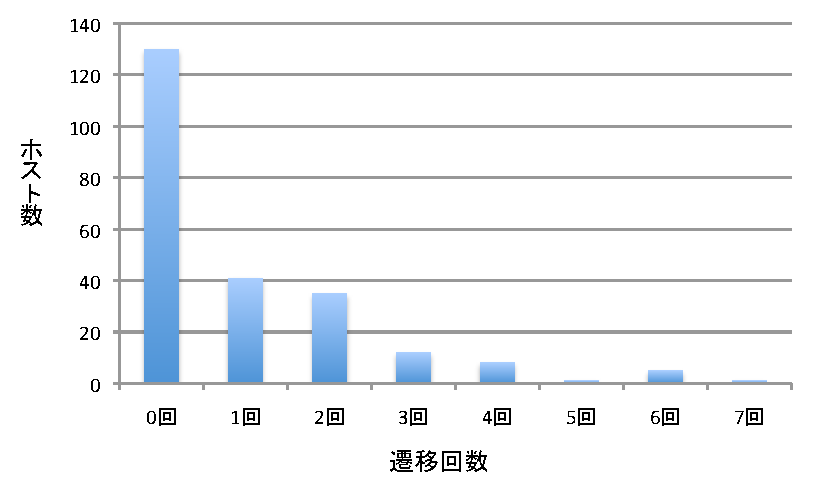
\includegraphics[scale=1.00]{./pdf/dhcp}
      \caption{���֤ˤ�����ۥ��Ȥ�IP���ɥ쥹���ܲ��}
      \label{fig:dhcp}
    \end{center}
\end{figure}




\item{\bf ��ư���֡���³����}\\
���桼�����ۥ��Ȥ�ͥåȥ������³�������֤���³�����Ӥε�§����Ͽ���ơ�
�ܿͤ����转����桼���μ������ǤȤ��롥
�ʹ֤����转����¿���Τ֤줬�����뤬���������İ����뤳�Ȥˤ�äơ��ѥ����������Ǥ����ǽ�������롥
���Τ��ᡤ�桼�����ͥåȥ������³�������٤䤽����³���֤ϥ桼���μ��̤κ����Ȥʤ롥
����˲ä����ܥ����ƥ�ϥۥ��Ȥ�ư���˰��ֺǽ�����Ѥ���ץ��ȥ�����̿������⼱�����ǤȤ��롥
Ĺ��Ū�˥ͥåȥ���ȥ�ե��å�������������桼�����Ȥη�����ʬ����
�뤬��û���֤����ȥ�ե��å��������Ǥ��ʤ����ϥ桼�����Ȥ˺��ۤ򸫤�
����ΤϺ���Ǥ��롥
\item{\bf ��³����}\\
���ͥåȥ������͡��ʰ��֤��ܥ����ƥ�����֤��뤳�Ȥˤ�äơ�
�ۥ��Ȥ���³���֤�������롥
����ˤ�äơ��桼���ι�ư�ϰϤ��İ����뤳�Ȥ���ǽ�Ȥʤ롥
�����������ξ�������ѤǤ��뤫�ϥͥåȥ�������˰�¸���뤿�ᡤ�����
�������ʤ���ΤȤ��롥

\item{\bf TCP SYN �ѥ��åȤ�������IP���ɥ쥹}

\begin{table}
\begin{center}
\caption{������IP���ɥ쥹��̥ꥹ�Ȥ����Ĵ��}
  \vspace{5mm}
\label{tb:dst_IP}
\begin{tabular}{|c|c|c|c|}
\hline
 &�ۥ���A&�ۥ���B&�ۥ���C\\
\hline 
1��&1& 0 & 0\\
\hline 
2��&0& 1 & 0\\
\hline
\end{tabular}
\end{center}
\end{table}

���ۥ��Ȥ�������IP���ɥ쥹�����٤ϥۥ��Ȥ��̤��뤳�Ȥ��Ǥ���Τ�Ĵ��
��Ԥä�������ϡ���³���٤ι⤤������IP���ɥ쥹���5�̤�����������ޤ���
Ʊ���ͥåȥ������Ǥ��̿��Ͻ������롥Ĵ�������ͥåȥ����ɮ�Ԥ���
°���븦�漼�ǤΥͥåȥ���Ǥ��ꡤ�������֤ϡ�2009ǯ6��25��19��45ʬ��
��22��20ʬ�ޤǤǤ��롥���η�̤�ɽ\ref{tb:dst_IP}�˼�����\\
���ƴ��֤ˤ�����Ĵ���оݤΥ桼���ξ��5�̤Υꥹ�Ȥ������ۥ���A��Ʊ
��IP���ɥ쥹1�ġ��ۥ���B�˴ؤ��Ƥ�2�ĸ���줿�����ۥ���C��Ʊ��IP���ɥ�
���������ʤ��ä��������ξ���ϡ��ͥåȥ�������䡤�桼����������
�٤ˤ�äơ������ưפ���ư���Ƥ��ޤ����ᡤ��̤Υꥹ�ȤΤߤǥۥ��ȼ���
���ǤȤ������Ѥ��뤳�ȤϺ���Ǥ��롥

\end{itemize}


\section{Ʊ�쥻�����Ⱦ�Υ桼���ȼ�������}
\label{assumption:same_networkl}
�桼����Ʊ�쥻�����Ȥ���³����ȡ��֥����ɥ��㥹�Ȥ�ޥ�����㥹�Ȥ�
���ä��ͥåȥ�����Τ������������������뤳�Ȥ��Ǥ��롥������Ǥ⡤
�ե����붦ͭ�򤹤�ݤ����Ѥ������ϥۥ������ѼԤ�����Ǥ����ǽ������
�롥¾�ˤ⡤�ۥ��Ȥθ�ͭ�������ǤǤ���MAC���ɥ쥹������Ǥ��롥����
�ǡ�Windows��MacOSX�����Ѥ���Ƥ���mDNS��NetBIOS��MAC���ɥ쥹�ʤɥۥ���
��������Ѥ��뤳�Ȥǡ��ͥåȥ���ˤ�����桼���Υץ饤�Х��򶼤�����ˡ
���󼨤�������\ref{assumption:admin}��Υѥ��åȤΥإå�����ˤ��ۥ�
�Ȥμ��̤Ȱۤʤ����ϡ����˥ۥ��Ȥμ��̤��줿��������Ѥ��뤿�ᡤ�ۥ���
���ѼԤΥץ饤�Х���������������Ǥ��롥

\subsection{����}
����Ȥ��ơ������å��ʤɤ��оݤȤ���桼����NetBIOS��mDNS�Ȥ��ä��ץ���
����μ�����˸���뤳�ȤϤʤ��ͥåȥ�����������ꤹ�롥������������
�桼���ϡ����̥桼���Ǥ��ꡤ�ͥåȥ���ˤ����륵���С��롼����������
����ؤΥ����������¤Ϥʤ���ΤȤ��롥�ޤ���̵��LAN�Ǥ���Хץ��ߥ�����
�����⡼�ɤ����Ѥ��ơ�Ʊ�������ͥ����³���Ƥ�����������Ǥ��뤬��
����Ϥ��ξ������ꤻ����ͭ���ͥåȥ�������Ѥ����Ķ������ꤹ�롥
��\ref{fig:share_model}�ˤ��γ��׿ޤ򼨤���

\begin{figure}
    \begin{center}
      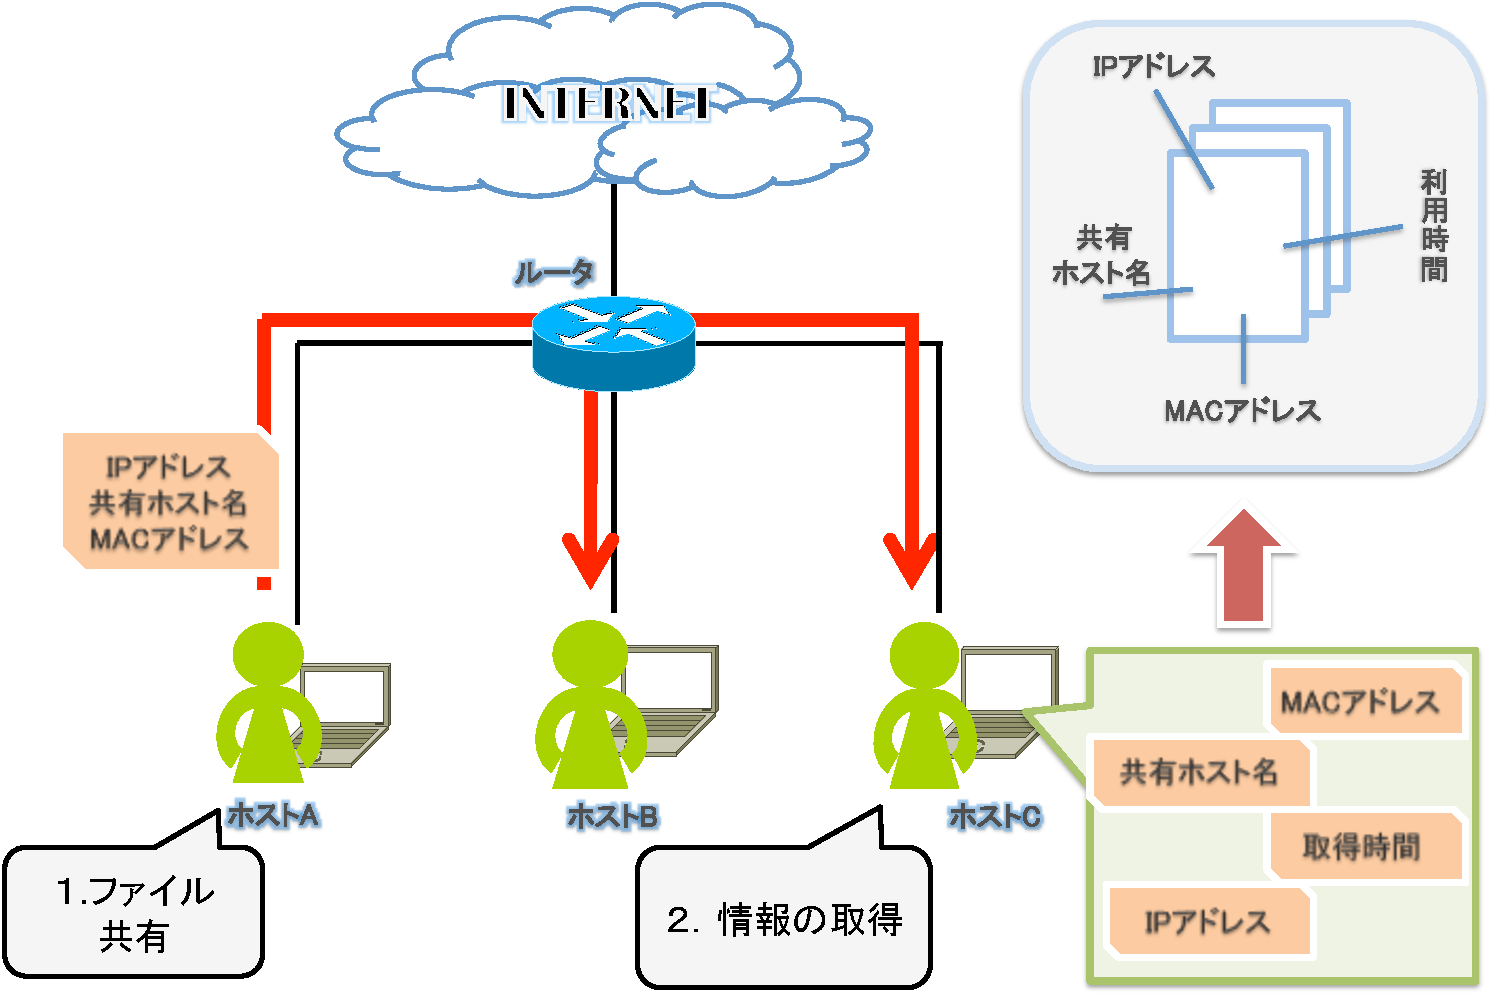
\includegraphics[scale=0.40]{./pdf/share_model}
      \caption{�ѥ��åȥإå�����μ���}
      \label{fig:share_model}
    \end{center}
\end{figure}

\subsection{��ͭ�ۥ���̾}
%1) �ʤ����ξ�������ܤ�����
�ͥåȥ������³����ȡ�OS�ˤ�äƤ�DHCP�����Ф�ץ�󥿤�Ϥ���Ȥ��뵡��
��õ�����롥õ���ϥ֥����ɥ��㥹�Ȥ�ޥ�����㥹�ȤȤ��ä��ͥåȥ��
���Τޤ���ʣ���Υۥ��Ȥ���������롥������Ǥ⡤�ե����붦ͭ�Υץ��ȥ�
��϶�ͭ�ۥ���̾��OS����Ȥ��ä��ץ饤�Х��˴ؤ�����󤬴ޤޤ�Ƥ��롥
�����ξ���ϥͥåȥ���Υȥ�ե��å������ˤ˸����뷹���ˤ��롥
���Τ��ᡤ�����ξ����������뤳�Ȥǡ��ۥ��Ȥ�桼���Υץ��ե����뤬�����Ǥ����ǽ�����⤤��

%2) �ʤ����β������Ƥ���˻�ä���
mDSN��NetBIOS�����ꤷ����ͭ�ۥ���̾�䵡��̾��ޥ�����㥹�Ȥ��������Ƥ��롥
�����ơ������ξ���ϴ�ñ�˱�����ǽ�Ǥ��롥
�㤨�С�
��\ref{fig:share_mac}�Ǥϡ�MacOSX��Finder���ץꥱ�������Υ���ץ��㡼
��ɽ�����Ƥ��롥������ɽ�����Ƥ���Τϥͥåȥ���ˤ����붦ͭ���Υۥ�
��̾��ɽ�����Ƥ��롥����ˤ�äơ����Υͥåȥ���ˤ����ơ��ɤΥۥ���
����ͭ��ǽ����Ƚ�̤Ǥ��롥�ޤ���MacOSX�ξ�硤�ǥե���ȤǶ�ͭ�����ꤵ��
�Ƥ����礬���롥���ξ�硤�桼��̾�ȥۥ��Ȥ�ɽ������롥
��\ref{fig:share_mac}�ˤ��롤{\bf ISC�Υۥ���}�����󤲤��Ƥ��뤬�����ξ��
�桼����ISC�Ȥ���̾�������ꤵ��Ƥ��롥���������ۥ��Ȥ��Ŀͽ�ͭ�Τ�Τ�
�����硤{\bf �帶ͺ����Mac Book Pro}��ɽ������Ƥ��ޤ����ۥ��Ȥν�ͭ
�Ԥ��ͥåȥ����Ǹ�������Ƥ��롥
\begin{figure}
    \begin{center}
      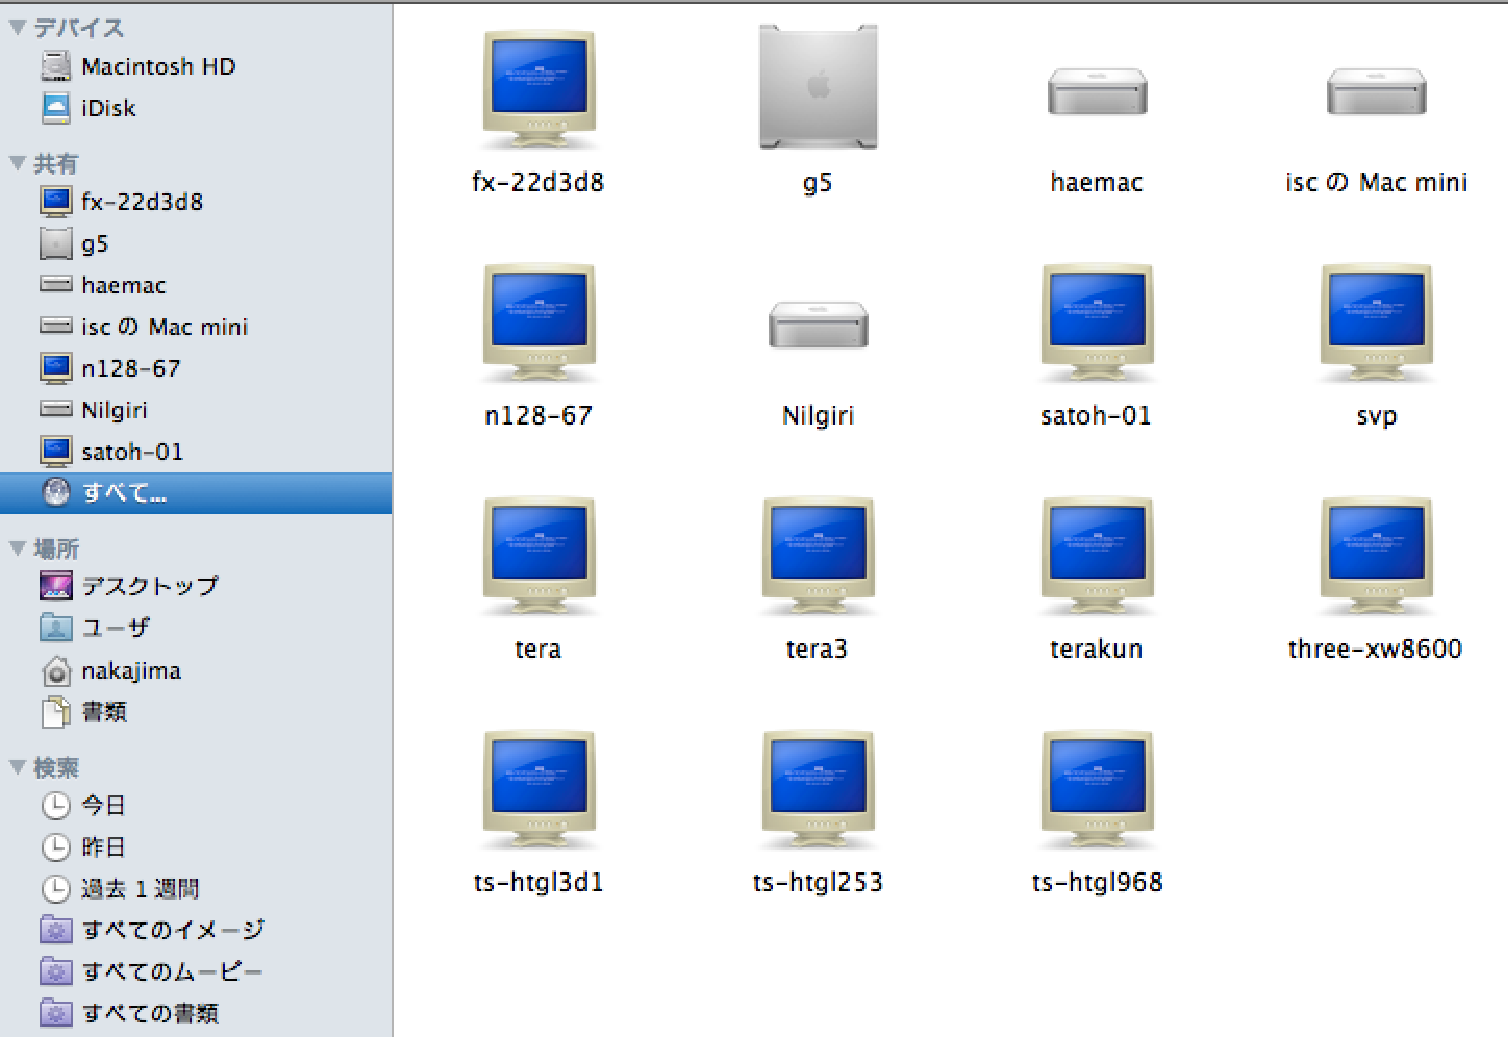
\includegraphics[scale=0.50]{./pdf/share_mac}
      \vspace{-5mm}
      \caption{MacOSX��Finder}
      \label{fig:share_mac}
    \end{center}
    \vspace{-5mm}
\end{figure}

%3) ���ξ����ɤΤ褦�����Ѥ���ȤɤΤ褦�ʷ�̤�������Τ�
��\label{fig:sharet_model}�ˤ⼨���褦�ˡ�
Ʊ�쥻�����Ȥ���³��������ǡ���ͭ����Ĥ��Ƥ���ۥ��Ȥε���̾��̾
����������뤳�Ȥ��Ǥ��롥��ͭ�ۥ���̾�����Ǥʤ��������ͭ��MAC���ɥ쥹
��Ʊ���˼����Ǥ��뤿�ᡤ�������Ȥ߹�碌�ƥۥ��Ȥ�桼�������꤬��ǽ
�Ǥ��롥�ä�MAC���ɥ쥹�Ȥ��ä���վ���ȶ�ͭ�ۥ���̾���Ȥ߹�碌��ȡ�
�ۥ��ȤȿͤΥޥåԥ󥰤��뤳�Ȥ��Ǥ��롥�����ơ����ξ�������Ѥ�������
���뤳�Ȥˤ�äơ��桼���ξ���������֤ʤɼ������Υץ��ե��������
����������Ѥ��Ƥ���ۥ��Ȥ�OS�Ȥ��ä��ץ��ե������������뤳�Ȥ�
�Ǥ��롥�ޤ�����ͤ�ʣ���Υۥ��Ȥ����Ѥ��Ƥ���桼���Ǥ��ä��ꡤ���롼
�פǶ�ͭ�����ݻ����Ƥ���ۥ��ȷ����¬���뤳�Ȥ��Ǥ��롥


%4) ���줬�ɤΤ褦�ʥ���ѥ��Ȥ�ï��Ϳ����Τ�
����ˤ�äơ��ۥ��Ȥ����ѼԤμ�����ξ����桼����������Ƥ���ۥ��ȿ���ʬ��
�롥�����ơ���ͭ�ۥ���̾��MAC���ɥ쥹���Ȥ߹�碌�뤳�Ȥˤ�äơ��ͥ�
�ȥ����ǥ桼�������פ��Ǥ���褦�ˤʤ롥

%5) �������2�Ϥ��������Ƥ��������Τɤ�ˤ�����Τ�



\section{�軰�ԤǤ���桼���ȼ�������}
%1) �ʤ����ξ�������ܤ�����
Ʊ���ͥåȥ����¸�ߤ��ʤ��桼���μ����Ǥ������ϸ��ꤵ��롥Ʊ���ͥ�
�ȥ����¸�ߤ��ʤ��桼���ϥȥ�å����оݤΥ桼�������Ѥ���褦�ʥ���
�ӥ����󶡤��뤫���桼�������Ϥˤऱ��ȯ��������������ΤߤǤ��롥

�桼�������Ϥ�ȯ���������˾��������Ƥ�ȡ�̵��LAN��Bluetooth���̿���
�󤲤��롥������ǡ��軰�ԤǤ��ưפ˼�����ǽ��Bluetooth���̿������ܤ�
����Bluetooth�ϥڥ���󥰻���Bluetooth̾����Ϥ�ȯ�����뤬�����ξ���
�桼������μ������Ǥˤʤ��ǽ�����⤤��

\subsection{����}
\label{assumption:pakcet}
Bluetooth�ξ�����������ˤ����ꡤ�������뵡���Bluetooth�����ͥåȥ
������³���뤳�ȤϤǤ���������ʳ��ξ����������뤳�ȤϤǤ��ʤ��Ȥ��롥
�ޤ�������������ΤФ�Ĥ����ɤ����ᡤ�������뵡��ϸ��ꤷ�����Bluetooth�ǥ�
������õ����³���롥


\subsection{Bluetooth}
%2) �ʤ����β������Ƥ���˻�ä���
��ǯ¿���ε����Bluetooth��Ƴ������Ƥ��롥Bluetooth�ϴ�ñ�˥桼����ȯ
�����뤳�Ȥ��Ǥ������Ϥ⤽����Τ뤳�Ȥ��Ǥ��뤿�ᡤBluetooth�ǥХ�����
�ɥ쥹���ĿͤΥץ饤�Х��˱ƶ������������Ǥ��롥Bluetooth�ϵ���ˤ��
�Ƥϥǥե���Ȥ����ꤵ��Ƥ��ꡤ�桼�����Τ餺�����Ѥ��Ƥ����ǽ��
�����롥�ޤ����桼�������򤷤����Ѥ��Ƥ�����Ǥ⡤�ץ饤�Х�����
��������ǽ�������롥�����ǡ�Bluetooth�ˤ�äƥۥ��Ȥ����Ǥʤ���������
�ʤ�Bluetooth�����Ѥ��뵡��Υץ��ե��������������ˡ���󼨤��롥

��\ref{background:user_in_network}��ǡ�Bluetooth�Υڥ���󥰤ˤĤ��ƽ�
�٤��褦�ˡ��ڥ���󥰤ˤ����ơ�������̿��ϰ����Τ�Bluetooth�ǥХ�����
�ɥ쥹���������롥���Τ��ᡤ�ͥåȥ����ǵ����ͭ�μ������ǤȤ��ư�
�����ǽ�������롥�ºݤˡ����Ӥ˥ǥե���Ȥ����ꤵ��Ƥ����礬���ꡤ
���Bluetooth�ǥХ������ɥ쥹��ȯ����³���Ƥ��륱������ͭ�롥���Τ褦
��Bluetooth�ǥХ������ɥ쥹����������ݻ����Ƥ������Ȥǥ桼���Υȥ�å�
�󥰤����ˡ���󼨤��롥�ºݤˡ��ؤʤɿͤ����ޤ�Ȥ����ǡ�Bluetooth�ǥ�
������õ�������ȥ�å��󥰤򤪤��ʤä��Ȥ�����ߤ⤵��Ƥ�
��\cite{takagi:2009}��

%3) ���ξ����ɤΤ褦�����Ѥ���ȤɤΤ褦�ʷ�̤�������Τ�
Bluetooth���ɥ쥹�ˤ�äơ�������ݻ������桼�����¬�Ǥ��롥�ޤ����ۥ��Ȥ�
�ե����붦ͭ�Ȥϰ㤤���������äʤɾ����ʵ���ޤǤ�Bluetooth���б����Ƥ�
�뤿�ᡤRFID�����Τ褦�����Ѥ�ͤ����롥����ˤ�äơ��¥桼������ư����
�����ں߻��֤ʤɤ��Ȥ߹�碌�ƥץ��ե������������뤳�Ȥ��Ǥ��롥
��\ref{fig:Bluetooth_model}�˼����褦�ˡ��ƾ����ܥ����ƥ�����֤��뤳�Ȥǡ�
���οͤ�ˬ�䤷�����֡��ں߻��֡���л��֤ʤɤ��Τ뤳�Ȥ��Ǥ��롥���Υ�
���ƥ���׽�����֤��뤳�Ȥǡ��¶��֤ˤ�����Υȥ�å��󥰤���ǽ�Ǥ��롥
\begin{figure}
    \begin{center}
      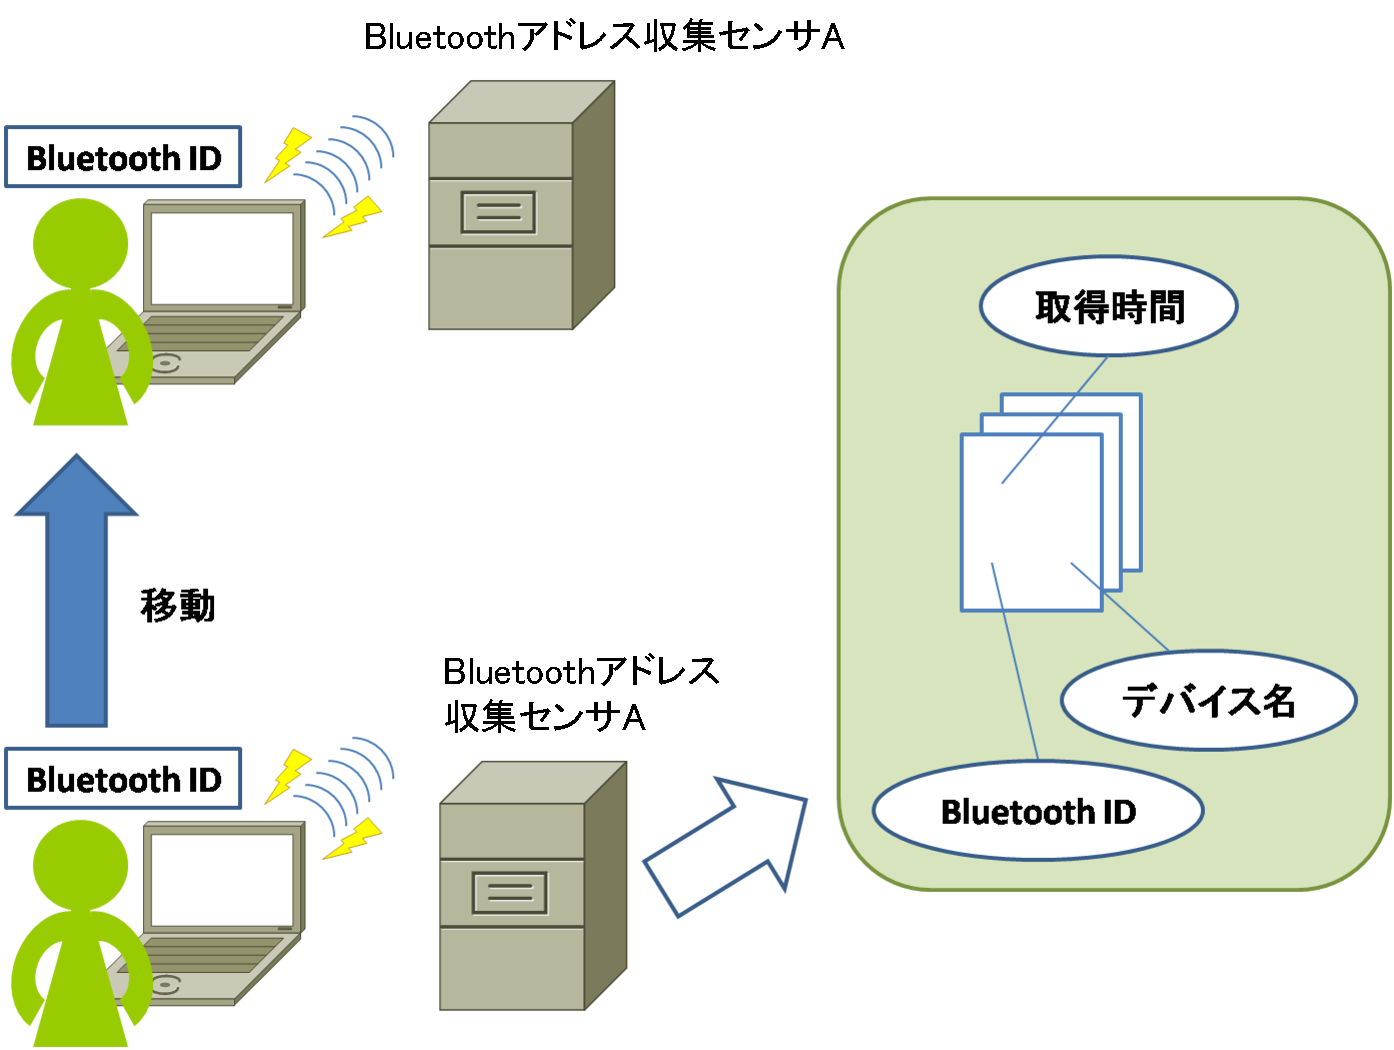
\includegraphics[scale=0.45]{./pdf/Bluetooth_model}
      \caption{Bluetooth������}
      \label{fig:Bluetooth_model}
    \end{center}
\end{figure}
%4) ���줬�ɤΤ褦�ʥ���ѥ��Ȥ�ï��Ϳ����Τ�
����ˤ�äơ�Bluetooth�����Ѥ��Ƥ��뤹�٤ƤΥ桼�����ƶ�������롥
�äˡ��¶��֤��ư������꤬��Ͽ�Ȥ����ݻ�����롥�ޤ���Bluetooth�ǥХ������ɥ쥹��
��ͭ���ѹ����Ǥ��ʤ����ᡤ���٥ץ��ե�����󥰤���Ƥ��ޤ��ȡ�
������Ѥ���ʳ������פ��ɤ����ʤ��ʤ���

�ʾ�Τ��Ȥ��餳�μ�ˡ�θ��ڤ�ɬ�פǤ��롥
Bluetooth�ǥХ������ɥ쥹����������桼���μ�����䵡���ID�����Ѥ�����
���ե�����������ɤ����٤ξ��������Ǥ���Τ��򸡾ڤ��롥

\section{���ھ�������ˤ��ꥹ��}
���ڤ����Ѥ���ѥ��åȥإå����󡤶�ͭ�ۥ���̾��Bluetooth�ǥХ���̾����
�߹�碌�뤳�Ȥǡ��ɤΤ褦�ʾ�������뤳�Ȥ��Ǥ���Τ���Ƥ���롥����
��ξ�����Ȥ߹�碌�뤳�ȤϸĿͤ����ꤹ��ˤ����궼�ҤȤʤ��ǽ������
�롥���ˡ�����Ҥ٤�������Ȥ߹�碌�뤳�Ȥ���ǽ�ˤʤ�С��ͥåȥ��
�ˤ�����Ŀͤ�ۤ����ꤹ�뤳�Ȥ��Ǥ���褦�ˤʤ롥������󡤺���󤲤�
3�Ĥξ�������ǤϤʤ��������ξ�����������ˤ����ꡤ���Ѥ�������
�٤Ƥ����Ѥ��뤳�Ȥǥۥ��Ȥ����Ѥ���桼����ľ������Ǥ��롥


\section{�ޤȤ�}
�ܾϤǤϡ��桼���Υץ饤�Х��򶼤��������ˤĤ���3�Ĥμ�ˡ���󼨤�����
�ޤ����ѥ��åȤΥإå�����������Ȥ˥桼���Υץ��ե��������������ˡ��
�ե����붦ͭ����mDNS�ץ��ȥ�������Ѥ���붦ͭ�ۥ���
̾��NetBIOS��NetBIOS̾�����Ѥ��ơ��ۥ������ѼԤ�����������Υꥺ���
���־������������ˡ��Bluetoothõ���ˤ�����ǥХ������ɥ쥹��̾������
�Ѥ������פ����ˡ��3�ĤǤ��롥��\ref{evaluation}�ϤǤϤ����μ�ˡ���
�ݤ˸��ڤ��롥



%%% Local Variables:
%%% mode: japanese-latex
%%% TeX-master: "../nakajima_bthesis"
%%% End:

\chapter{����}
\label{evaluation}
�ܾϤǤϡ���\ref{assumption}�ϤǽҤ٤��桼�������ˡ�򤽤줾�측�ڤ��롥
�ޤ������ڤ����Ѥ�����������礹�뤳�Ȥˤ�붼�ҤˤĤ��ƽҤ٤롥
\section{�ѥ��åȤΥإå�����}
�ѥ��åȤΥإå���������Ѥ��뤳�ȤǤɤ��ޤǥۥ��Ȥ��̲�ǽ�ʤΤ���
�ڤ��롥�����������ϼ��5���ץ�ȸƤФ�롤�����衦������IP���ɥ쥹��
�����衦�������ݡ����ֹ桤�ץ��ȥ���Ǥ��롥
\label{evaluation:pakect}
\subsection{���ڼ�ˡ}
\label{evaluation:packet:meth}
�ͥåȥ���ˤ����ƥۥ��Ȥ����Τ˼��̲�ǽ���θ��ڤ�Ԥ���������
�������åȥ桼����Ʊ�դ�����MAC���ɥ쥹��������롥�ۥ��ȼ��̤ˤ����ꡤ
MAC���ɥ쥹����Ѥ��ʤ��������������ڻ��˥ۥ��ȼ��̤�����Ƚ������Ѥ��롥
�ޤ����������åȥۥ��ȤΥץ��ե���������ۥ������ѼԤ��󵭤��뤳�Ȥǡ�
���ڤ��롥

���ڼ�ˡ��ɾ���ϡ��ۥ��Ȥ�ʬ�ࡦ���̤����٤Ȥ��롥�����ơ��ɤΤ褦�ʾ�
�ﲼ�ǥۥ��ȼ��̤���ǽ�ʤΤ����⤷���ϼ����˼��Ԥ���������������롥��
���Ǥϡ��ۥ��Ȥ��Ф���ץ��ե����������Ԥ������Υץ��ե����뤷����
��ȹ��פ�����硤Ʊ���ۥ��ȤǤ����Ƚ�Ǥ��롥

\subsection{�ۥ��ȼ��̥����ƥ�}
�ͥåȥ���Υȥ�ե��å�����ƥ桼��������������ѥ��åȾ������³
���֤����ѻ��֤ʤɾ����ʬ�Ϥ��뤳�Ȥǡ��ۥ��Ȥ��̤��롥�ۥ��Ȥ˴ؤ�
�����ϡ��ͥåȥ��������������ܸ�����Ѥ����ȥ�ե��å��ƻ����֤�
���֤��뤳�Ȥǡ����Ū�˼������롥���Τ��ᡤ�ܥ����ƥ�����ѼԤ��оݥͥ�
�ȥ�����̿���ƻ뤹�븢����ͭ�ԡ��⤷���ϥͥåȥ�������Ԥ������
���줿�桼���Ǥ��롥

\begin{figure}
    \begin{center}
      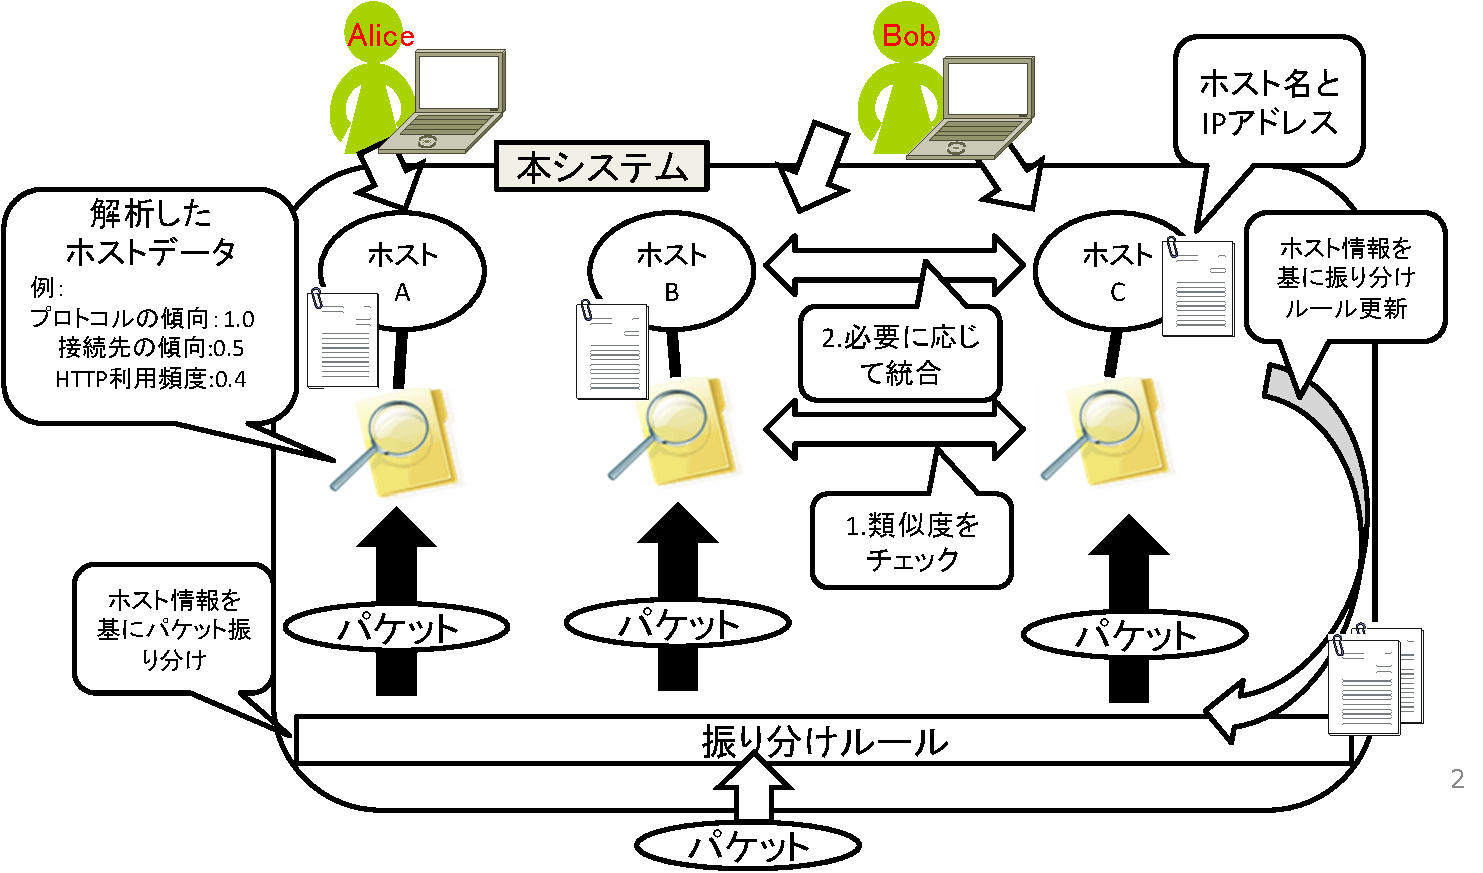
\includegraphics[scale=0.65]{./pdf/system_model}
      \caption{�����ƥ��ư���}
      \label{fig:user_model}
    \end{center}
\end{figure}

�����ƥ��ư��פ��\ref{fig:user_model}�˼������桼����Alice�ϡ��ܥ�
���ƥ�ˤ����ƥۥ���A�Ȥ��ƿ��ꤵ��ơ������롥�����ǡ��ۥ���A�����
¬�Ǥ����������Ѥ��ƥץ��ե������������롥���Υץ��ե����������
�Ȥˡ��ۥ��Ȥϥȥ�ե��å�������־����ۥ��Ⱦ���ʤɤξ�����������
�ǡ����١����˳�Ǽ���롥���������ۥ��ȼ��̤����Ѥ������ϡ��ۥ��Ȥ���
ħ��դ�ޤ������������뤿�ᡤBob�Τ褦��ʣ���ˤޤ�����ۥ��Ȥ����ꤹ
�롥���ξ��ϡ����Ū�˥ۥ��ȴ�Ʊ�ΤǶ��̻����õ������ȯ���������
�ϳ�������ۥ��Ⱦ�������礹�롥

\subsection{�߷׳���}
�ܥ����ƥ�ϥͥåȥ������������˥ȥ�ե��å��ƻ����֤����֤���
���Ū�˥ѥ��åȤΥإå������������뤳�Ȥǡ��ۥ��Ȥ��̤��롥
�ۥ��Ȥ��̤����ܥ����ƥ�ϡ��礭��2�Ĥ�ư���ʬ�����롥
IP���ɥ쥹����ۥ��Ȥ�Ƚ�ꤹ��{\bf IPȽ��⥸�塼��}���ۥ��Ⱦ�Υ��ץꥱ��������ư���ۥ��Ȥ�ʬ�ह��
{\bf ���ϥ⥸�塼��}�Ǥ��롥�ۥ��ȼ��̼�ˡ���߷פ��\ref{fig:tree}�˵�����

\begin{enumerate}
\item{{\bf IP���ɥ쥹Ƚ��⥸�塼��}}\\
  ��IP���ɥ쥹Ƚ��⥸�塼��ϡ��ѥ��åȤ�IP���ɥ쥹���ˡ��ۥ��Ȥ��
  �ꤹ�롥�ͥåȥ����DHCP�꡼�������������˳�������IP���ɥ쥹�Ϥ�
  �٤�Ʊ���ۥ��ȤǤ����Ƚ�Ǥ��롥��������DHCP�꡼�������������˳���
  ����IP���ɥ쥹�����̿����ʤ��ä����ϡ����Υۥ��Ȥϥͥåȥ������
  Υ�줿��ΤȤ��롥
\item{{\bf �ѥ�������ϥ⥸�塼��}}\\
  ���ۥ��Ⱦ�Υ��ץꥱ��������ư���ۥ��Ȥ�ʬ�ह�롥���Υ⥸�塼
  ��Ͼ����˱�����ʣ���ĺ������롥�ޤ��ƥ⥸�塼�뤴�Ȥ˥ѥ���������
  ���륢�르�ꥺ����Ѳ����롥�㤨�С��᡼�륵���Ф˥��������������٤�
  �����桼����ʬ�ह�뤿��μ������ǤȤ��롥
\end{enumerate} 

�ƥ⥸�塼����������ۥ��Ȥ�ȯ��������硤�ۥ��Ȥ���ͭ��������
��������ۥ��Ȥξ�������礵��롥�����ơ������Υ⥸�塼��ˤ��
�ƿ����ۥ��Ȥ���¸�Υۥ��Ⱦ���ȥޥå����ʤ��ä����ˤϤ���ơ�������
�ۥ��Ȥ���������롥���������κ�Ȥ򷫤��֤��뤳�Ȥˤ�äơ��ۥ��Ȥ��̤��롥

\begin{figure}
    \begin{center}
      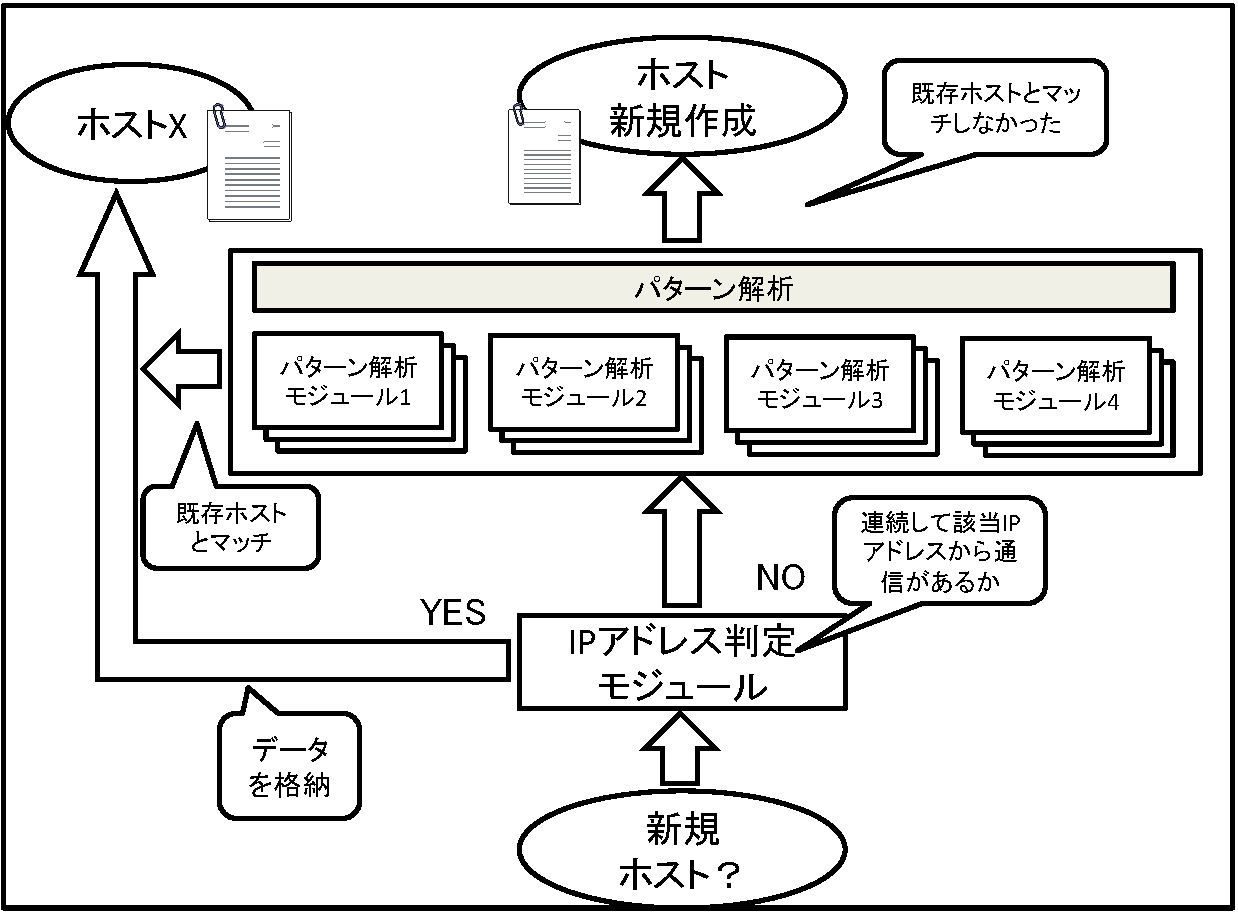
\includegraphics[scale=0.65]{./pdf/tree}
%      \vspace{-5mm}
      \caption{�ۥ��ȼ��̼�ˡ���߷�}
      \label{fig:tree}
    \end{center}
\end{figure}

�ܥ����ƥ���׷���Ф��뽼­�٤ˤĤ��ƽҤ٤롥�ܥ����ƥ�ϡ��ͥ�
�ȥ����������������֤�������ǥۥ��ȼ��̤���ǽ�ˤʤ뤿�ᡤ�����Ԥ�
��뱿�Ѥ��ưפǤ��롥���ˡ��ۥ��ȼ��̤����٤˴ؤ��Ƥϡ��ܿͤȿ�¬�Ǥ�
������¿���Ȥ߹�碌�뤳�Ȥˤ�ä����٤θ����ޤ롥�����ơ����Ū�˾�
�����������ꥢ�륿����˥ۥ��Ȥ��̤򤹤뤳�Ȥ��Ǥ��롥�ޤ���
�ܥ����ƥ���絬�ϥͥåȥ���ξ�ή�����Ѥ��뤿�ᡤ�ͥåȥ���夹�٤Ƥ�
�ۥ��Ȥ��оݤȤ��뤳�Ȥ��顤�桼�����������Ϥ���ȸ����롥�ޤ����⥸�塼
����ɲä��ưפǤ��롥


\subsection{�ۥ��ȼ��̤��Ѥ������}
\label{sec:���̾���} 
�ۥ��Ȥμ��̤��Ѥ������ϡ��ۥ��Ȥ����Ǥ������Ǥ��롥
��������Ѥ���������\ref{assumption:used}��ǽҤ٤��ʲ��ξ�������Ѥ��롥

\begin{itemize}
\item{\bf ������IP���ɥ쥹�ȥݡ����ֹ���Ȥ߹�碌}\\
  ��������IP���ɥ쥹�ȥݡ����ֹ���Ȥ߹�碌��Ĵ�����롥���Ѥ���ץ���
  �����SSH��IMAP,VPN,IRC�˸��ꤹ�롥���Υץ��ȥ����3��ʾ�Ʊ���ۥ���
  ���Ф����̿����Ԥ�줿��硤�������ǤȤ��ƥꥹ�Ȥ˲ä��롥

\item{\bf ȯ�����ݡ����ֹ�}\\
  ���ۥ��Ȥ�ȯ�����ݡ����ֹ椫��OS�����ꤹ�뼱�̤Ȥ��롥���Ҥ����褦��
  ���Ѥ��Ƥ����������ݡ����ֹ椫��OS�μ���򤪤��ޤ��ǤϤ��뤬ʬ�ह��
  ���Ȥ��Ǥ��롥IP���ɥ쥹����Ϳ�����1ʬ�֡��оݥۥ��Ȥ�ȯ�����ݡ���
  �ֹ��Ͽ���롥���ˡ�ȯ�����ݡ��Ȥ�1024-5000����49152-65535�ɤ����
  �ϰϤ˶ᤤ����Ƚ�ꤷ���������Ǥΰ����Ȥ��롥�ޤ����ۥ��Ȥ��ٻ߾��֤���
  ���줷����硤Ϣ³�����ݡ����ֹ�����Ѥ��뤿�ᡤ�ۥ�����˺Ǹ�����Ѥ����ݡ���
  �ֹ�򵭲����롥
\item{\bf �ѥ��åȤ�ȯ�������ߥ�}\\
  ���ѥ��åȤ�ȯ�������ߥ󥰤ˤ�äơ�OS��������뤳�Ȥ��Ǥ��롥�ۥ���
  ��ư����IP���ɥ쥹����Ϳ����Ƥ���2ʬ�ּ��������ޥ�����㥹�Ȥ����
  ��TCP���̿����ǽ��ȯ�����륿���ߥ󥰤��¬���롥Windows�ξ��, IP��
  �ɥ쥹����Ϳ����Ƥ���30�����TCP�ˤ��Update��ǧ���̿���ȯ�����뤳��
  ����ǧ����Ƥ��뤿�ᡤȽ�̤���ǽ�Ǥ��롥�ޤ���IP���ɥ쥹����Ϳ�����
  ����5�ð���˿�����TCP�ѥ��åȤ�ȯ�����줿��硤���Υۥ��Ȥϡ��ٻ߾�
  �֤�������졤�⤷���Ϥ��Ÿ��򤤤줿�ޤޥͥåȥ�����ư������Ƚ��
  ���롥
\item{\bf ���ѥ��ץꥱ������󡤥����ӥ�}\\
  �������ӥ����󶡤��륵���ФΥ��ɥ쥹�֥��å����Ѱդ����ۥ��Ȥ��̿���
  �������ФȾȤ餷��碌�뤳�Ȥǥۥ��Ȥ����Ѥ��Ƥ��륢�ץꥱ��������
  �����ӥ������ꤹ�롥�ޤ������եȥ����������Ǥʤ�OS��Update���̿�����
  �ݤȤ��롥

\end{itemize} 

\subsection{���ڴĶ�}
\label{evaluation:packet:env}
2009ǯ9��7���ʷ�ˤ���10�����ڡˤˤ����ơ�Ĺ�Ĺ��Ծ���Į�ˤƳ��Ť�
�줿WIDE��ɤˤ�����ͥåȥ���Ǽ¸���Ԥä���
��ɥͥåȥ���Ϥ�200��ʾ�Υۥ��Ȥ����ä��Ƥ��ꡤ��°���륳�ߥ�˥ƥ����͡�
�Ǥ��롥
����WIDE��ɥͥåȥ���ȥݥ����ޤ��\ref{fig:wide_net}�˼�����
\begin{figure}
    \begin{center}
      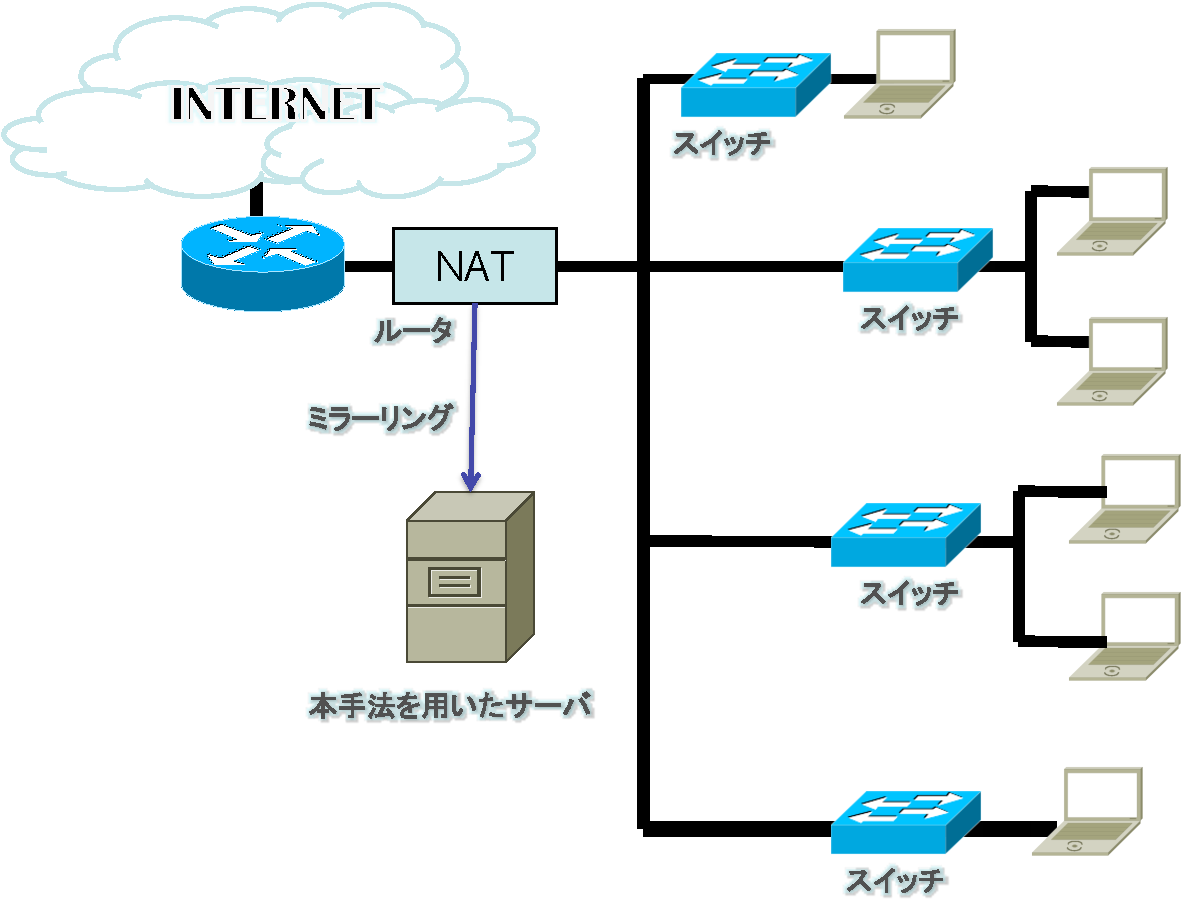
\includegraphics[scale=0.50]{./pdf/wide_top}
      \caption{WIDE��ɥͥåȥ���ȥݥ�����}
      \label{fig:wide_net}
    \end{center}
\end{figure}
���Υͥåȥ���Ǥ��٤Ƥ�̵�������Ѥ����ۥ��ȤΥѥ��åȥإå���
������Ѥ��ƥۥ��Ȥμ��̤�Ԥ���
��ɤǥѥ��åȤ�����������֤�2009ǯ9��7��17��44ʬ����9��9��16��8ʬ�ޤǤǤ��롥

%�⤦�ҤȤĤδĶ��ϡ�ɮ�Ԥν�°���븦�漼��Ʊ�����롼�פΥ��С�����̾
%�ε��Ĥ����ơ��ѥ��åȾ����������롥���漼�Υͥåȥ���ΰ���������
%���ơ�����Υ����å������Ѥ������ˡ��ȥ�ե��å����������褦�ˤ��롥
%��\ref{fig:nakajima_net}�˼¸��ѥͥåȥ���Υȥݥ����򵭤���
%
%\begin{figure}
%    \begin{center}
%      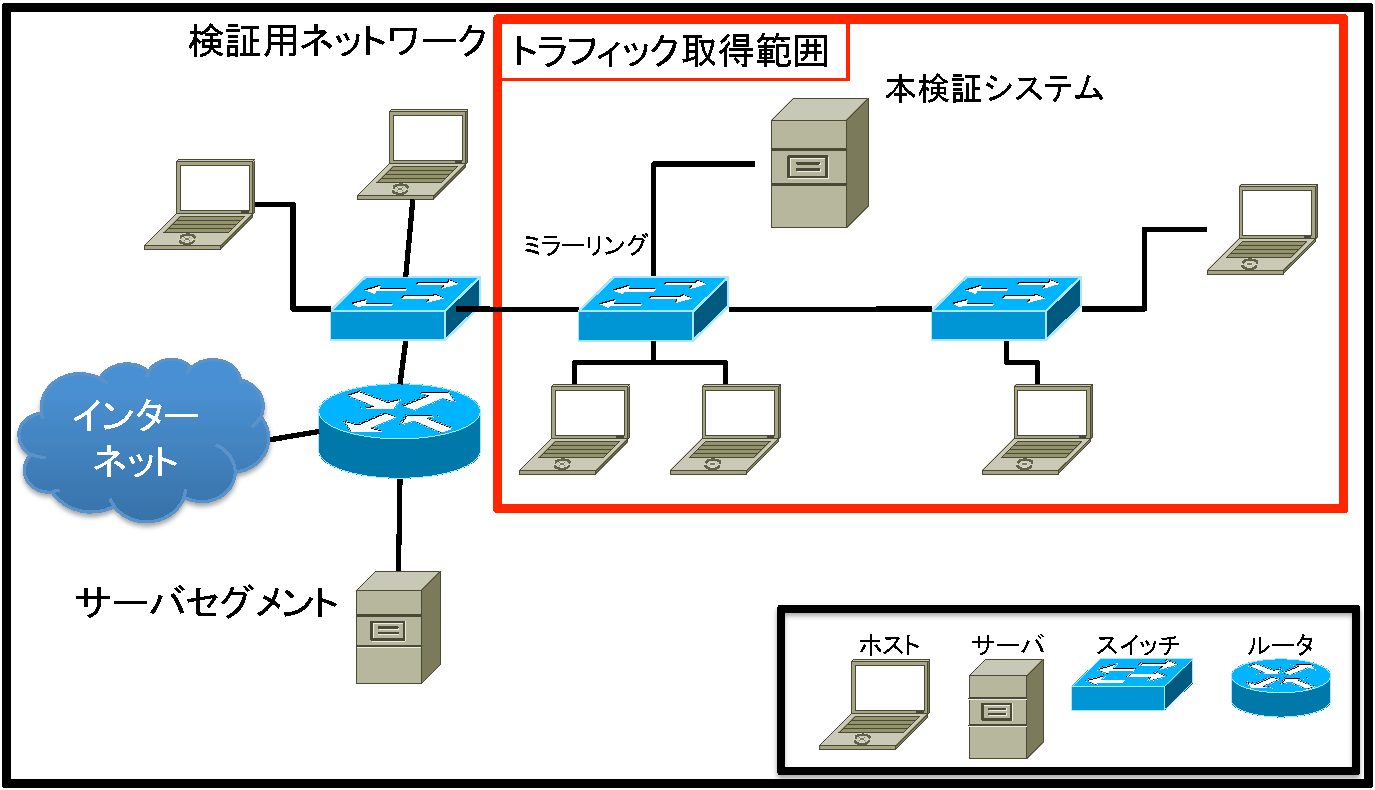
\includegraphics[scale=0.50]{./pdf/nakajima_network}
%      \caption{���漼���ѥͥåȥ�����׿�}
%      \label{fig:nakajima_net}
%    \end{center}
%\end{figure}
%
%���Ҥ���WIDE��ɥͥåȥ���Ȥΰ㤤�ϡ�Ʊ�����ߥ�˥ƥ��˽�°����桼
%���Υۥ��Ȥ����ѤǤ��뤫����Ū�Ȥ��Ƥ��롥
%

\subsection{���ڷ��}
\label{evaluation:packet:res}
%\begin{itemize}
%\item{\bf WIDE��ɥͥåȥ��}\\

\begin{table}
\caption{WIDE��ɥͥåȥ���ˤ�����¸����}
\label{tb:head_result}
\begin{center}
{\footnotesize
\begin{tabular}{|*{7}{l|}}
%1mail 2keio 3google,4other
%1cpu kccx 3other
\hline
�������ǡ��ۥ���&$H_1$&$H_2$&$H_3$&$H_4$&$H_5$&$H_6$\\
\hline
Mail Server   &$S_1$,$S_2$&$S_1$,$S_2$&$S_6$&$S_1$,$S_2$&$S_2$&$S_1$,$S_2$\\
              &$S_3$&$S_4$,$S_5$&  &  &  &  \\
\hline
SSH Server    &$S_1$,$S_3$&$S_1$,$S_6$&$S_1$&&&\\
              &$S_4$,$S_5$&$S_7$,$S_8$&  &  &  &  \\
              &     &$S_9$&  &  &  &  \\
\hline
�ѥ��åȴֳ֤���  &MacOS&MacOS&Windows&MacOS&Windows&MacOS\\
��¬�����OS  &&&&&&\\
\hline
�������ݡ���&49152-65535&49152-65535&1024-5000&49152-65535&49152-65535&49152-65535\\
\hline
IRC Server&&&$S_1$,$S_2$&&&\\
          &&&$S_3$,$S_4$&&&\\
\hline
��ħŪ�ʵ�ư&���Ū��&&&&�ü��&VPN��\\
        &HTTP�̿�&&&&ȯ����&���Ū��\\
        &��������&&&&�ݡ�������  &HTTP�̿�\\
\hline
MSN�Υꥹ����&5383&1972&8862&13166&&1362\\
\hline
��ư���ε�ư&HTTP�̿�&&HTTP�̿�&MSN&        HTTP�̿�&\\
            &IMAP��³&&        &��å��󥸥�&&\\
\hline
Update&Evernote&MacOS&Windows&MacOS&Firefox&MacOS\\
      &MacOS   &     &       &     &Quick Time&Safari\\
\hline

\end{tabular}
}
\end{center}
{\bf H}:�ۥ��� {\bf S}:������\\
\end{table}

\subsubsection{�ۥ��Ȥ�ʬ��}
WIDE��ɤˤ�����ͥåȥ������6��Υۥ��Ȥ�ʬ��Ǥ��뤫�Ȥ������ڤ�
�����ơ��������Ǥˤ���ˡ���Ѥ�����ɽ\ref{tb:head_result}�ˡ�
�¸���̤򼨤���

�ޤ���SSH��IMAP�ˤ����밸��ۥ��Ȥ�ʬ�ष���������
���ߥ�˥ƥ��˽�°���Ƥ���桼����Ʊ�������Ф����Ѥ��뷹���ˤ��뤿�ᡤ
����ۥ��Ȥ��������������ưפ�ʬ�ब��ǽ�Ǥ��롥����ˤ�äơ�200��ʾ��
�ۥ��Ȥ���13��ޤǹʤ뤳�Ȥ��Ǥ��롥���ˡ�SSH��IMAP���ѼԤˤ����ƥȥ�ե���
�������̤������ǤȤ�����硤12��Υ桼������ħ�դ���Ԥä���SSH��IMAP��
��³���12��Υ桼���ϳơ���ʬ�����롥

IMAP����³��˾��������Ƥ�ȡ��礭��3���Mail�����Ф����Ѥ���Ƥ��뤳��
��ʬ���롥���˾ܤ������Ϥ���ȡ�$H_1$,$H_2��$¿���Υ᡼�륵���ФȤ���
�ꤹ�뷹��������Τ��Ф��ơ�$H_3$��ʣ���Υ�������Ȥ����᡼�륵���Ф�
���礷�Ƥ����ǽ�����⤤�������ơ�SSH����³��򸫤�ȡ�$H_1$,$H_2$��ʣ
���Υۥ��Ȥ����Ѥ��Ƥ��롥SSH��IMAP�����Ѥ�������dzƥ桼����ʬ��ϲ�ǽ��
���롥

���ˡ���å��󥸥��IRC�����Ѥ��Ƥ���桼����ʬ�ष������å��󥸥����
�Ѥ����硤�̿���Ԥ����Υꥹ�Ȥ����ꤹ�롥���Υꥹ�ȤΥȥ�ե���
����(byte)��桼�����Ȥ�ʬ��������å��󥸥�Υ桼���ꥹ�Ȥ��������뤿
�ᡤ100byte���٤�������äƤ��롥����ˤ�äơ�MSN��å��󥸥�����Ѥ�
�Ƥ���桼�����٤Ƥ���ħ����Ф��뤳�Ȥ��Ǥ������ޤ����ͥåȥ�����
�δط��塤�ۥ��Ȥ򥵥��ڥ�ɤ򤹤�桼����¿���������ᡤ������λ��֤�
�������ݡ��Ȥ����Ѥ��뤳�Ȥˤ�äơ���³���ƥ桼����ȥ�å��󥰤��뤳
�Ȥ��Ǥ�����

��ư���Υѥ��åȤȥ������ݡ����ֹ���¬���뤳�Ȥˤ�ä�5�椬MacOS�Ǥ�
�ꡤ2�椬Windows�Ǥ��뤳�Ȥ�ʬ���ä��������ơ��ͥåȥ����³����OS��
���եȥ�������Update���ǧ���Ƥ��뤫�ƻ뤷�������κ�
�ˡ�FireFox�����Ѥ��Ƥ���桼����4̾ȯ������Ƥ��롥
�ޤ������ץꥱ����������ѻ���ȯ������ȥ�ե��å���
�顤Evernote\cite{evernote:2010}�ʤɤ�ư�������ꤷ�Ƥ���ۥ��Ȥ�Ƚ��
���Ƥ��롥

��ħŪ���̿��ˤĤ��ƽҤ٤롥$H_1$�ϵ�ư�����������֤��Ȥ�Ʊ�������Ф�
�Ф���HTTP�ǥǡ������������뷹�������롥���Τ��Ȥ��顤���餫�Υ��ץ�
��������󤬵�ư���Ƥ��뤳�Ȥ��狼�롥����ϡ����ץꥱ����������ѻ�����
�������ФΥ��ɥ쥹�֥��å����ݻ����Ƥ���Ȳ��ꤷ�Ƥ��뤿�ᡤ���Υ��ץ�
���������Evernote�Ǥ����Ƚ�����Ƥ��롥Ʊ����$H_6$�ⵯư������Ʊ������
�Ф˥���������³���Ƥ��뤿�ᡤ���󥢥ץ��ư��ư�����ꤷ�Ƥ���ȸ���
�롥$H_5$�Ǥ�ȯ�����ݡ����ֹ�η�����49125-65535�֤����Ѥ���OS�Ǥ��뤬��
ȯ�����ݡ����ֹ�1444���٤�Ϣ³���ƾ�����Ѥ��Ƥ��롥���Τ��ᡤ�ü��
�����ӥ������Ѥ��Ƥ���ȿ�¬�Ǥ��롥�ޤ�����ư�������HTTP�����Ѥ�����
��������ɤ��Ƥ���Τ���¬���줿��$H_5$�ϵ�ư���Υѥ��åȤΥ����ߥ󥰤�
��Windows�Ǥ��뤳�Ȥ�Ƚ�����Ƥ��뤿�ᡤ����������륹���եȤΥ����ͥ���
�ι����Ǥ����ǽ�����⤤���ºݤ��̿���IP���ɥ쥹����Avast�ȸƤФ�륢��
�������륹���եȤ����Ѥ��Ƥ����Ƚ�Ǥ��줿��$H_6$�Ǥϡ�VPN�����Ѥ����
�Ȥ�˵�ư���������Ū��HTTP�̿��򤷤Ƥ��롥����鼱�����Ǥ��Ȥ˥ۥ�
�Ȥ�ʬ�ह�뤳�Ȥǡ��ۥ��Ȥ��Ȥ���ħ��ʬ����ɽ�����Ȥ��Ǥ��롥������
�������Ǥ�ʬ�ष�����6����6�椹�٤Ƥ��դ�ʬ�ह�뤳�Ȥ��Ǥ�����

\subsubsection{�ۥ��Ȥμ���}
�ۥ��Ȥ�ʬ�ह�뤳�Ȥ������������Ǥ����Ѥ��ơ��ۥ��ȼ��̤��롥���̤�ɬ
�פʾ����Mail �����Ф⤷����SSH �����ФؤΥ��������Ǥ��롥����ˤ��
�ơ�200��ʾ夢��ۥ��ȷ�����10��������������뤿�ᡤ������³��ȥݡ�
���ֹ�Υ��åȤ��Բķ�Ǥ��롥���μ������Ǥȹ����̤ξ����ä��뤳�Ȥ�
���ƥۥ��Ȥ���̤˼��̤Ǥ��롥�ݡ����ֹ����³����Ȥ߹�碌�ʳ���
�ϡ�MSN��å��󥸥�Υȥ�ե��å��̤�ͭ�ѤǤ��롥����ϡ���å��󥸥��
��硤Ϣ����Υꥹ�Ȥο��ϥ桼�����Ȥ˰ۤʤ��ǽ�����⤤���ᡤ�ۥ��ȼ�
�̤����Ѥ��䤹�����ޤ�����ư���ε�ư���顤����Υۥ��Ȥ˥��������򤹤�
����ˡ����ѥ��ץꥱ�����������ǤȤ��뤳�ȤǼ��̤Ǥ��롥

%\item{\bf ���漼�¸��ͥåȥ��}\\
%ɾ���桪��


%\end{itemize}

\subsection{�ͻ�}
����ۥ��ȡ��ץ��ȥ��롤���ѥ��ץꥱ������󡤵�ư���ε�ư���ѥ��åȤ�
�����ߥ󥰤��Ȥˡ����٤ƤΥ桼�����̤��뤳�Ȥ��Ǥ�����IMAP��MSNMS�Υ�
��ե��å��̤���ۥ��Ȥ��̤����ˡ��ͭ���Ǥ��롥�ޤ��������ڥ�ɤ���
����������פ��뤿����������ݡ��Ȥ����Ѥ����ˡ��ͭ���Ǥ��뤳�Ȥ�����
���������ơ���³Ū�˥ۥ������פ��뤳�Ȥǡ����ץꥱ�������Υ��åץǡ�
�Ȥ��ͭ���̿������뤳�Ȥǡ��ۥ��ȤΥץ��ե�����������Ǥ��롥���Τ褦
���͡��ʾ�����Ȥ߹�碌�뤳�Ȥǡ��ѥ��åȤΥإå���������Ǥ�ۥ��Ȥ�
���̤ϲ�ǽ�Ǥ��롥

��������IMAP��MSN��å��󥸥�Υץ��ȥ���ϡ��桼�����������٤�HTTP����
�������Ѥ����ʤɡ��桼���ο����񤤤��礭���Ѳ����Ƥ����ޤ����ᡤ����
���ǤȤ��Ƥʤ��񤤡��ޤ��������ӥ������ꤹ�뤿��ˡ������ӥ����륢�ɥ�
���֥��å����ݻ����Ƥ��뤬�����ɥ쥹�ϰϤ������ʾ�硤�ܥ����ƥ�μ���
���ǤȤ������Ѥ��Ƥ�����󤬼��ʤ���礬���뤳�Ȥ�ʬ���ä������塤��
�٤򤢤��뤿��ˡ����¿���μ������Ǥ��ɲä���ɬ�פ����롥


%%% Local Variables:
%%% mode: japanese-latex
%%% TeX-master: "../nakajima_bthesis"
%%% End:

%%%%%%%%%%%\chapter{����}port2 
%%%%%%%%%%%%%%%%%%%%%%%%%%%%%%%%%
\section{��ͭ�ۥ���̾}
\label{evaluation:share_host}
Ʊ���ͥåȥ���ˤ�����桼������ͭ�ۥ���̾�������������ǥ桼���Υ�
���Ȥ˴ؤ�����󤬼����Ǥ��뤫�򸡾ڤ��롥������������SMB��mDNS�ץ�
�ȥ���Ǥ��롤��ͭ�ۥ���̾��MAC���ɥ쥹�Ǥ��롥�����ξ�����Ѥ��ơ��桼
���μ������ۥ��Ȥ�OS���󡤥ۥ��Ȥν�ͭ�Ԥ��¬���롥

\subsection{���ڼ�ˡ}
\label{evaluation:share_host:met}
���ڼ�ˡ�Ȥ��Ƥ�ɮ�Ԥ���°���븦�漼�Υͥåȥ�����ܸ��ڼ�ˡ���Ѥ����ۥ��Ȥ���³����
����������³���롥�����������֤�2009ǯ11��18������20������3���֤Ǥ��롥
���������ۥ���̾���Ȥˡ��桼���Υۥ��Ⱦ���������Ǥξ�����ӤĤ��롥
�����ơ��ۥ���̾��MAC���ɥ쥹���ӤĤ��ơ��ꥹ�Ȳ�������¸���롥

\subsection{�߷׳���}

\begin{table}
\begin{center}
\caption{��ͭ�ۥ���̾�μ�ˡ���ڤμ����Ķ�}
  \vspace{5mm}

\label{tb:share_name}
\begin{tabular}{|c|c|c|c|}
\hline
���͸���&version&�饤�֥��&OS\\
\hline
C����&4.2.1&libpcap&FreeBSD7.2\\
\hline
PHP&5.3&&MacOSX 10.6.2\\
\hline
\end{tabular}
\end{center}
\end{table}

���ڤ�Ԥ��ץ�������ɽ\ref{tb:share_name}�ǵ󤲤�褦��libpcap�ˤ��
�ѥ��åȥ���ץ����C����ǵ��Ҥ��롥�ץ��ȥ���̾�ȥݡ����ֹ�
��NetBIOS��mDNS��Ƚ�̤����ڥ������ɤ���ۥ���̾�Τߤ���Ф�
�롥NetBIOS�ϼ��Ȥζ�ͭ�ۥ���̾����ȯ�����ʤ�����mDNS�ξ��ϥۥ��Ȥ�����
�Ƥ��붦ͭ�ۥ���̾�Υꥹ�Ȥ��������뤿�ᡤ�ޤȤ�Ƽ������롥SMB�ξ���
��ͭ�ۥ���̾��MAC���ɥ쥹�η�ӤĤ����ưפǤ��뤬��mDNS�ˤ��ꥹ�Ȥ���
��ͭ�ե�����̾������������ϡ�MAC���ɥ쥹�Ȥη�ӤĤ����񤷤��������ǡ�
�ꥹ�Ȥ��鶦ͭ�ե�����̾������������ϡ��ꥹ�Ȥ˵��ܤ��줿��ͭ�ե���
��̾�Υۥ��Ȥ��̿�����ޤǥȥ�ե��å���ƻ뤷��MAC���ɥ쥹�������Ǥ���
�褦�ˤʤ�С�������Ȥ߹�碌���ˡ����Ѥ��롥�����ơ������Ȥ߹�碌��
�������¸���롥
%�֤����ۥ���̾��MAC���ɥ쥹�Τɤ��餫�����פ����ȥ�ե��å���������롥

�ȥ�ե��å�������������塤FreeBSD��ǽ�������
���Ϸ�̤�PHP�ǵ��Ҥ���������ץȤˤ�äơ�����ղ�������

\subsection{���ڴĶ�}
\label{evaluation:share_host:env}
�����ϰϤϥ����å��ˤ��������¤�����ʤ����ᡤ���漼���̤Υͥåȥ���������������ǽ�Ǥ��롥
�����ǡ����漼�Υͥåȥ���ˤ����ơ�2009ǯ10��18������21���ޤ��ܥ����ƥ�μ¸���Ԥä���
��\ref{fig:share_topo}�˶�ͭ�ۥ���̾���Ѥ����¸��Υͥåȥ�����׿ޤ򼨤���
\begin{figure}
    \begin{center}
      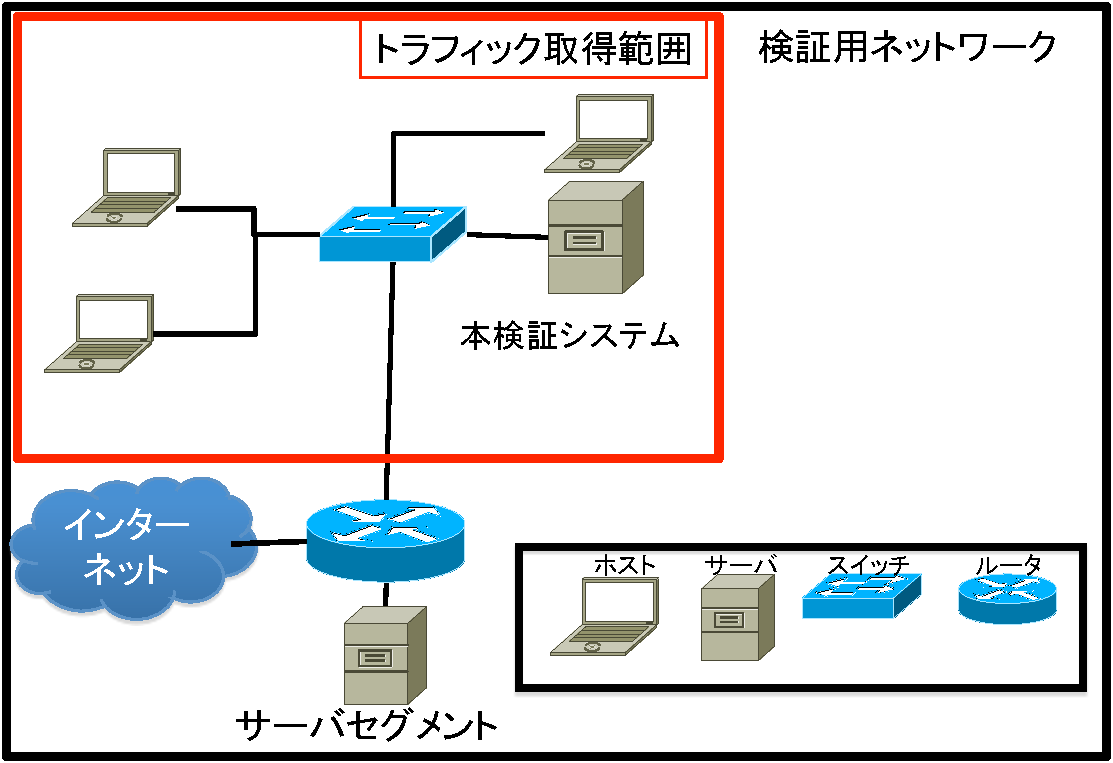
\includegraphics[scale=0.60]{./pdf/share_topo}
      \caption{��ͭ�ۥ���̾���Ѥ����¸��Υͥåȥ�����׿�}
      \label{fig:share_topo}
    \end{center}
\end{figure}

\subsection{���ڷ��}
�ܥ����ƥ�ˤ�äơ���ͭ�ۥ���̾�ȥۥ��Ȥ�MAC���ɥ쥹���ӤĤ���������
�η�̡�����������ͭ�ۥ���̾�ο���28��Ǥ��ä�����˲�Ư���Ƥ���ۥ���
��8�椢�ꡤ20��Τ���Ʊ���桼���ȿ�¬�Ǥ���ۥ��Ȥ�7�椢�ä���

\label{evaluation:share_host:res}
\begin{figure}
    \begin{center}
      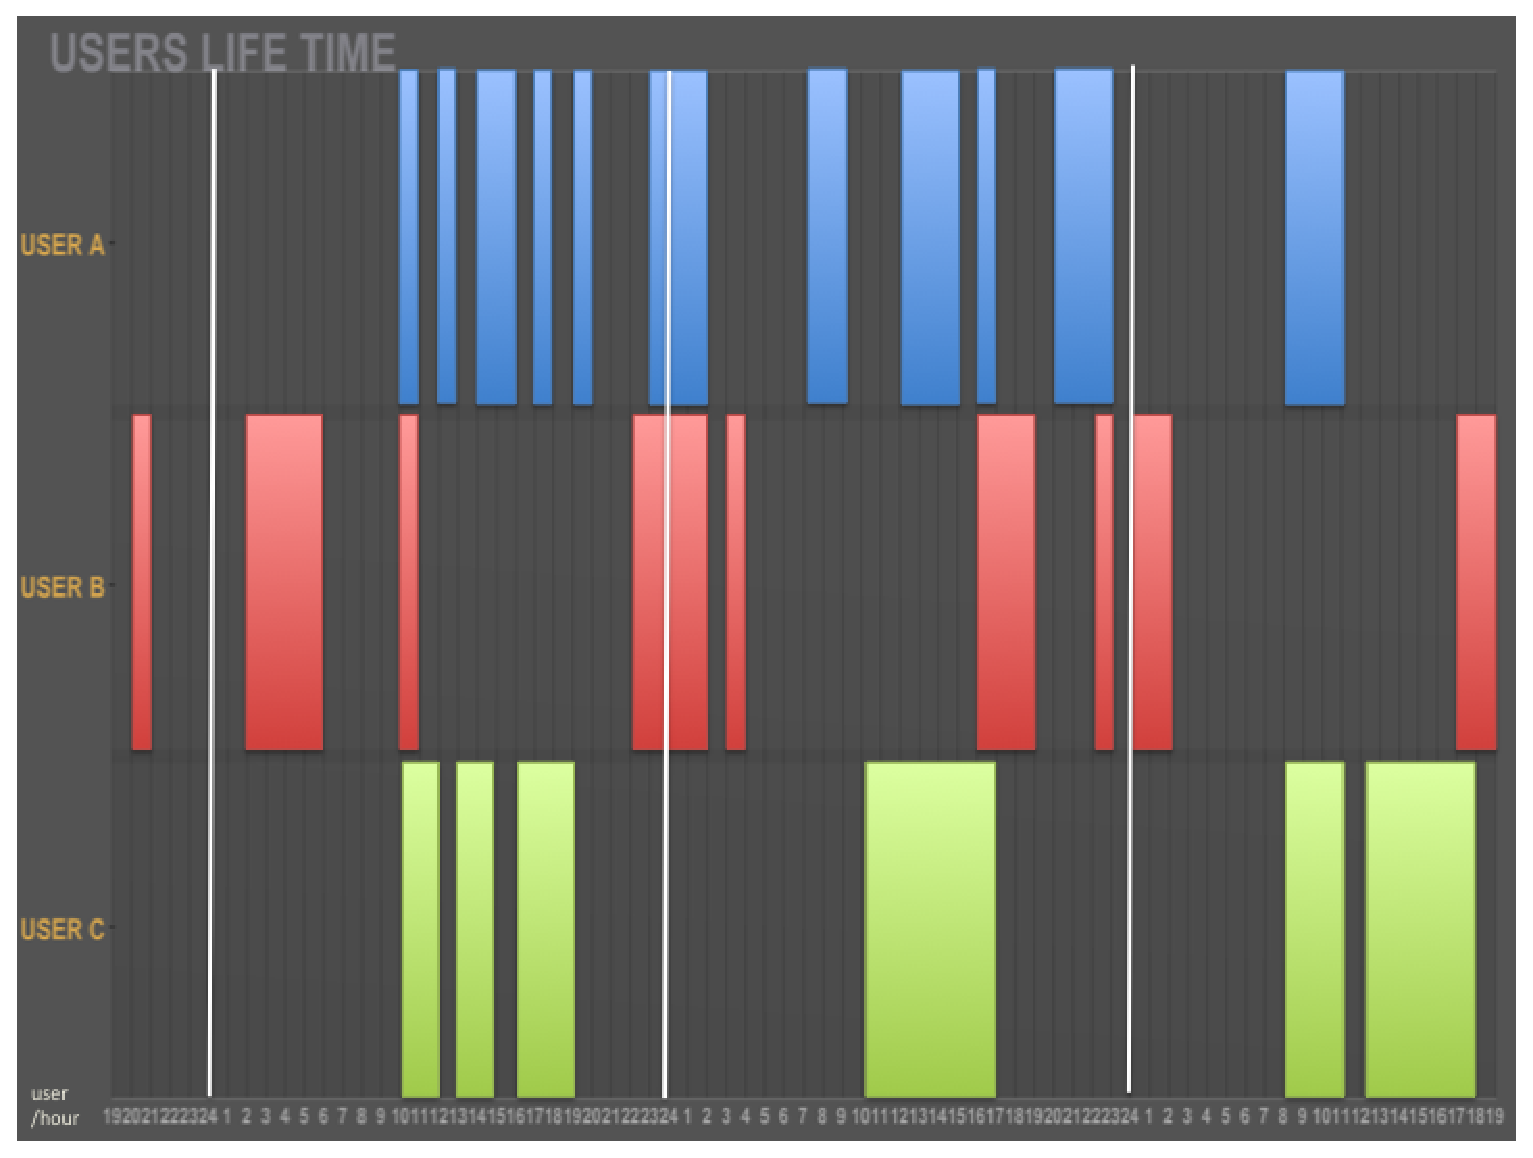
\includegraphics[scale=0.40]{./figure/life_time.eps}
      \caption{��ͭ�ۥ���̾���Ѥ����桼�������ǥ�}
      \label{fig:user_lifemodel}
    \end{center}
\end{figure}

���ˡ���ͭ�ۥ���̾���Ȥˡ��桼������������Ӥ�������뤳�Ȥ��Ǥ�����
��\ref{fig:user_lifemodel}�ˤ��η�̤򼨤������Υ���դϷ�¬���֤�30ʬ
���Ȥ˶�ʬ�����ơ�������֤ǥۥ���A��ȯ�����줿��硤�ۥ���A�ϴ�¬����
�������Ӥϥͥåȥ���ˤ���Ȳ��ꤹ�롥�ץ��ȥ���δط��塤������֤�
�Ȥ˥ꥹ�Ȥξ������Ȥ�򤷤ʤ����ᡤ���μ�ˡ����Ѥ�����

���η�̤��顤��ޤ��ʥ桼��������ꥺ�����ħ��Ƴ���Ф���롥�桼��A��
��˸��漼�˺��Ҥ��Ƥ��ꡤ�����٤Ǹ��Ф���Ƥ��롥���ˡ��桼��B����Τ�
���漼�Ǵ�¬����Ƥ��뤿�ᡤ�뷿����������äƤ��뤳�Ȥ���¬�Ǥ��롥�桼
��B�Ȥϵդ˥桼��C��ī������������äƤ��ꡤ���δ�����ϵ�§����������
����������Ƥ��뤳�Ȥ�ʬ���롥

\subsection{�ͻ�}
��ͭ�ۥ��ȤΥ����ƥ�Ǥϡ��桼���ȥۥ��Ȥ��ӤĤ��뤳�Ȥ��ưפˤʤ뤳
�Ȥ򼨤������ܥ����ƥ�ˤ�äơ�MAC���ɥ쥹�ȶ�ͭ�ۥ���̾�η�ӤĤ���
�뤳�Ȥǡ�ʣ���ۥ��Ȥ����Ѥ��Ƥ�����䡤���롼�פǴ������Ƥ���ۥ���
�ξ��������Ǥ��롥���Υ����ƥ�ˤ�äƥͥåȥ����ǥե����붦ͭ��
���Ѥ��Ƥ���ۥ��Ȥ����꤬��ǽ�Ǥ��뤿�ᡤ�桼���Υץ饤�Х��򶼤�����
ǽ�������˹⤤�ȸ����롥���ξ�����ݻ����Ƥ����ȡ�MAC���ɥ쥹�ȥۥ�
�Ȥ��б���ʬ���뤿�ᡤ�����ФΥ����䡤�ѥ��åȤΥإå�������Ȥ߹�碌
�뤳�Ȥǡ����ܺ٤ʥץ��ե����뤬�����Ǥ��롥�ե����붦ͭ�ץ��ȥ�
���iTunes\cite{iTunes:2009}��Ϥ���Ȥ���¿���Υ��ץꥱ������������
����Ƥ��뤿�ᡤ�������ưפǤ���ȸ����롥

��������NetBIOS��mDNS�Ȥ��ä��ץ��ȥ���ϥ����ӥ������Ѥ��Ƥ��ʤ�����
��������³���Ƥ����礬���뤿�ᡤ�������ͤ��߷פ�Ĵ������ɬ�פ����롥
���������ե����붦ͭ�����Ѥ��Ƥ��ʤ��ۥ��Ȥμ��̤��Բ�ǽ�Ǥ��롥�ޤ���
��ͭ�ץ��ȥ���Ͼ��������³����櫓�ǤϤʤ������Τ��ᡤʬñ�̤ǤΥ桼
����������֤�����Ǥ��ʤ��Ȥ������������롥

\section{Bluetooth�ǥХ���̾}
\label{evaluation:bleutooth}
\subsection{���ڼ�ˡ}
ɮ�Ԥ���°���븦�漼�ˤ����ơ�Bluetooth�򸡽Ф���ץ�������¹Ԥ��뤳�Ȥǡ�
�ɤ����پ�������Ǥ��뤫�򸡾ڤ�����
�ºݤˡ��ڥ���󥰻���Bluetooth���ɥ쥹����������桼���μ�����䵡�����
�Ѥ����ץ��ե�����������ɤ����٤ξ��������Ǥ���Τ��򸡾ڤ�����

\subsection{�߷׳���}
\begin{table}
\begin{center}
\caption{Bluetooth�ǥХ������ɥ쥹���ڼ�ˡ�μ����Ķ�}
  \vspace{5mm}
\label{tb:Bluetooth}
\begin{tabular}{|c|c|c|}
\hline
���͸���&library&OS\\
\hline 
java1.6&Bluecove 2.1.0&MacOSX 10.6.2\\
\hline
PHP&&MacOSX 10.6.2\\
\hline
\end{tabular}
\end{center}
\end{table}
Bluetooth���ɥ쥹�θ��ڼ¸���Ԥ��ץ�������ɽ\ref{tb:Bluetooth}�Ǽ����褦�ˡ�
java����ǵ��Ҥ���MacOSX��Ǽ¹Ԥ��롥
���Ѥ���饤�֥���bluecove 2.1.0�����Ѥ���Bluetooth�ǥХ�����õ����Ԥ���
�ǥХ���õ���Ǹ��Ф�������ϡ���������������Bluetooth���ɥ쥹��Bluetooth�ǥХ���̾�Ǥ��롥
�ǥХ���õ���δֳ֤�30�ä˰��γ���Ϣ³���ƹԤ���
�ǥХ���õ���塤�������������ե�����˽��Ϥ������Ϥ����ե������
PHP�ˤ�륹����ץȤˤ�äơ�����դˤ���в��򤹤롥

\subsection{���ڴĶ�}
���ڴĶ���ɮ�Ԥ���°���븦�漼���������������ϰϤ�ɮ�Ԥμ¸��ۥ��Ȥ���
���Ͽ��᡼�ȥ��ϰϤǤ��롥�ǡ���������������֤ϡ�2009ǯ12��17��23:00��
��2009ǯ12��19��21:00�ޤǤǤ��롥Bluetooth�ǥХ�����õ������ۥ��Ȥ���
�־��ϸ��漼���濴���Ǥ��롥Bluetooth��ͭ���ϰϤϿ�m�����ɴm�ȵ����
�Ķ��ˤ�äƺ������뤿�ᡤ����ǥХ����ˤ�äƤϸ��ФǤ��ʤ���礬��
�롥�����MacBook Pro��ThinkPad T41��2����Ѥ��ơ������˸��ڤ�Ԥä���
���漼�Ͻ�22m����7m�ι����Ǥ��뤬���ɤξ��Ǥ�Bluetooth�ǥХ���������
���줿���ᡤ��ˡ���ڤ�Ԥ�����ܼ¸���������־�������ʤ��Ȥ��롥

\subsection{���ڷ��}

\begin{figure}
    \begin{center}
      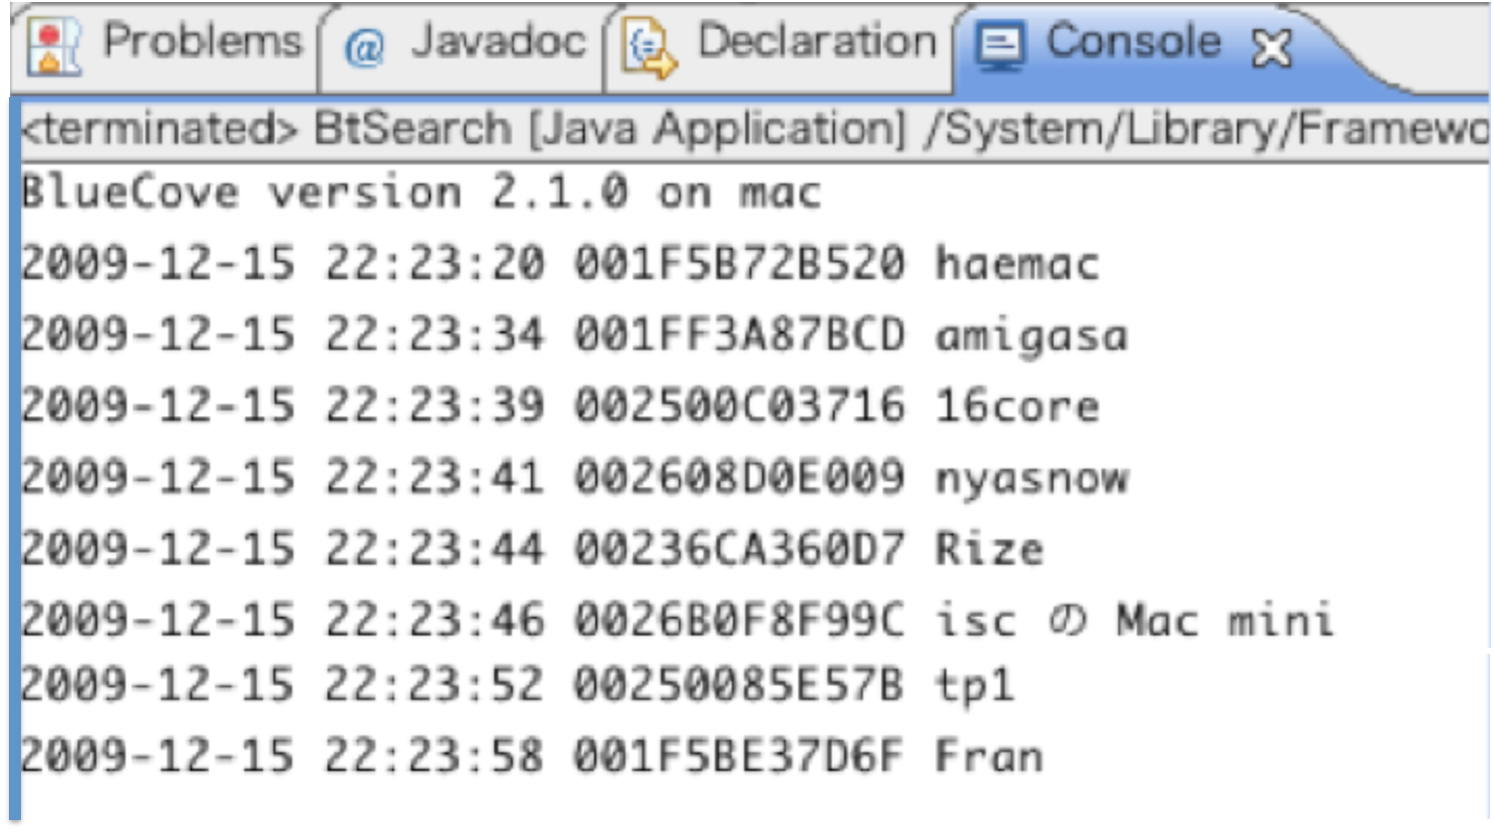
\includegraphics[scale=0.50]{./pdf/Bluetooth_display}
      \caption{Bluetooth�ǥХ����θ���}
      \label{fig:track_con}
    \end{center}
\end{figure}

\begin{table}
\begin{center}
\caption{Bluetooth�ǥХ������ɥ쥹���ڷ��}
  \vspace{5mm}
\label{tb:Bluetooth_res}
\begin{tabular}{|c|c|c|c|}
\hline
ȯ���ۥ��ȿ�&����ۥ��ȿ�&����ü����\\
\hline 
26&5&3\\
\hline
\end{tabular}
\end{center}
\end{table}



�嵭�Υץ�������¹Ԥ����Ȥ�����\ref{fig:track_con}�Τ褦�ʾ�������������
�����Ǽ����Ǥ�������Bluetooth�ǥХ������ɥ쥹�ȼ������֡����ꤷ�Ƥ���Bluetooth�ǥХ���̾�Ǥ��롥
��ͭ̾��Ʊ������MacOSX�����Ѥ��Ƥ��ꡤ���ĥǥե���Ȥ�����򤷤Ƥ��ʤ�����
��ͭ�Ԥȥۥ��Ȥε���̾��ɽ��������̤ˤʤä���

���ˡ����������ǡ�������Ϥ�����̤�ɽ\ref{tb:Bluetooth_res}�˼�����
���ڴ�����˼�������Bluetooth���ɥ쥹��������26���ä���
��\ref{background:user_in_network}��Ǥϡ����θ��漼��100��᤯��
�ۥ��Ȥ����뤳�Ȥ򼨤��Ƥ��뤿�ᡤBluetooth�����Ѥ��Ƥ���ۥ��Ȥ����Ū
���ʤ��Ȥ����롥������ǡ�24���־�˲�Ư���Ƥ���ۥ���5��ȯ�����줿����
���ϥ����ФȤ������Ѥ���Ƥ����ǽ�����⤤�����ˡ��ۥ��ȤǤϤʤ����ޡ�
�ȥե���Ȼפ��뵡�郎3�Ĵ�¬����Ƥ��롥�ޤ�����ͭ�ۥ���̾��ɽ������
�������Ȥˡ��ۥ��ȴ֤δط�����¬���Ǥ��롥�����¬���줿����
�顤Bluetooth�ǥХ���̾��Ʊ�����郎3�Ȥ��ä������Τ����ҤȤ��3��Υۥ��Ȥ�����
���Ƥ���桼���䡤���롼�פǴ�������Ƥ���ۥ��ȷ�����¬���줿�����Τ�
���ˡ�Bluetooth�ǥХ���̾�����Ѥ�������ǥ桼���䥰�롼�פ��ɤΤ��餤�Υۥ��Ȥ�
���Ѥ��Ƥ���Τ���¬�Ǥ��롥

�ޤ���Bluetooth���ɥ쥹�ϸ�ͭ�Τ�ΤǤ��ꡤ�ۥ���̾�ȥХ���ɤ��뤳�Ȥˤ�äơ�
��ͭ�ۥ���̾��Ʊ���褦�ˡ�������֤���Υȥ�å��󥰤���ǽ�Ȥʤ롥
��\ref{fig:Bluetooth_track_life}�˼�����������ˤ�äƺ�����������դ�
���������Υ���դκ����⡤��\ref{fig:user_lifemodel}��Ʊ������ˡ�Ǻ�����
����Bluetooth�ǥХ��������Ͼ���Ԥ��뤿�ᡤϢ³���Ƽ������뤳
�Ȥ��Ǥ��뤿�ᡤ5ʬ��˶�ʬ��������¬���줿�����Ӥϼ�������μ��դ˥桼���������ΤȤ��롥

���θ��ڤǤϡ�����Ū�˻����⤭���Ƥ���桼���Υۥ��Ȥ�3�������ӽФ�����
3�ͤΥ桼������ħ���ФƤ��롥�桼��A��B�����Ū�뷿�η��������뤳�Ȥ��Ф��ơ�
�桼��C����˸��漼��ˬ��Ƥ��롥
�ޤ������θ��ڤ������������������ˤ����ƹԤäƤ��뤿�ᡤ�ɤΥ桼��
����������ͼ���ޤǸ��漼��ˬ��Ƥʤ����Ȥ�ʬ���롥

\begin{figure}
    \begin{center}
      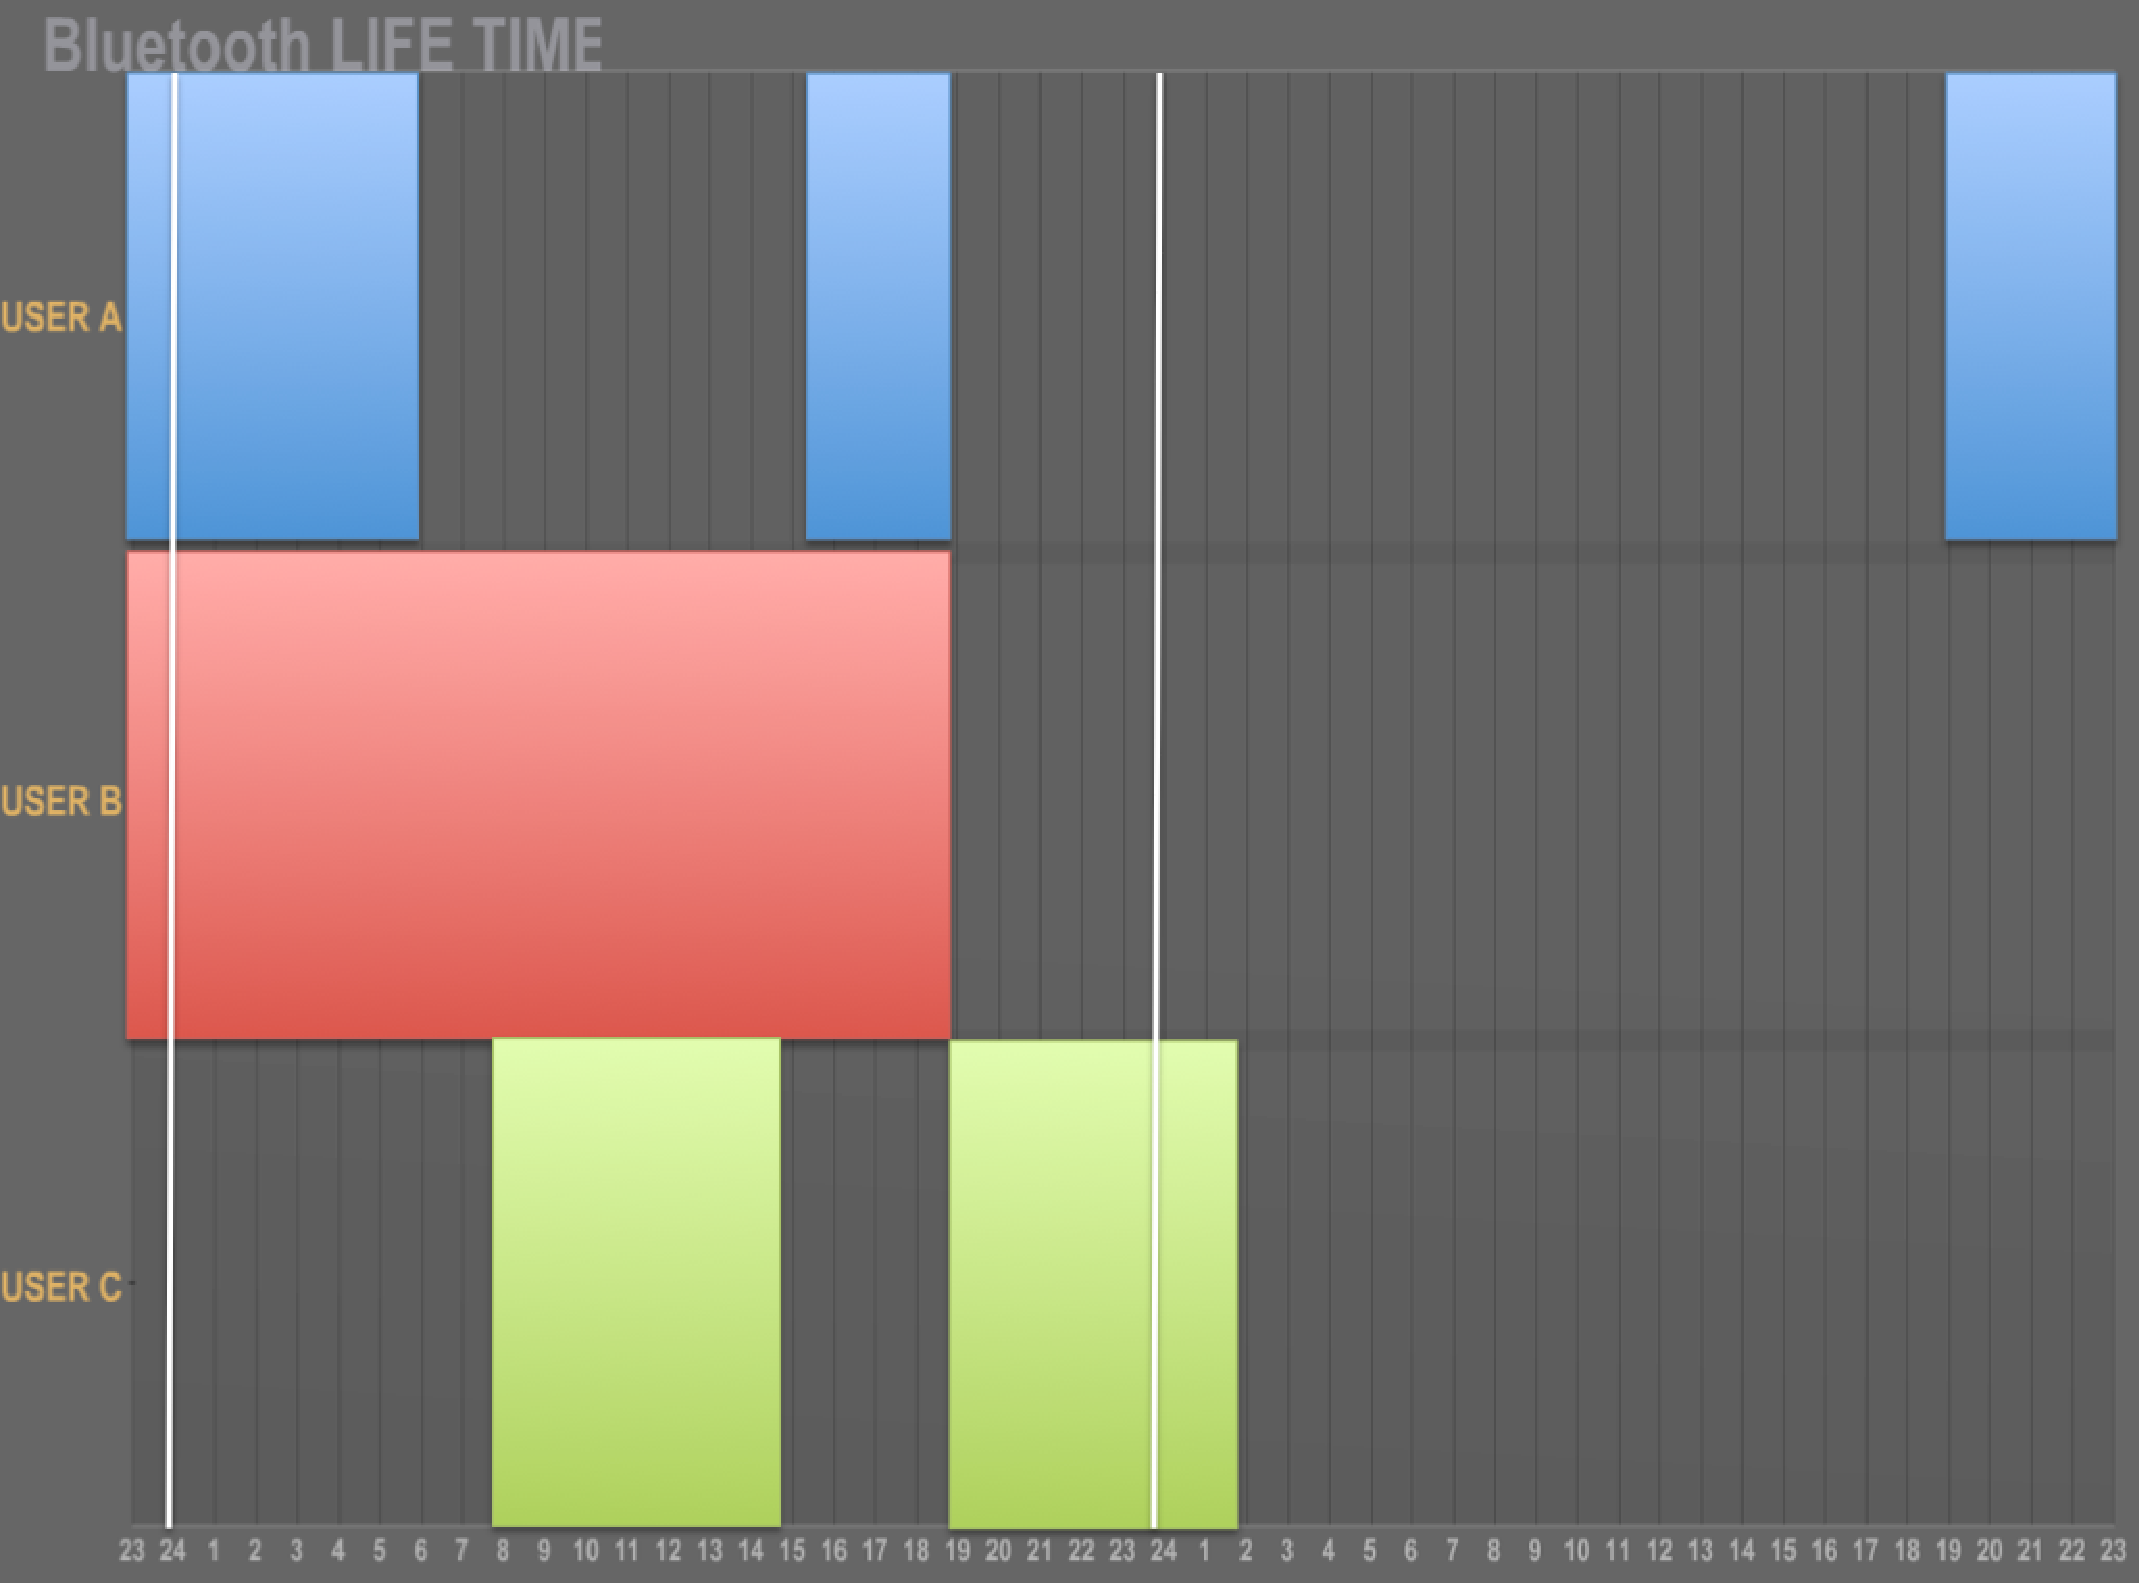
\includegraphics[scale=0.35]{./pdf/Bluetooth_lifetime}
      \caption{Bluetooth�ǥХ����θ��Фˤ��桼���Υ饤�ե�����}
      \label{fig:Bluetooth_track_life}
    \end{center}
\end{figure}

\subsection{�ͻ�}
Bluetooth�Υ����ƥ�����Ѥ�����̡�Bluetooth�ǥХ���̾��Bluetooth���ɥ쥹�����
���뤳�Ȥ��Ǥ��������Υ����ƥ����Ѥ��뤳�Ȥˤ�äơ��桼���ξ�����
����֤�������뤳�Ȥ��Ǥ��롥�桼���ξ��ϡ��ܥ����ƥ���͡��ʾ���
���֤��뤳�Ȥˤ�äƸ��в�ǽ�Ǥ��롥�ܥ����ƥ�Ǥ�30�ä�1�٥ǥХ���õ��
�򤹤뤿�ᡤ��ͭ�ۥ���̾�Υ����ƥ�����ưפ������Τ˼����Ǥ��롥����
���åȤ������Ǥ��ꡤ���־�꤬���漼�������ꤹ��ȡ��桼�������Ф����
���ä����֤ιֵ��䥤�٥�Ȥ�õ�����Ȥǡ��桼�����ɤ��ˤ���Τ����¬��
�뤳�Ȥ�Ǥ��롥���Τ��Ȥ��顤Bluetooth�ϥ桼���ץ饤�Х��򶼤�����
ǽ��������Ȥ����롥Bluetooth�ǥХ���̾�����ꤷ�Ƥ��ʤ����ϥ桼��̾��OS̾�Ȥ�
�롥���Τ��ᡤ��ͭ�ۥ���̾�Υ����ƥ��Ϣư���뤳�Ȥǡ�MAC���ɥ쥹���ۥ�
��̾��Bluetooth���ɥ쥹��3�Ĥ��ӤĤ��뤳�Ȥ��Ǥ��롥�����ơ���ӤĤ�
��MAC���ɥ쥹���鶦ͭ�ۥ��Ȥ�Ʊ���褦��¿���μ������Ǥȷ�ӤĤ��뤳�Ȥǡ�
�桼���Υץ��ե����뤬��ǽ�Ȥʤ롥���ڤξϤǤ�Ҥ٤��褦�ˡ�Bluetooth��
���Ѥ���桼����¿���Ȥϸ����ʤ����������Bluetooth����ڼ���ˤ�äƤ�
���˶��Ϥʼ������ǤȤʤ롥��������Bluetooth�ΥǥХ���õ���ϡ��桼����
õ���򤷤������ˤΤ����Ѥ���Τ�����Ū�Ǥ��뤬���¸���̤���ڹ�����
Ĵ���ǵ󤲤Ƥ���褦�˾��õ���򤷤Ƥ���ǥХ�������¿�����뤳�Ȥ�ʬ
���롥���õ����ͭ���ʵ�ǽ�Ǥ��뤫�ϵ�����ɬ�פǤ��롥

\section{���ڤ������������}
Bluetooth�ǥХ���̾����ͭ�ۥ���̾���ѥ��åȤΥإå���������礹�뤳�Ȥ�
��äơ�������ΤʸĿͤ����ꤹ�뤳�Ȥ��Ǥ��롥
���ڤ�����줿�����ɽ\ref{tb:combine_info}�˼�����

\begin{table}
\begin{center}
\caption{���ڤ����Ѥ�������}
  \vspace{5mm}
\label{tb:combine_info}
{\footnotesize
\begin{tabular}{|c|c|c|c|}
\hline
���Ѿ���&�ѥ��åȥإå�����&��ͭ�ۥ���̾&Bluetooth�ǥХ���̾\\
\hline
\hline
��դ˥ۥ��Ȥ�&�ʤ�&MAC���ɥ쥹&Bluetooth\\
���̤Ǥ������&&&�ǥХ������ɥ쥹\\
\hline
�ۥ��Ȥο�¬��&�ѥ��åȤΥإå�����&��ͭ�ۥ���̾&Bluetooth�ǥХ���̾\\
���ѤǤ������&�ۥ��Ⱦ���&���־���&���־���\\
&���ѥ����ӥ�&��³����&����ꥺ��\\
\hline
\end{tabular}
}
\end{center}
\end{table}

���ڤη�̡��ġ��ξ��������ˡ����ۥ��Ȥξ�������Ǥʤ����ۥ��Ȥ��ͭ��
�ξ��������Ǥ��뤳�Ȥ�ʬ���ä��������ǡ��ѥ��åȤΥإå����󡤶�ͭ��
����̾��Bluetooth�ξ�����Ȥ߹�碌�륷���ƥ��ISP��ͥåȥ��������
�����Ѥ�����硤�桼�������ꤵ����ǽ����ͻ����롥�ܼ�ˡ�Ǥϡ��ѥ���
�ȤΥإå�����Ȥ��η��������Ѥ��ƥץ��ե������������롥���Τ�
�ᡤISP�Τ褦���絬�ϥͥåȥ���ˤ����ơ��ѥ��åȤΥإå�����Ȥ��ä�
�������ǤΤߤǤϥ桼���Υץ��ե����뤬����Ǥ��롥�������Ǥˤϡ���ͭ�ۥ���
̾�䡤Bluetooth�ΥǥХ������ɥ쥹�⼱�����ǤȤ������Ѳ�ǽ�Ǥ��롥�ѥ��å�
�Υإå���������Ǥϡ��桼���ο����񤤤ˤ�äơ��ۥ��ȼ��̤����٤��Ѳ�
���롥����������ͭ�ۥ���̾��MAC���ɥ쥹��Bluetooth�ΥǥХ������ɥ쥹��
�Ȥ߹�碌��������ݻ����뤳�Ȥǡ���郎�����Х桼�����ۥ��Ȥ�ʣ������
�Ƥ������䡤�ۥ��Ȥ��Ѥ��Ƥ����פ���ǽ�Ǥ��롥�ǽ�Ū�ˤϡ��ۥ��Ȥȷ�
�����äʤɤε�����Ȥ߹�碌���ͥåȥ���˷Ҥ��뤹�٤Ƥε���
�ȡ�Bluetooth�����ѤǤ��뵡����ӤĤ��ƥץ��ե����뤹�뤳�Ȥ��Ǥ��롥
�����ơ��Ƶ��狼�顤�¥桼���ΰ��֡����֡���ư�����Ȥ��ä��Ŀͤ˴ؤ��
�����ܿͤ��Τ�ʤ��֤����Ѥ��������������롥


%\subsection{�桼�������ꤵ�����}
%�ºݤˤɤΤ褦�ʾ�����Ȥ߹�碌��ȥ桼��������ˤĤʤ���Τ���ͻ����롥
%�桼�������ꤹ����ϥѥ��åȤΥإå�����ȶ�ͭ�ۥ���̾�ˤ�ä�����Ǥ��롥
%�ۥ��Ⱦ���ȶ�ͭ�ۥ���̾�ˤ�äƤϾ����ưפ˼����Ǥ��롥
%ɽ\ref{tb:combine_info}�˵����������Ƥ��Ȥ߹�碌�뤳�Ȥ�¿���Τ��Ȥ�ʬ���롥
%�äˡ�MAC���ɥ쥹�������Ǥ�����礬�����Ǥ��롥
%
%\subsection{�桼�������ꤵ����ǽ����������}
%\subsection{�桼�������ꤵ��ʤ�}
%


�ʾ�Τ��Ȥ���ѥ��åȤΥإå����󡤶�ͭ�ۥ���̾��Bluetooth�ǥХ����ϡ��桼����ȥ��
���󥰤���ˤ����ꡤ����ͭ���ʼ��ʤǤ���ȤȤ�ˡ��桼���Υץ饤�Х�
�˶��Ҥ�Ϳ�����ΤǤ���ȸ����롥



\section{�ޤȤ�}
�ܾϤǤ�3�Ĥβ���򸡾ڤ������ѥ��åȤΥإå�����ȡ���ͭ�ۥ���
̾��Bluetooth�ˤ��ۥ��ȼ��̤β�ǽ���Ǥ��롥�ѥ��åȤΥإå�����Τߤ�
�Ѥ��ơ��ۥ��Ȥ��̤����ˡ�ϡ��ͥåȥ����������������֤������Ū
�˥إå�����Τߤ���������������Ǥ��Ȥ˥ۥ��Ȥ�ʬ�ह�롥����ˤ�äơ�
�ͥåȥ����Υۥ���7��Τ���4����̤��뤳�Ȥ��Ǥ��������ˡ���ͭ��
����̾��Bluetooth���ɥ쥹�ϥۥ��Ȥȥ桼��̾��ǥե���Ȥ����ꤷ�Ƥ���ȥ桼��
�����Ѥ��Ƥ���ۥ��Ȥ�桼�����Ȥ�����ο�¬����ǽ�ˤʤ뤳�Ȥ򼨤�����
�����3�Ĥξ���ϡ��桼���Υץ饤�Х��򶼤�����ǽ������ʬ�ˤ���ȸ���
�롥
%%% Local Variables:
%%% mode: japanese-latex
%%% TeX-master: "../nakajima_bthesis"
%%% End:


\chapter{�����ɥ饤������}
\label{consideration}
�ܾϤǤ���\ref{evaluation}�ϤǤθ��ڷ�̤��Ȥˡ������ɥ饤�����Ƥ�
���������ɥ饤��ϰ��̥桼���ȳ�ȯ������Ԥ�ʬ������Ƥ��롥�ѥ��åȤ�
�إå����󡤶�ͭ�ۥ���̾��Bluetooth�ǥХ���̾�ϥ桼���Υץ饤�Х��򶼤�
����ǽ�������뤳�Ȥ����Ҥ����̤�Ǥ��롥�������������ӥ�������뤿���
�ϡ������ξ�������Ѥ��ʤ���Фʤ�ʤ��������ǡ������ξ���򰷤���
�Υ����ɥ饤�����Ƥ��롥�����ɥ饤����оݤϼ�ˡ����̥桼������ȯ�ԡ�
�����ԤǤ��롥

\section{���̥桼���Υ����ɥ饤��}
\label{conclusion:guide}
\begin{figure}
  \begin{screen}
    \begin{itemize}
    \item �ǥե��������γ�ǧ\\
      ������ü�����ܿ����ꤷ�Ƥ��ʤ��Τ˴ؤ�餺���������Ǥ�ȯ�����Ƥ���
      ��礬����Τǡ�������ǧ���롥
    \item ��Ū�Ȥ������ʳ��Ǥϥ����ӥ������Ѥ��ʤ�\\
      �������ӥ������Ѥ��Ƥ��ʤ����ϡ������ӥ��˴ؤ�뵡ǽ��Ȥ�ʤ���
    \item ���Ȥ����Ѥ��륵���ӥ��ο����٤γ�ǧ\\
      �������ӥ���������硤�Ŀ;��������������꤬���ɤΤ褦��
      ���������򤷤Ƥ��뤫��ǧ���롥
    \item ���Ѿ���γ�ǧ\\
      �������ӥ�������뤿��ˡ�ȯ������������꤬�ʤ������ǧ���롥
    \end{itemize}
  \end{screen}
  \caption{���̥桼���Υ����ɥ饤��}
  \label{itembox:user_guidline}
\end{figure}

�ǥ�����ǥХ������������äˤ����ơ����̥桼���Υץ饤�Х��ݸ������
���ϥȥ졼�ɥ��դ�¦�̤����롥�äˡ��桼���Υץ饤�Х��ϥ桼�����Ȥ��
��ɬ�פ����뤿�ᡤ�桼�����ȤΥ����ɥ饤��ɬ�פȤʤ롥���̥桼���ξ�
��Υ����ɥ饤����\ref{itembox:user_guidline}�˼�����

�ޤ����桼�������ꤹ�뼱�����ǤȤʤ�ǥХ���õ����ǽ�ϥǥե���Ȥǥ���
�ˤ������õ���򤷤ʤ��������ӥ����������ʳ������Ѥ��ʤ��褦���ꤹ
�롥����ϡ�Bluetooth�ΥǥХ���̾�ǵ󤲤���褦�ˡ��桼�����տޤ�����
���Ȥξ������Ϥ�ȯ�����Ƥ����礬���뤿��Ǥ��롥

���ˡ���ͭ�μ������Ǥ����Ѥ��륵���ӥ��Ǥϡ����ѻ��ʳ��ϻ��Ѥ��ʤ�����
�����פǤ��롥�����ӥ����ѻ��ʳ��ˤ��ε�������Ѥ��ʤ����Ȥϡ����Ϥ˼�
�Ȥξ����ȯ������������򸺤餹���ȤˤĤʤ��뤿��Ǥ��롥

�����ơ��桼���ϥ����ӥ����ѻ��ˤ����ơ��ɤΤ褦�ʾ������Ѥ���Ƥ���
�����ǧ�����桼�����Ȥ����Ѥ��Ƥ��뵡��Υ����ӥ����İ�����ɬ�פ����롥
���Ȥ�ȯ�����Ƥ��������Τ뤳�Ȥǡ��桼���Υץ饤�Х��˴ؤ�뤫�ɤ���Ƚ
�Ǥ��뤳�Ȥ��Ǥ��롥�ޤ��������ӥ��������ˤ����ꡤ�桼���ξ�������
����褬����Ǥ��뤫�ɤ������ǧ���ʤ���Фʤ�ʤ����㤨�С��Ŀ;���μ�갷��
�δ����������Ƥ��뤫�ʤɤǤ��롥

�����Υ����ɥ饤����뤳�Ȥˤ�äƥ桼���ϼ��ȤΥץ�Х����ݸ��
���Ȥ��Ǥ���ȸ����롥�桼�����Ȥ�ȯ�����Ƥ��������Τꡤȯ���������
��桼�������뤳�Ȥǡ��桼���Υץ饤�Х�������������ǽ�����㸺����
���Ȥ��Ǥ��롥


\section{��ȯ�ԡ������ԤΥ����ɥ饤��}
��ȯ�Ԥ�ͥåȥ�������ԤΥ����ɥ饤����\ref{itembox:guidline}�˽Ҥ٤롥

\begin{figure}
  \begin{screen}
    \begin{itemize}
    \item ��������ˤ�����桼����Ʊ��\\
      �ѥ��åȾ���ȥۥ���̾�Ȥ��ä�ʣ���θĿ;�����Ѥ���
      ���ϡ�ɬ���桼����Ʊ�դ����롥���뤳�Ȥ�����ʾ��ϻ����˳��פ���
      ���������ץȥ����ȷ�������ѡ�
    \item �桼���ˤ�����Ѿ��������\\
      �ɤ��ޤǤξ�������Ѥ����ɤ��Τ���桼�����������롥
    \item ���Ѽ������Ǥθ���\\
      ������Ȥ߹�碌���硤Mac���ɥ쥹�ʤɥۥ��Ȥ��դ�����Ǥ����ѹ���
      ����Ǥ��뼱�����Ǥ����Ѥ��ʤ���
    \item ������\\
      �Ŀ;�����������ݤϡ����ξ�������Ѥ���Τ��������Ȥ߹�碌��Τ���
      ���η�̡��ɤ��������󤬼����Ǥ���Τ������Τˤ���
    \item �桼���ˤ��������\\
      �桼���˼������Ǥ���Ϳ�⤷�������Ѥ�����ϡ��桼��¦���ưפ˼���
      �Ҥ��ѹ�������Ȥ��ä������Ǥ���褦�ˤ��롥
    \item ϳ�̻����к�������\\
      �桼���μ������Ǥ�ή�Ф��Ƥ��ޤä������к�����������ɬ������
    \end{itemize}
  \end{screen}
  \caption{��ȯ�ԡ��ͥåȥ�������ԤΥ����ɥ饤��}
  \label{itembox:guidline}
\end{figure}

��\ref{background}�ϤǽҤ٤��褦�ˡ��桼���˴ط������������Ѥ����
��ϥ桼����Ʊ�դ�ɬ�פǤ��롥�桼����Ʊ�դʤ��˾���μ�������Ѥ�Ԥ�
����硤�ץ饤�Х��򿯳������ǽ�������롥������夲��3�Ĥξ���ϥץ�
���Х��򶼤������ᡤ�������������Ѥ�����ϻ�����Ʊ�դ����롤�⤷��
�ϥ��ץȥ����Ȥη�����Τ뤳�Ȥ�˾�ޤ�������������NebuAd�Ǥλ���Τ褦
�ˡ�ˡΧ�˿���Ƥ��ʤ��Τˤ�ؤ�餺���桼����ץ��Х����������������
�뤳�Ȥ�ɱ󤹤뤳�Ȥ����롥���Τ��ᡤ�桼���������ӥ��󶡼�����������
�Τ���ˡ������ξ�������Ѥ���ݤϡ��桼����Ʊ�դ����뤳�Ȥ�ɬ�פǤ�
�롥�ޤ��������ξ����MAC���ɥ쥹�Τ褦�ʰ�����ζ�������ȷ�ӤĤ���
��硤�Ŀͤ����ꤵ��䤹�����ᡤ�ץ饤�Х��ݸ�δ��������ӤĤ��ƤϤ�
��ʤ���MAC���ɥ쥹�����Ѥ��뤳�Ȥǡ�¿���ξ�����ӤĤ��뤳�Ȥ��Ǥ���
�Τ���\ref{consideration}�Ϥ���Ƭ�ǽҤ٤��̤�Ǥ��롥

�桼�����������Ǥ�������������ǥ����Ǥ�󤲤��褦�ˡ��������Ǥ�
����˽ऺ���Τ�桼������Ϳ�����硤�桼�������ȤǾ����ȯ������
������Ǥϡ�Ʊ�դΤۤ��ˤ⡤�ưפ˴����Ǥ��뤳�Ȥ�ɬ�ܤǤ��롥�ޤ���
�桼�����Ȥ�ȯ���Ƥ������������ǤȤ��ƻ��Ѥ�����ϡ����ξ����桼
�����Ȥ������Ǥ���褦�˹��Τ��뤳�Ȥ���Ƥ��롥

�ܥ����ɥ饤��ǺǤ���פ����ϡ�����������Ԥ�����������Ū����̤�
��ʸ�����桼����Ʊ�դ����뤳�Ȥȡ��������ǤȤʤ����ϡ��桼�����Ȥ���
ͳ�˴����Ǥ���褦�˾�����󶡤��뤳�Ȥ�2���Ǥ��롥

\section{�����ɥ饤��ν�­�٤θ�Ƥ}
���Ҥ��������ɥ饤��ˤ����뽼­�٤�Ƥ���롥�ޤ����桼���Υ����ɥ饤
��ˤĤ��ƽҤ٤롥�桼�������Ѥ��뵡��ϥץ饤�Х�����θ����Ƥ���ɬ��
�����뤬�������ӥ�������뤿��ˤϡ����Ȥξ����ȯ�����ʤ���Ф����ʤ�
��礬���ꡤ�������ȥץ饤�Х��Υȥ졼�ɥ��դǤ��롥����ϥ桼�����Ȥ�
�����ӥ������Ѥ�����������򤷡�Ʊ�դ򤹤�Ȥ����԰٤˽Ť����������
���Ȥ�ͽ�ۤ���롥���Τ���ˤ⡤�桼���ΰռ�������Բķ�Ǥ��뤿�ᡤ��
�����ɥ饤��Ǥ϶�Ĵ���Ƥ��롥

�����ԡ���ȯ�ԤΥ����ɥ饤��ν�­�٤�OECD8��§\cite{OECD8:1980}����
�˽�­�٤�Ƥ���롥OECD8��§�ϡ�1980ǯ��OECD�˺��򤵤줿�Ŀ;����ݸ��
�ؤ�����Ū�ʥ����ɥ饤��Ǥ��롥OECD8��§���\ref{itembox:oecd}�˼�
����OECD8��§������ʸ���󼨤��륬���ɥ饤�����Ӥ����б�������̤�
ɽ\ref{tb:guidline}�˵�����

\begin{figure}
  \begin{screen}
    \begin{description}
    \item 1 �������¤θ�§\\ 
      �Ŀͥǡ����ϡ�Ŭˡ�������ʼ��ʤˤ�ꡤ���ľ�����Τ����Τޤ���Ʊ
      �դ����Ƽ��������٤��Ǥ��롥
    \item 2 �ǡ������Ƥθ�§\\
      ��������ǡ����ϡ�������Ū�˱�ä���Τǡ����ġ����Ρ��������ǿ��Ǥ�
      ��٤��Ǥ��롥
    \item 3 ��Ū���β��θ�§\\
      ������Ū�����Τˤ����ǡ������Ѥϼ�����Ū�˹��פ���٤��Ǥ��롥
    \item 4 �������¤θ�§\\
      �ǡ������Τ�Ʊ�դ��������ˡΧ�ε���ˤ���������ơ����������ǡ�
      ������Ū�ʳ������Ѥ��ƤϤʤ�ʤ���
    \item 5 �����ݸ�θ�§\\ 
      ����Ū�����ݸ����֤ˤ�ꡤʶ�����˲������ѡ������������������ݸ�
      ���٤��Ǥ��롥
    \item 6 ������\\ 
      �ǡ��������μ»�����������������ǡ�����¸�ߡ�������Ū����������
      ����������٤��Ǥ��롥
    \item 7 �Ŀͻ��äθ�§\\ 
      �ǡ������Τ��Ф��ơ����ʤ˴ؤ���ǡ����ν�ߵڤ����Ƥ��ǧ������
      �ޤ��ϰ۵Ŀ�Ω���ݾڤ���٤��Ǥ��롥
    \item 8 ��Ǥ�θ�§\\ 
      �ǡ����δ����ԤϽ���§�»ܤ���Ǥ��ͭ���롥
    \end{description}
    \end{screen}
  \caption{OECD8��§}
  \label{itembox:oecd}
\end{figure}


\begin{table}
\begin{center}
\caption{�����ɥ饤��ν�­��}
\label{tb:guidline}
\begin{tabular}{|c|c|c|}
\hline
�����ɥ饤�� & �б�����OECD8��§&����\\
\hline
�桼����Ʊ�� &1,2,3,4&\\
\hline
�桼�������Ѿ�������&1&\\
\hline
�������Ǥθ���&&������ʤ�\\
\hline
������&2,3,4,8&\\
\hline
�桼���ˤ��������&7&\\
\hline
ϳ�̻����к�������&5,6&\\
\hline
\end{tabular}
\end{center}
\end{table}

�ޤ����桼����Ʊ�դ˴ؤ�����ܤϡ�OECD8��§��1���������¤θ�§���ǡ���
���Ƥθ�§����Ū���β��θ�§���������¤θ�§�Ȱ��פ��롥�桼����Ʊ�դ�
���뤳�Ȥϡ���������ˤ����ƤϤʤ��ƤϤʤ�ʤ�����Ǥ��롥���ˡ��桼��
�����Ѿ��������ϡ��桼����Ʊ�դ�����Ǥ��ꡤƱ�դ��ʤ����ϼ�������
���Ȥ������˰��פ��롥����Ū�˥����ӥ��ϥ桼���Υ��ץȥ��������Ȥ�
���Ȥ�˾�ޤ����������ơ��������Ǥθ���˴ؤ��Ƥϡ�OECD8��§�˳������뵭
�ҤϤʤ������������桼���Υץ饤�Х����ݸ����θ���뤿��ˤ�ɬ�פǤ���
�ȸ����롥����θ����˴ؤ��Ƥϡ�OECD�Υǡ������Ƥθ�§����Ū���β��θ�
§���������¤θ�§����Ǥ�θ�§�˰��פ��롥���ξ�������Ѥ��ơ��ɤΤ褦
�ʾ���ʬ����Τ������β����뤳�Ȥϥ桼����Ʊ�դȤ�Ĥʤ��뤿��ɬ����
�ķ�Ǥ��롥�桼���ˤ���������ϸĿͻ��äθ�§�Ȱ��פ��롥�ä˰۵Ŀ�
��Ω�Ƥ�ꡤ�桼�����Ȥ����Ĥ����ʤ���Ǥ����������Ǥ���褦�˴���
�Ǥ����ǥ뤬˾�ޤ�����ϳ�̻����к��������ϡ������ݸ�θ�§�������θ�
§�Ȱ��פ��롥�ɤΤ褦�˼��Τ������ǤϤʤ���ϳ�̻����к��ˤĤ�������
����٤��Ǥ��롥

���Τ褦�ˡ��ץ饤�Х��Υ����ɥ饤��Ȥ��줿OECD8��§�ˤ����ơ����٤�
�ξ��������������ǤϤʤ������������Ǥ��������Ǥ��뤿�ὼ­�٤�����
���Ƥ���ȸ����롥


%\section{�ץ饤�Х��ݸ�}
%�桼���Υץ饤�Х������硤Bluetooth�䶦ͭ�ۥ��ȤȤ��ä����Ȥ�ȯ����
%�Ƥ����������򤹤�ɬ�פ����롥�ޤ������Ȥ����Ѥ��Ƥ��ʤ����ϡ�����
%�ӥ��˴ؤ��륢�ץꥱ������������򤹤�ɬ�פ����롥���塤�͡��ʥǥ���
%��������Ѥ���븽���ˤ����ơ�����򰷤�¦�����ǤϤʤ����桼���ϼ���
%�ǥץ饤�Х�����ɬ�פ����롥�ɤΤ褦�ʼ������Ǥ����Ѥ����Τ����Τ뤿
%��ˤ⡤����¦��������������뤳�Ȥǡ��桼�����ȤΥץ饤�Х��˴ؤ��뼱
%�̻Ҥؤδؿ����ޤ롥���Τ褦�ˡ��ץ饤�Х����ݸ�뤿��ˤϡ����Ѽ�
%¦�������ӥ�������ƥ���¦��ξ���ι�դ�ɬ�פ��Ǥ��롥

\section{�ޤȤ�}
���̥桼���Υץ饤�Х����ݸ�뤿��ˡ��Ŀ;�����갷���˴ؤ��륬��
�ɥ饤���桼���ȥͥåȥ�������ԡ���ȯ�Ԥ��оݤ�ʬ������Ƥ�������
�̥桼�������Υ����ɥ饤��ϡ��桼�����Ȥ�ȯ���������ˤĤ������򤷡�
��������ɬ�����ˤĤ��Ƥι��ܤ��ߤ��������ˡ������ԡ���ȯ�Ը����Υ�����
�饤��ˤϡ��桼����Ʊ�դ����뤳�Ȥȡ��桼������ͳ�˴������뤳�Ȥ˽���
���֤������ܤ��ߤ����������ơ��ܥ����ɥ饤��ν�­�٤ˤĤ��ƹ��ܤ��Ȥ�
��Ƥ���ͻ�������

%%% Local Variables:
%%% mode: japanese-latex
%%% TeX-master: "../nakajima_bthesis"
%%% End:

\chapter{����}
\label{conclusion}

\section{�ޤȤ�}
\label{conclusion:matome}

\section{�����Ÿ˾}
\label{conclusion:matome}

%%% Local Variables:
%%% mode: japanese-latex
%%% TeX-master: "../nakajima_bthesis"
%%% End:

\chapter*{�ռ�}
\addcontentsline{toc}{chapter}{�ռ�}
\label{thanks}
����ʸ�κ����ˤ����ꡤ����Ƴĺ�������������شĶ������������
Ĺ ¼�� ����Ρ�Ʊ�������� ���� �ѹ���Ρ�Ʊ�������� ��¼ ����Ρ�Ʊ����
�ڶ��� ���� ��Ƿ��Ρ�Ʊ�����ڶ��� �⼮ �쵪��Ρ�Ʊ�����ڶ��� ���� ��
��Ρ�Ʊ�����ڶ��� ���� ������Ρ�Ʊ������Ǥ�ֻ� �Ŷ� �Ϲ���Ρ�Ʊ����
��Ǥ�ֻ� ��߷ ����Ρ�Ʊ������Ǥ�ֻ� Rodney D.Van Meter III ��Ρ�Ʊ��
������ ���� ������Ρ�Ʊ���DMC������Ǥ�ֻ� ��ƣ ������Ρ�Ʊ���������
��ǥ�����������̸���ֻ� ��ƣ ������Τ˴����פ��ޤ����ä����ķ�����
�Τϡ�����ǹԤ��ͤޤ����Ф������˺���������Ƴ���Ƥ��������ޤ�����
��˿����������ǥ����ȸ����ˡ�ǻ��Ƴ���Ƥ������������٤��˿�������
������ܤ򸫤��Ƥ��������ޤ����������ˤ��꤬�Ȥ��������ޤ�����

�����ơ��ܸ����ʤ�Ƥ�����ǡ��͡�����ޤ��Ƚ��������������򤤤�������
������¼�渦�漼´�����Ǥ�����¼ ͧ��ᡤ��� �ͻᡤ��¼ ʹ��ᡤ���� �ɻᡤ
�и� ���λᡤ��Τ �ûᡤ���� δμ�ᡤ���� �ҹ���˴����פ��ޤ���

������������ر���ǥ����ǥ����󸦵����β������� δ�˻ᡤƱ���������
��ǥ�������ʸ����β��� ���� �̻ʻᡤ�پ� �����ᡤ�ĺ� �ϻᡤ��ƣ ��
�ƻᡤ�׾� ��ᡤ���� �µ׻ᡤ���� �¹��ᡤ��ë ���Ļᡤ��ë ��˻ᡤ��
�� ��ʿ�ᡤƱ����ʽ��β�����ϻ�� ��ʹ�ᡤ���� ���ᡤ��¼ ����ᡤ��
�� ͤ��ᡤ��ƣ ζ��˴����פ��ޤ����ä˿�ë ���Ļ�ϡ������ʸ�μ�ɮ��
�ز�ȯɽ��¿˻�ʿȤˤ�ؤ�餺���ƿȤ����̤˾�äƤ����������������������
��Ƴ������κ٤䤫�ʥ�����Ϥ���Ȥ��뤢�����̤����ݤ򸫤Ƥ���������
��������ʤ��Ǥ�´����ɮ�����Ǥʤ����¤������漼���������ޤ���Ǥ�����
�����˴����פ��ޤ���

����˶��Ϥ򤷤Ƥ��������������� ����ᡤ��¼ �˻ᡤʡ�� ��ů�ᡤ��
�� ������ᡤ���� ���ᡤDoan Viet Tung�ᡤ���� ����ᡤ���� ���ƻᡤ
�긫 ���˻ᡤ��� ���ᡤƣ�� ζ�ᡤ�ȸ� ��ƻ�ᡤ��߷ �ߤ椭�ᡤߧ�� ��
��ᡤ¼�� ����������ġ�¼���Ʊ���漼�γ��͡�������´����ɮ�����Ǥ�
����DSAP09���С��˴����פ��ޤ���

���漼�Ƕ�ڤ򶦤ˤ����ʻ� �����ᡤ��ƣ ��ɧ�ᡤ��¿�� �����ᡤ���� ͧ��ᡤ
ī�� ���һ�˴����פ��ޤ������Ȱ��˸���򤹤뤳�ȤǤ��ߤ���ɷ㤷��
���������ι⤤�����並��򤹤뤳�Ȥ��Ǥ��ޤ�����

������4ǯ�֤ο��ε���Ǥ��ä�SFC���ڥ��������������� ��Τ�һ��Ϥ�
��Ȥ������������˿����鴶���פ��ޤ���´����ɮ�򤹤����Ȥ��������³
���Ƥ��줿�ǥ󥹥��ȡ���˾���¤ޤ��Ƥ��줿��Ĺ�˴��դ��ޤ������Τ�
�����ǿ���;͵���ä�´����ɮ�Ǥ����ȳο����Ƥ��ޤ���

�Ǹ�ˡ�������ؤ����4ǯ�֤����Ǥʤ�22ǯ�֤򤢤����̤ǻ٤��Ƥ����������㡤�帶 �򻰡�
�졤�帶 ���ҤȻ�β�²�˿����鴶���פ��ޤ���


%%% Local Variables:
%%% mode: japanese-latex
%%% TeX-master: "../nakajima_bthesis"
%%% End:


\renewcommand{\thechapter}{\Alph{chapter}}
\setcounter{chapter}{0}
\vspace{-5mm}


\bibliographystyle{unsrt}
\bibliography{./bib/track,./bib/privacy,./bib/company,./bib/software,./bib/railroad}
\thispagestyle{empty}%bibtex


\end{document}

